\documentclass[brazil,hardcopy,openany,a4paper]{ufscthesis}
\usepackage[brazil]{babel}
\usepackage{amsfonts, amsmath, amsthm, amsbsy,amssymb,bm,mathtools} % For math fonts, symbols and environments %
\usepackage{graphicx} 		% Required for including images
\usepackage{transparent}	% may be required for inkscape pdf figures (http://bit.ly/18i5Oga)
\usepackage{listings}
\usepackage{caption}
\usepackage{multirow}
\usepackage{lscape}
\usepackage[T1]{fontenc}
\sloppy
\usepackage{siunitx}
\usepackage{nameref}
\usepackage{float}
\usepackage{subfig}

\newcommand{\source}[1]{\small \caption*{Fonte: {#1}} } % Criar fonte embaixo da figura

\newsubfloat{figure}		% Allow subfloats in figure environment (http://bit.ly/1C20NAj)
\graphicspath{{figures/}} 	% Location of the graphics files

\usepackage{siunitx} % units package
\let\DeclareUSUnit\DeclareSIUnit
\let\US\SI
\let\us\si
\DeclareUSUnit\inch{in}
\sisetup{detect-all}  %it may be necessary to load it after loading the font package

%----------------------------------------------------------------------
% Comandos criados pelo usuário
\newcommand{\afazer}[1]{{\color{red}{#1}}} % Para destacar uma parte a ser trabalhada
\DeclareMathOperator*{\argmin}{\arg\!\min}
\DeclareMathOperator*{\argmax}{\arg\!\max}


%----------------------------------------------------------------------
% Identificadores do trabalho
% Usados para preencher os elementos pré-textuais
\instituicao[a]{Universidade Federal de Santa Catarina} % Opcional
\departamento[a]{Biblioteca Universitária}
\programa[o]{Programa de Pós-Graduação em Engenharia Civil} 
\curso{Engenharia de Engenharia Civil}
\documento[a]{Dissertação} % [o] para dissertação e trabalho de conclusão de curso [a] para tese
\grau{Mestre} % doutor, mestre, engenheiro, etc.
\titulo{PREDIÇÃO DE CONFORTO TÉRMICO EM ESCRITÓRIOS VENTILADOS NATURALMENTE POR MEIO DE REDES NEURAIS ARTIFICIAIS}
\subtitulo{} % Opcional
\autor{Marcelo Salles Olinger}
\local{Florianópolis} % Opcional (Florianópolis é o padrão)
\data{24}{junho}{2019}
\orientador[Universidade Federal de Santa Catarina]{Profa. Ana Paula Melo, Dra.}
\coorientador[Universidade Federal de Santa Catariana]{Prof. Roberto Lamberts, Phd.}
\coordenador[Universidade Federal de Santa Catariana]{Prof. Fulano de Tal, Dr.}
\orientadornabanca{sim} % Se faz parte da banca definir como sim
\coorientadornabanca{nao} % Se faz parte da banca definir como sim
\bancaMembroA{Prof. Saulo Guths, Dr.\\Universidade Federal de Santa Catarina}  %Nome do presidente da banca
\bancaMembroB{Prof. Membro Dois, Dr.\\Universidade Federal de Santa Catarina}   % Nome do membro da Banca
\bancaMembroC{Profa. Membro Três, Dra.\\Outra Universidade} % Nome do membro da Banca
% \bancaMembroD{Quarto membro\\Universidade ...} % Nome do membro da Banca
% \bancaMembroE{Quinto membro\\Universidade ...}  % Nome do membro da Banca
% \bancaMembroF{Sexto membro\\Universidade ...}   % Nome do membro da Banca
% \bancaMembroG{Sétimo membro\\Universidade ...}  % Nome do membro da Banca

%\dedicatoria{Dedico essa conquista aos amigos e familiares que tornaram isso possível.}

%\agradecimento{Inserir os agradecimentos aos colaboradores à execução do trabalho. Inserir os agradecimentos aos colaboradores à execução do trabalho.}

%\epigrafe{Se você pensa que pode ou se pensa que não pode, de qualquer forma você está certo.}{Henry Ford}

\textoresumo { % CITAR ESCRITÓRIOS ETC
O condicionamento de ar para resfriamento de edificações é responsável por parcela significativa do consumo energético, e tende aumentar nas próximas décadas. Uma solução para a mitigação do aumento no consumo de energia para resfriamento é a ventilação natural (VN). A VN é uma técnica muito presente em países de clima quente, onde possui um grande potencial de aplicação. Para que seja aplicada de forma efetiva e otimizar seu potencial, é importante que a VN seja concebida desde a fase inicial de projeto. Durante a fase inicial de projeto, há pouco detalhamento relacionado ao projeto arquitetônico, e há necessidade de agilidade nas tomadas de decisão. Diante deste cenário, uma ferramento capaz de predizer o conforto térmico em edificações de forma simples e rápida pode ser de grande utilidade.

O objetivo deste estudo é desenvolver um metamodelo de rede neural artificial capaz de predizer o conforto térmico em escritórios de edificações ventiladas naturalmente. 

O indicador de conforto térmico utilizado é a fração de horas do ano em que há desconforto térmico por calor no ambiente, de acordo com o método adaptativo da ASHRAE Standard 55 (2017), para 80\% de aceitabilidade entre os ocupantes.

O metamodelo é desenvolvido a partir de uma base de dados de simulações termo-energéticas obtidas através do programa computacional EnergyPlus. O método de amostragem é o Hipercubo Latino. Os modelos que compõem a base de dados foram definidos a partir das características comumente encontradas em edificações de escritórios da cidade de São Paulo. A definição dos parâmetros variados no desenvolvimento dos modelos é estabelecida através da análise de sensibilidade global de Sobol.

O treinamento da rede neural artificial é realizado com  80\% dos casos da base de dados. Os casos restantes são utilizados para a validação do metamodelo. Os indicadores de desempenho do metamodelo são o erro médio quadrático (RMSE) e o coeficiente de determinação (R$^2$).

Como resultado, espera-se obter um metamodelo capaz de predizer, com boa precisão, a fração de horas de desconforto por calor em escritórios ventilados naturalmente.
}
\palavraschave{Ventilação natural. Metamodelo. Simulação termoenergética de edificações.}

\textabstract {Text...}
\keywords{Word 1. Word 2. Word 3.}

\begin{document}

	
	%--------------------------------------------------------
	\frontmatter
	% Elementos pré-textuais
	\folhaderosto[] %[pre/Ficha_Catalografica.pdf]
%	\folhadeaprovacao{}{} %{pre/signature_page_color.pdf}{}
	%\paginadedicatoria
	%\paginaagradecimento
	%\paginaepigrafe
%	\paginaresumo
%	\paginaabstract
	% ---
	\listadefiguras % as listas dependem da necessidade do usuário
	\listadetabelas 
	%\listadeabreviaturas
	%\listadesimbolos
	\sumario
	%--------------------------------------------------------
	\mainmatter

\chapter{Introdução}
\label{chapter:introducao}

De acordo com a Agência Internacional de Energia (IEA) \cite{IEA2018}, o consumo de energia elétrica global destinado ao resfriamento de edificações em 2016 foi de 2.020 TWh/ano, correspondendo a quase um quinto do consumo total no setor. A demanda por energia destinada ao resfriamento de ar em edificações mais que triplicou do ano de 1990 a 2016 e, se não houver mudanças no cenário atual, estima-se que essa demanda mais que triplicará até o ano de 2050, representando 37\% do aumento no consumo de eletricidade em edificações. Isso corresponderá a 11,5\% do consumo de energia total em edificações comerciais. O relatório da IEA mostra que esse cenário de aumento na demanda de energia é ainda mais impactante em países em desenvolvimento de clima quente. Apenas 8\% das 2,8 bilhões de pessoas que vivem nas partes mais quentes do mundo hoje possui condicionamento de ar para resfriamento. No caso Brasil, a parcela do resfriamento de ar nas cargas de pico das redes elétricas em 2016 correspondia a 7,6\% do total. A estimativa considerando-se o crescimento econômico e populacional, é de que essa parcela possa representar 30,8\% da carga de pico até o ano de 2050, se nenhuma medida for tomada para a mitigação do problema. O aumento na demanda por energia é fundamental para o desenvolvimento econômico, porém pode causar grandes impactos ambientais, como poluição, alterações climáticas e esgotamento dos recursos naturais. Para garantir a melhora na qualidade de vida de forma sustentável, busca-se políticas de incentivo à eficiência energética. No Brasil, desde 2009 o INMETRO possui um programa de etiquetagem de edificações voltado para padrões de eficiência energética de edificações \cite{BRASIL2009}.

A redução dos impactos ambientais relacionados ao resfriamento de edificações pode ser alcançada através da geração de energia proveniente de fontes renováveis, do desenvolvimento de equipamentos com maior eficiência energética, ou pela busca de soluções passivas. O resfriamento passivo é um conjunto de técnicas sustentáveis para resfriar edifícios por meios naturais \cite{Samani2016}. Consiste em qualquer sistema que busca minimizar, ou eliminar se possível, o uso de sistemas de condicionamento de ar, com o objetivo de reduzir as altas temperaturas internas e o consumo de energia para resfriamento, proporcionando conforto térmico para os ocupantes.

Uma das técnicas de resfriamento passivo é a ventilação natural (VN). A VN como estratégia para resfriamento de edificações é um dos componentes fundamentais no projeto de edifícios energeticamente eficientes. Técnicas de VN são encontradas ao longo de toda a história na arquitetura vernacular  \cite{Pesic2018}, e hoje vêm sendo atualizadas de acordo com novos estudos no campo de conforto térmico e projetos sustentáveis de edificações. Além de assegurar a qualidade do ar, a VN promove o resfriamento da edificação, proporcionando conforto térmico aos usuários quando as condições do clima externo são favoráveis \cite{Yao2009}.

Para que o conforto térmico dos usuários seja garantido sem um consumo significativo de energia, é importante entender como ocorrem as variações térmicas em um edifício antes de construí-lo. Análises durante os estágios iniciais de projeto de uma edificação com VN podem apontar decisões fundamentais para o desempenho térmico. No estágio inicial de projeto, o potencial de otimização é maior e nesta etapa qualquer estimativa da influência dos ocupantes no conforto e desempenho energético da edificação pode refletir nas tomadas de decisão \cite{Belleri2014, Roetzel2014}.

Atualmente, a forma mais avançada de predição do desempenho energético de edificações é a simulação computacional. No entanto, esse processo pode exigir o conhecimento técnico de um especialista. Simulações energéticas dinâmicas requerem modelos detalhados e enfrentam diversos problemas, associados principalmente a informações necessárias para dados de entrada do modelo processado \cite{Corgnati2013}. Uma alternativa para contornar essas questões, facilitando o uso dessa ferramenta por arquitetos e projetistas, é o desenvolvimento de metamodelos. Metamodelos são modelos gerados a partir de simulações computacionais, através dos quais é possível se obter resultados próximos aos de simulações de desempenho energético complexas.

Metamodelos para eficiência energética de edificações podem ser desenvolvidos a partir de diferentes métodos \cite{Ostergard2018}. A solução mais apropriada depende do contexto e propósitos de cada aplicação.
\citeauthoronline{Versage2015} \cite{Versage2015} foi capaz de estimar as cargas térmicas de edificações comerciais através de diferentes métodos de metamodelagem.
\citeauthoronline{Melo2016} \cite{Melo2016} desenvolveram um modelo de redes neurais artificiais (ANN) para estimar graus hora de resfriamento e cargas térmicas de aquecimento e resfriamento em edificações residenciais.
O desenvolvimento de um metamodelo de máquina de vetores de suporte capaz de estimar conforto térmico em edificações comerciais foi proposto por \citeauthoronline{Rackes2016} \cite{Rackes2016}. Voltado principalmente a tipologias de escolas, o metamodelo estima a fração de horas em desconforto por calor dos ocupantes ao longo do ano.

A VN em edificações apresenta comportamentos complexos e a avaliação do seu potencial de resfriamento faz-se necessária desde a fase inicial de projeto. Possibilitar esse tipo de análise de forma simples e rápida pode ser fundamental nas tomadas de decisão em projetos de edificações e na aplicação de políticas públicas voltadas à eficiência energética. Por meio de ferramentas de aprendizagem automática, surge a oportunidade de se desenvolver metamodelos capazes de obter resultados de conforto térmico em edificações.

\section{Objetivos}
\subsection{Objetivo geral}

O objetivo deste estudo é desenvolver um metamodelo capaz de estimar o conforto térmico em edifícios de escritórios ventilados naturalmente.

\subsection{Objetivos específicos}

Dentre os objetivos específicos deste trabalho, destacam-se:

\begin{itemize}
	\item Identificar o universo de possíveis características encontradas em edifícios de escritórios ventilados naturalmente na cidade de São Paulo;
	\item Definir as variáveis com maior e menor influência no desempenho térmico dos edifícios ventilados naturalmente;
	\item Desenvolver um modelo de simulação termoenergética simplificado, com apenas uma zona térmica, capaz de representar as trocas térmicas de uma sala em um edifício de escritórios. % MELHORAR!!!
\end{itemize}

\chapter{Revisão de literatura}

\section{Ventilação natural}

A ventilação natural (VN) ocorre quando diferenças de pressão geradas pelo vento ou por forças de empuxo agem em uma ou mais aberturas da envoltória de uma edificação \cite{CarrilhodaGraca2016}. Um sistema de VN pode ser caracterizado pela estratégia de ventilação, locação das aberturas e suas áreas.  \citeonline{CarrilhodaGraca2016} comentam que, apesar de muitos regulamentos exigirem uma área mínima de ventilação, tipicamente definida em função da área de piso, essas exigências se baseiam em grandes simplificações. A área de abertura ideal depende da estratégia de ventilação (unilateral ou cruzada), do clima e dos objetivos relacionados ao período de uso da VN.

A VN pode ser aplicada por meio de grelhas, sistemas de dutos, ou simplesmente grandes aberturas, como janelas ou portas. No caso de grandes aberturas, duas configurações podem ser consideradas: ventilação cruzada, ou ventilação unilateral. Na estratégia ventilação unilateral, a turbulência do vento e as variações nos gradientes de pressão induzidos por rajadas podem afetar fortemente o fluxo de ar nas aberturas.
Como esses parâmetros não são estáveis, é mais complicado avaliar a ventilação unilateral em relação à ventilação cruzada \cite{Freire2013}.
\citeonline{CarrilhodaGraca2016} apontam que para otimização da VN unilateral em edificações pequenas ou médias, para a mesma área total de abertura, duas ou mais aberturas são mais eficientes do que apenas uma, sendo que aberturas espaçadas funcionam melhor do que próximas.	% Ver Stabat, P., Caciolo, M., & Marchio, D. (2012). Progress on single-sided ventilation techniques for buildings. Advances in Building Energy Research, 6(2), 212–241. https://doi.org/10.1080/17512549.2012.740903
Além das diferentes estratégias relacionadas à configuração das aberturas na edificação, há também diferentes abordagens quanto aos períodos de funcionamento. Algumas edificações podem permitir o uso da VN durante o dia, enquanto outras também permitem o uso de VN noturna. Há também casos em que a VN é exclusivamente noturna, e durante o dia utiliza-se sistemas de condicionamento de ar \cite{Pesic2018}.

O mecanismo de ventilação natural noturna é baseado na transferência de calor por convecção da estrutura exposta do edifício para o fluxo de ar frio da noite (momento em que a diferença entre a temperatura do ar interno e externo é maior) \cite{Breesch2010}. Durante o dia, a massa térmica da	edificação é utilizada para acumular os ganhos de calor internos e do sol, e prevenir condições desconfortáveis durante as horas de operação da edificação.	
Isso leva a três consequências: para garantir o funcionamento, o calor deve ser armazenado na estrutura da edificação, e é necessário garantir uma ponte para que haja a transferência de calor para/da estrutura; a ventilação noturna é mais apropriada para climas moderados e frios, com maiores diferenças diárias de temperatura ao longo do dia; como essa tecnologia utiliza apenas calor sensível, é menos aplicável em climas quentes e úmidos.

Prover, efetivamente, VN em edifícios pode economizar energia e custo em comparação à ventilação mecânica devido à baixa manutenção e custo zero de operação \cite{Omrani2017}. O desempenho da VN é medido, primariamente, através de parâmetros de dinâmica dos fluidos, como padrão do fluxo de ar, velocidade média, taxa de fluxo de ar, distribuição de pressão, renovações de ar, fluxo volumétrico e outras qualidades que podem ser derivadas desses parâmetros.
Esses elementos do fluxo também podem ser usados para determinar características mais amplas do ambiente interno de edificações, como a qualidade do ar e o conforto térmico. Há diferentes métodos de avaliação de desempenho de VN, cada um com suas vantagens e limitações. O método escolhido deve ser o mais apropriado, baseado nos recursos, exigências e estágio do projeto.

Estimar o desempenho da VN no projeto da edificação envolve a consideração de fenômenos físicos complexos, o que pode ser dificultoso. Para a simulação computacional, há duas principais formas de descrever a ventilação natural: \textit{Computer Fluid Dynamics} (CFD) e \textit{Airflow Network} (AFN). O CFD utiliza equações de Navier-Stokes para resolver diretamente o problema do fluxo de ar através das propriedades da dinâmica dos fluidos \cite{Arendt2017}. Apesar do grande custo computacional, o CFD disponibiliza informações detalhadas sobre a distribuição da velocidade do ar, temperatura, pressão e concentração de partículas na área analisada. No entanto, bons resultados com o uso dessa ferramenta dependem da qualidade da grade adotada, da aplicação correta das condições de contorno, e da aplicação correta das diversas suposições tomadas ao adotar-se modelo. 

O AFN funciona a partir de uma rede de nós, análoga a um circuito elétrico. A cada zona térmica da edificação é atribuído um nó, e os caminhos do fluxo recebem uma resistência equivalente para cada ligação entre as zonas.
Condições dentro da zona, como velocidade do ar, temperatura, umidade são então computadas com base nas diferenças de pressão entre as zonas definidas e são comumente resolvidas em condições estacionárias \cite{Omrani2017}.	
O uso de modelos multi-zona exige a suposição de que o ar dentro de cada zona é homogêneo, com temperatura, velocidade, concentração de contaminantes e umidade relativa uniformes. Modelos multi-zona são úteis na predição do desempenho de VN do edifício, por prover resultados robustos. Porém, não podem prover informações detalhadas sobre o comportamento do ar dentro da zona. Apesar de ser uma abordagem muito mais simplificada, o AFN é muito utilizado em razão da facilidade de aplicação e por ter um custo computacional muito mais baixo, quando comparado ao CFD. Ferramentas de simulação computacional, como o programa EnergyPlus, podem integrar o modelo térmico de um edifício com um modelo AFN \cite{Belleri2014}.

O modelo de pressão e fluxo de ar utilizado pelo EnergyPlus \cite{EnergyPlus2018} foi desenvolvido baseado no modelo AIRNET \cite{Walton1989}. Os cálculos de fluxo de ar multi-zona são realizados no timestep do sistema HVAC (\textit{Heating, Ventilation and Air-Conditioning}). O modelo de rede de fluxo de ar consiste em três passos sequenciais:

1- cálculos de pressão e fluxo de ar;

2- cálculos de temperatura e umidade no nó;

3- cálculos de carga sensível e latente.

Os cálculos de pressão e fluxo de ar determinam, a partir das pressões de vento e fluxos de ar forçados, a pressão em cada nó e o fluxo de ar através de cada ligação. Baseando-se no fluxo de ar calculado para cada ligação, o modelo	calcula as temperaturas e umidades relativas em cada nó a partir das temperaturas e umidades relativas das zonas. 
Utilizando as temperaturas e umidades relativas calculadas, as cargas latentes e sensíveis conduzidas pelos	sistemas de fluxo forçado e das infiltrações são somadas em cada zona. As cargas latentes e sensíveis obtidas nessa etapa são utilizadas então nas equações de balanço energético das zonas para predizer possíveis cargas relacionadas ao sistema HVAC e calcular as temperaturas do ar, umidades relativas e pressões finais da zona.

Uma ligação utilizada no modelo do AFN tem dois nós, um de entrada e um de saída, e possui um componente que determina a relação entre o fluxo de ar e a pressão. A diferença de pressão entre cada componente em uma ligação é calculada pela equação de Bernoulli \cite{Walton1989}. Cada nó é atribuído a uma zona e cada ligação corresponde a um elemento de resistência entre os nós, que pode representar uma abertura, ou uma superfície com frestas. A Figura \ref{fig:nos_AFN} representa uma rede de fluxo de ar, com um nó externo pro fachada, e zonas internas ligadas por portas. As setas representam a direção do fluxo de ar para uma condição estacionária em que a pressão no Nó Externo 1 é maior do que a pressão no Nó Externo 2.

\begin{figure}[]
	\centering
	\caption{Relação entre nós e ligações do AFN.}
	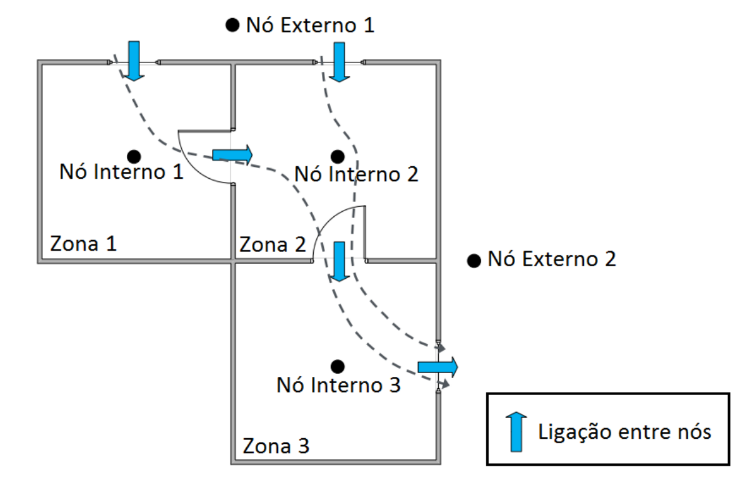
\includegraphics[width=1\linewidth]{img/nos_AFN.png}
	\label{fig:nos_AFN}
	\begin{flushleft}
		Fonte: adaptado de \citeonline{EnergyPlus2018}.
	\end{flushleft}
\end{figure}

A velocidade na qual se considera que o vento atinge a edificação modelada é obtida a partir do arquivo climático utilizado na simulação computacional. A partir das medições de velocidade do vento na estação meteorológica, extrapola-se os valores para outras altitudes e perfis de terreno. Essa consideração em relação à velocidade do vento é baseada no \textit{Handbook of Fundamentals} da \citeonline{ASHRAE2005}.
Os coeficientes do perfil de velocidade do vento são variáveis que dependem das características de rugosidade do terreno no entorno. Os valores típicos são apresentados na Tabela \ref{tab:ventoterreno}.

\begin{table}[h]
	%		\vspace{-10pt}
	\caption{Coeficientes do perfil de velocidade do vento.}
	\label{tab:ventoterreno}
	\centering
	\resizebox{\textwidth}{!}{
		\begin{tabular}{|c |c |c |c | } % \textwidth}{@{\extracolsep{\fill}} \hspace{-.33\columnwidth}
			\hline	
			\textbf{Categoria} & \textbf{Descrição do terreno} & \textbf{Expoente,} & \textbf{Espessura da camada} \\
			\textbf{do terreno} & {} & \textbf{$\alpha$} & \textbf{limite, $\delta$ (m)} \\
			\hline
			{} & Grandes centros urbanos nos quais & {} & \\
			1 & pelo menos 50\% das edificações são & 0,33 & 460 \\
			{} & maiores que 21 m. & {} & \\
			\hline
			{} & Terreno urbano, subúrbio, áreas com & {} & \\
			2 & árvores, áreas com espaçamento & 0,22 & 370 \\
			{} & entre obstruções do tamanho ou & {} & \\
			{} & maiores do que casas unifamiliares. & {} & \\
			\hline
			{} & Terreno aberto com poucas & {} & \\
			3 & obstruções, geralmente menores do & 0,14 & 270  \\
			{} & que 10 m de altura. & {} & \\
			\hline
			{} & Área desobstruída plana exposta ao & {} & \\
			4 & vento. Entorno de corpos d’água de & 0,10 & 210  \\
			{} & mais de 1,6 km. & {} & \\
			\hline
			
		\end{tabular}
	}
	\begin{flushleft}
		Fonte: adaptado de \citeonline{ASHRAE2005} (tradução do autor).
	\end{flushleft}
	%		\vspace{-12pt}
\end{table}

Os valores padrão para $\alpha_{met}$ e $\delta_{met}$, a partir dos quais se estima a velocidade do vento, são 0,14 e 270 m, respectivamente. Isso se deve ao fato de que estações meteorológicas são tipicamente estabelecidas em terrenos de categoria 3. A altura padrão é 10 m. 

Ao definir a velocidade do vento, o programa EnergyPlus calcula a pressão do vento sobre as edificações, determinada também pelo princípio da equação de Bernoulli \cite{Walton1989}.

A maior dificuldade no desenvolvimento do AFN é a necessidade de estimar as características do fluxo nas aberturas e o coeficiente de pressão do vento na edificação \cite{Arendt2017}. Os coeficientes de pressão do vento (Cp) descrevem como o vento interfere na distribuição externa de pressões em volta da edificação. 
Os Cp dependem principalmente da geometria da edificação, dos detalhes da fachada, do entorno da edificação, da velocidade e direção do vento, e da intensidade da turbulência. Na prática, 	destaca-se a dificuldade em determinar precisamente a relação entre o Cp e todos esses fatores. As abordagens mais realistas são os experimentos em escala real in-situ. No entanto, esses experimentos possuem custo elevado e normalmente possuem grandes incertezas. Os dados dos Cp podem ser estimados das seguintes fontes: testes de túnel de vento; simulações com CFD; modelos analíticos; e bases de dados.
Bases de dados de Cp são compilações de uma ou mais fontes, onde os dados são classificados de acordo com alguns parâmetros, como a forma da edificação e a orientação de incidência do vento. 

A dificuldade em se considerar toda a complexidade de variação do Cp faz com que os programas de simulação termoenergética de edificações com AFN, geralmente, incorporem métodos simplificados \cite{Costola2009}. Os experimentos de túnel de vento são as fontes primárias mais comuns. A qualidade dos resultados de túneis de vento são diretamente afetados pela calibração do túnel de vento, a garantia de qualidade dos procedimentos, e o conhecimento do pessoal para a preparação e execução dos testes.

Os túneis de vento permitem um bom grau de controle sobre os experimentos, assim como a repetitividade e reprodutibilidade dos testes conduzidos \cite{Omrani2017}. No entanto, a escala pode afetar o fluxo de ar e as transferências de calor se os parâmetros adimensionais corretos não são mantidos entre os modelos de diferentes tamanhos. Isso faz com que o ideal seja usar modelos em escala real.

Em casos em que não é possível obter os valores de Cp por fontes primárias, \citeonline{Costola2009} apontam as bases de dados como as fontes secundárias mais comuns. A base de dados de pressão de vento da Universidade Politécnica de Tóquio (TPU) oferece dados experimentais obtidos a partir de experimentos em túnel de vento \cite{TPU2018}. A base de dados possui os resultados de testes conduzidos utilizando-se modelos de acrílico em um túnel de vento de seção de 2,2 m de largura por 1,8 m de altura. A camada limite atmosférica foi simulada por elementos geradores de turbulência e outros elementos de rugosidade. Diferentes perfis de vento foram usados para construir a base de dados. Na maioria dos experimentos a velocidade média e os perfis de intensidade de turbulência estavam de acordo com as de terreno suburbano. A intensidade de turbulência à altura de 10 cm foi cerca de 0,25, e a velocidade de vento teste a essa altura foi 7,4 m/s. O número mínimo de Reynolds foi 25340, que é acima do limite 11000 para o fluxo independente.

Diversos fatores que afetam o valor do Cp são comumente simplificados, como apontado por \citeonline{Costola2010} na Tabela \ref{tab:CpSimp}.

\begin{table}[h]
	%		\vspace{-10pt}
	\caption{Fatores que afetam o Cp e simplificações comuns.}
	\label{tab:CpSimp}
	\centering
	\resizebox{\textwidth}{!}{
		\begin{tabular}{|c |c |} % \textwidth}{@{\extracolsep{\fill}} \hspace{-.33\columnwidth}
			\hline	
			\textbf{Fatores que afetam o Cp} & \textbf{Simplificações comuns} \\
			\hline
			Ponto de interesse na superfície da & Dado médio para a superfície \\
			fachada da edificação (Cp local) & (Cp médio)\\
			\hline
			Perfil do vento & Adoção de coeficientes que determinam \\
			{} & o perfil de vento de acordo com o local \\
			\hline
			Elementos de obstrução da edificação & Obstruções com formas genéricas  \\
			\hline
			Geometria da edificação e detalhes & Dados genéricos usados para \\
			da fachada & qualquer forma, e sem detalhes na \\
			{} & fachada considerados \\
			\hline
			Direção do vento & Resolução angular baixa \\
			\hline
			
		\end{tabular}
	}
	\begin{flushleft}
		Fonte: adaptado de \citeonline{Costola2010} (traduzido pelo autor).
	\end{flushleft}
	%		\vspace{-12pt}
\end{table}

De acordo com \citeonline{Costola2010}, os Cp médios se definem de acordo com Equação \ref{eq:CalcCp} e Equação \ref{eq:Pvel}.

%	\vspace{-8pt}
\begin{equation}\label{eq:CalcCp}
C_p = \frac{P_x - P_0}{P_d}
\end{equation}
%	\vspace{-5pt}
%	\vspace{-8pt}
\begin{equation}\label{eq:Pvel}
P_d = \frac{\rho V^{2}_{ref}}{2}
\end{equation}
%	\vspace{-5pt}

Onde:

$P_x$ é a pressão estática em um dado ponto da fachada do edifício ($Pa$);

$P_0$ é a pressão estática de referência ($Pa$);

$P_d$ é a pressão dinâmica ($Pa$);

$\rho$ é a densidade do ar ($kg/m^3$);

$V_{ref}$ é a velocidade do vento de referência ($m/s$).
\\

Nas simulações termoenergéticas de edificações, há muita incerteza relacionada ao Cp. Isso deve-se à influência do Cp em muitos dos indicadores de desempenho, como consumo de energia ou conforto térmico, que são frequentemente sensíveis à taxa de fluxo de ar \cite{Costola2009}. 
As bases de dados de Cp são amplamente disponíveis, particularmente para o cálculo de carga de vento em estruturas. Esses valores de Cp para edificações sem obstruções, com geometria simples, podem ser utilizados quando experimentos em túneis de vento não são disponíveis. Uma abordagem similar é usada para bases de dados de ventilação e infiltração na literatura. Nenhuma das bases de dados e modelos analíticos lidam com os efeitos da topografia local, detalhes da fachada, ou informam a incerteza dos dados disponibilizados. Os efeitos das edificações do entorno são considerados com muitas limitações e simplificações.

O estudo de \citeonline{Costola2010} quantifica a incerteza na taxa de fluxo de ar devido ao uso do Cp médio da fachada, considerando 15 formas de edifícios e diferentes configurações de aberturas. O foco se deu em ventilação e infiltração movidas por vento, e a força de empuxo não foi considerada. Este estudo apresentou a estimativa de incerteza para edificações com duas aberturas idênticas, e uma zona interna, baseando-se em uma grande faixa de formas e ângulos de incidência do vento. A incerteza na taxa de fluxo de ar calculada usando-se os coeficientes médios da superfície para edificações isoladas com duas aberturas varia entre 0,23 e 5,05 vezes o fluxo se comparada ao uso do Cp local, para um intervalo de confiança de 95\%. As grandes incertezas relativas devem-se às pequenas taxas de fluxo de ar. Quando se considera apenas as superfícies com maiores diferenças de pressão relativa, a incerteza diminui para  valores entre 0,52 e 1,42 vezes. Conclui-se que a magnitude da incerteza é alta, mas o julgamento em relação à aplicabilidade desses dados depende do problema em análise e do indicador de desempenho escolhido.

O trabalho de \citeonline{Arendt2017} estuda a influência dos dados de Cp de diferentes fontes na precisão de um modelo AFN. Uma edificação real com um sistema de ventilação movido por vento e força de empuxo foi adotado para um estudo de caso. Oito casos com diferentes dados de Cp foram estudados. Os resultados de temperatura do ar e fluxo do ar interno foram então comparados com as medições na escala real. Uma edificação residencial de dois pavimentos, localizada em Skarszewy, no norte da Polônia, foi escolhida para o estudo de caso. A edificação possui janelas e chaminés de ventilação. A densidade de construção na área de entorno da edificação não foi especificada no estudo. As simulações foram efetuadas para um período de tempo de 7 dias no fim da primavera. 
A modelagem da edificação foi realizada através do programa EnergyPlus 8.1 \cite{EnergyPlus2015}. Os valores de Cp foram obtidos de duas fontes: CPCALC+, que é um modelo analítico; e AIVC, que oferece uma base de dados. A partir dos dados do AIVC, considerou-se duas possibilidades: área plana aberta; e área rural com barreiras de vento espalhadas. A partir do CPCALC+ considerou-se as seguintes densidades de construção: 1\%, 10\% e 20\%. Para cada densidade de construção utilizada,considerou-se mais um caso onde o Cp para o ângulo de incidência de 180$^{\circ}$ teve seu valor alterado em -0,1. Essa foi uma variação arbitrária para verificar a influência nos resultados, uma vez que 180$^{\circ}$ era a direção de incidênciacpredominante do vento no local. Em todos os casos considerou-se o coeficiente de descarga (Cd) das aberturas igual a 0,6. 
Os casos mais precisos foram: o que considerou os valores da AIVC para terrenos com barreiras esparsas; e o que considerou os valores do CPCALC+ para 1\% de densidade, e variação de -0,1 no Cp para o ângulo de incidência de 180$^{\circ}$. O caso mais próximo do real obteve uma diferença relativa de 10\%, enquanto o pior caso (CPCALC+ 1\% de densidade) obteve um erro relativo de 169\%. Os erros do CPCALC+ foram maiores do que o do AIVC, mesmo considerando-se o Cp para a posição exata da abertura, enquanto o AIVC considerou a média na superfície da fachada. Nos melhores resultados, a diferença calculada para a temperatura do ar foi menor do que 0,5 $^{\circ}$C, enquanto nos piores, foi entre 1,1 $^{\circ}$C e 1,2 $^{\circ}$C. A correlação entre a precisão relativa do fluxo de ar e da temperatura do ar não foi linear. A conclusão final foi que simulações com AFN na fase inicial de projeto, quando não há dados experimentais disponíveis para a validação do modelo, possuem significantes incertezas.

\citeonline{Freire2013} avaliaram diferentes modelos de ventilação cruzada e unilateral (\textit{British Standard}, Gids e Phafe, e Larsen) e compararam com resultados de medições \textit{in-situ} e em túneis de vento. Também são avaliadas as bases utilizadas para obtenção dos Cp. 
O modelo de Larsen mostrou-se mais apropriado para a ventilação unilateral, por considerar variações em função do ângulo de incidência do vento. Os Cp do CPCALC (Cp local) obtiveram resultados mais precisos do que os das equações de \citeonline{Swami1988} (Cp médio), que é o método padrão do programa EnergyPlus \cite{EnergyPlus2018} para a obtenção do Cp. Porém, ambos obtiveram erros relativos por volta de 30\%. O fluxo de ar por grandes aberturas envolve diferentes obstáculos, que inclui desde fluxos gravitacionais estáveis, até fluxos flutuantes devido à turbulência do vento. A solução utilizada pelo programa EnergyPlus 8.9 \cite{EnergyPlus2018} para a modelagem de grandes aberturas é baseada no modelo COMIS \cite{Feustel1990}. As principais premissas para esse modelo são:

\begin{itemize}
	\item fluxo estável, fluido não-viscoso e incompressível;
	\item estratificação linear da densidade em ambos os lados da abertura;
	\item efeitos de turbulência representados por um perfil de diferença de pressão equivalente;
	\item efeitos de redução da área efetiva de abertura representados por um coeficiente.
\end{itemize}

O componente \textit{Detailed Opening} do EnergyPlus \cite{EnergyPlus2018} assume que, além da diferença de pressão entre os nós ligados pela abertura, há diferenças de pressão em função da altura da abertura, relacionadas à densidade do ar e à velocidade do vento. Por isso, é possível haver dois planos neutros de pressão ao longo da abertura, permitindo que o fluxo de ar se divida em três partes. 
Na Figura \ref{fig:DetailedOpening}, $P_{01}$ e $P_{02}$ representam as pressões nos nós, $\rho_{1}$ e $\rho_{2}$ representam a diferença de densidade do ar em função da altura, e $P_z$ representa a diferença de pressão em função da altura, causada pela turbulência do vento.


\begin{figure}[h]
	\centering
	\caption{Fenômenos considerado pelo EnergyPlus ao modelar fluxo de ar através de grandes aberturas.}
	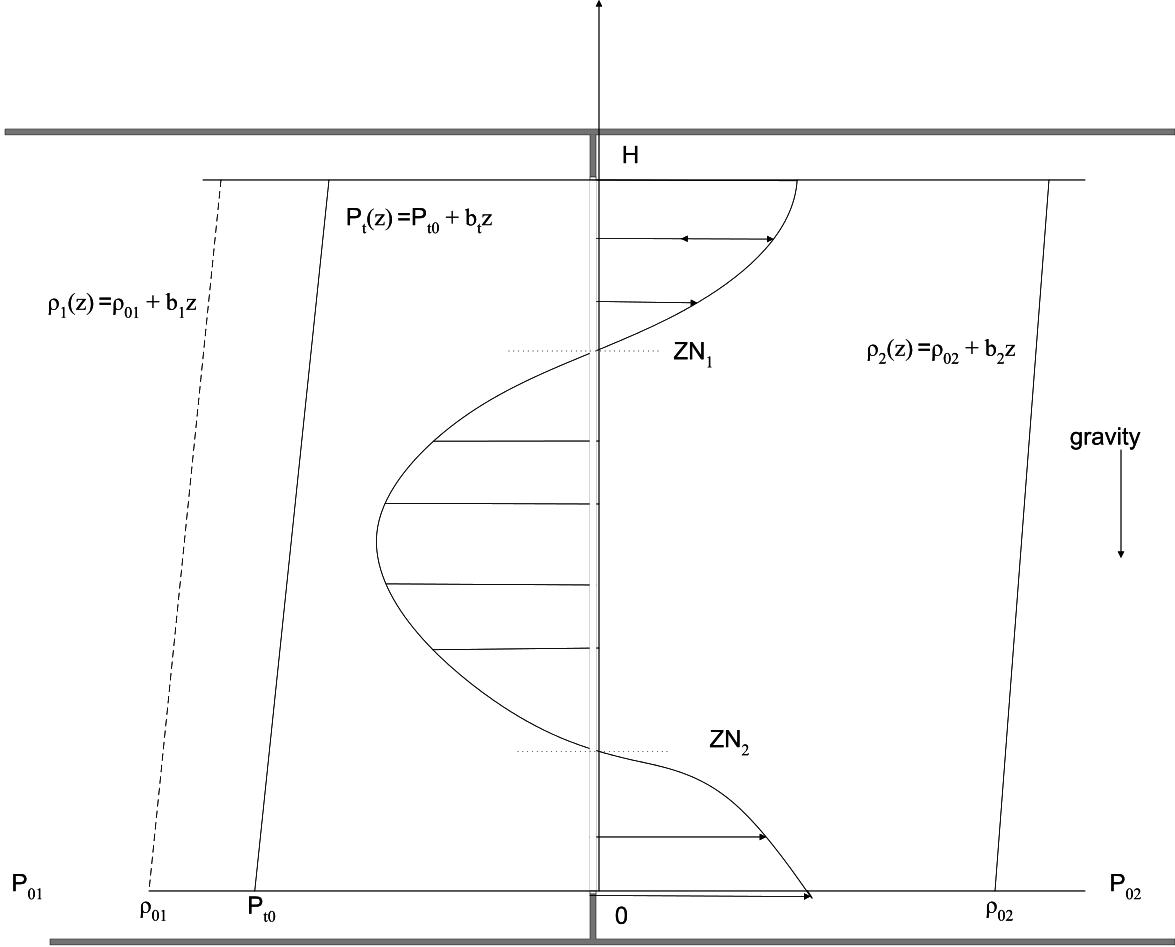
\includegraphics[width=1\linewidth]{img/detailed_opening.png}
	\label{fig:DetailedOpening}
	\begin{flushleft}
		Fonte: \citeonline{EnergyPlus2018}.
	\end{flushleft}
\end{figure}

O coeficiente de descarga (Cd) é utilizado para representar a característica do fluxo na abertura quando a abertura é grande. Para frestas, utiliza-se o coeficiente de fluxo de ar por frestas \cite{Arendt2017}.
Esses coeficientes se definem como a razão entre o fluxo real em relação ao	ideal, quando a taxa de fluxo de massa de ar de referência é a vazão mássica de ar para a diferença de pressão de 1 Pa. Ambos os parâmetros dependem da geometria da abertura, velocidade do ar, orientação geográfica, edificações do entorno, morfologia urbana e a forma do edifício em questão.
O valor do Cd é o produto entre o coeficiente de velocidade e o coeficiente de contração \cite{Flourentzou1998}. Ele pode ser determinado experimentalmente quando a taxa de fluxo de ar é medida diretamente, com gás rastreador, por exemplo. O coeficiente de velocidade também pode ser determinado similarmente medindo-se as velocidades do ar.

\citeonline{Iqbal2015} apontam que o Cd representa os efeitos não ideais de fluxo, que são causados principalmente pela fricção no caminho do fluxo de ar e o efeito de contração devido a mudanças na direção do fluxo. Devido à dificuldade de se estimar esses efeitos separadamente, normalmente apenas o Cd é usado para especificar vazão de ar através de aberturas. O valor de Cd para janelas operáveis não é constante, mas varia consideravelmente de acordo com a área de abertura, o tipo de janela e a diferença de pressão entre a abertura. O uso de valores constantes de Cd podem levar a estimativas errôneas do fluxo de ar.

De acordo com o manual do COMIS \cite{Feustel1990}, os valores de Cd podem variar de 0,61, para orifícios de arestas vivas,	até 0,98 para tubos com forma de trompete. Os valores encontrados podem variar de 0,25 até 0,75 para grandes aberturas. Normalmente assume-se o valor de 0,6 para aberturas retangulares em simulações  \cite{Flourentzou1998, Heiselberg2001, Breesch2010, Iqbal2015, Krzaczek2015, Arendt2017}.

O objetivo de \citeonline{Flourentzou1998} foi identificar os valores de coeficientes de resistência de fluxo para uma edificação de escritórios de três pavimentos naturalmente ventilada na Suíça. A ventilação por força do vento foi desconsiderada devido à sua instabilidade, o que fez com que os experimentos fossem conduzidos em noites sem vento. O estudo considerou apenas ventilação por força de empuxo, de fluxo levemente turbulento, buscando validar algoritmos simples de ventilação e dar uma base experimental para diretrizes de projeto para técnicas de resfriamento noturno. Nos experimentos, mediu-se a velocidade do ar e linha de pressão neutra, observando-se os coeficientes de contração e de velocidade usados no modelo de Bernoulli. As medições foram efetuadas levando-se em conta a ventilação unilateral e cruzada. As escadas funcionaram como uma chaminé de exaustão nas trocas de ar por empuxo. Os valores de Cd encontrados estão de acordo com o valor geralmente aceito de 0,6 ${\pm}$ 0,1.

\citeonline{Heiselberg2001} descreveram e sumarizaram os resultados de uma série de medições em laboratório, desenvolvidas para determinar as características do fluxo de ar em janelas abertas, e da distribuição de ar na sala, além de fornecer dados para projetos. O trabalho focou na estimativa dos Cd, nas condições de fluxo de ar no ambiente e no desenvolvimento de um modelo semi-empírico de fluxo para estimar parâmetros de conforto em zonas ocupadas. As medições foram aplicadas a dois tipos de janelas, e em função do ângulo de abertura e diferenças de pressão e temperatura através da abertura. Os resultados mostram que o Cd não pode ser considerado constante, pois varia consideravelmente em função da área de abertura, do tipo de janela e das diferenças de temperaturas. Isso pode levar a erros relacionados à capacidade de fluxo. O valor normalmente adotado de 0,6 é obtido apenas para áreas de abertura grandes. Áreas de abertura menores possuem valores maiores.

O estudo de \citeonline{Iqbal2015} avalia o efeito do ângulo de abertura na taxa de fluxo ar em janelas pivotantes em telhados. Os valores de Cd são obtidos para os diferentes ângulos, com e sem vento, para fluxos de entrada e saída. Utilizou-se medições em túnel de vento para o estudo, com o modelo de uma residência em escala 1:20. Os resultados são apresentados para fluxo unidirecional. Na ausência de vento, o Cd diminui com o aumento do ângulo de abertura. O Cd mostrou-se variar em função do número de Reynolds. Para fluxo turbulento totalmente desenvolvido, o Cd também diminui com o aumento no ângulo de abertura. Para fluxos de ar movidos por vento, o Cd da janela depende da turbulência na taxa de fluxo de ar que passa pela abertura. Concluiu-se que o valor de Cd varia em função da fração de velocidade (velocidade média do ar em relação à velocidade do vento de referência). Os valores de Cd para fluxos de entrada e saída foram diferentes. Quando a velocidade do ar é superior à velocidade do vento de referência, o Cd é independente da fração de velocidade e da direção do fluxo, e os valores de Cd são idênticos aos valores para velocidade do vento igual a zero. Para ângulos de abertura pequenos o Cd era próximo a 1, enquanto o valor mínimo de Cd foi igual a 0,6 para abertura máxima, valor geralmente utilizado nos modelos de AFN para grandes aberturas. Concluiu-se que janelas pivotantes podem auxiliar na obtenção de valores maiores para o Cd, que varia em relação ao ângulo de abertura.

O fluxo de ar por aberturas horizontais no programa EnergyPlus 8.9 \cite{EnergyPlus2018} é baseado no trabalho de \citeonline{Cooper1989}. Considera-se fluxo de ar por diferença de pressão entre as zonas, por diferença de densidade (causada pelas diferenças de temperatura), ou ambos os fenômenos simultaneamente. A troca de ar total entre as zonas é a soma do fluxo gerado pela diferença de pressão, mais o fluxo da força de empuxo. Porém, o fluxo de ar que desce pela força de empuxo é igual ao fluxo de ar que sobe, cancelando a parcela da força de empuxo no somatório da massa de ar que entra e sai da zona. Para a modelagem de uma escada, há a possibilidade de se considerar um plano inclinado na abertura horizontal. Essa consideração é realizada pela substituição da área de abertura por uma área de abertura efetiva.

A VN é um fenômeno complexo, dependente de diversos fatores. O uso de modelos AFN tem algumas limitações, assim como os coeficientes adotados para a aplicação dos modelos. Apesar das condições de contorno e simplificações adotadas, o AFN apresenta-se como uma solução mais compatível com programas de simulação termoenergética de edificações como o EnergyPlus, devido ao relativo baixo custo computacional e à integração já	existente aos demais algoritmos do programa.

\section{Conforto Térmico}

Dentro de uma edificação, diversos fatores podem influenciar no conforto dos ocupantes, como características acústicas, visuais ou térmicas. Devido ao foco deste trabalho, serão discutidas questões relacionadas ao conforto térmico.
A busca por conforto térmico tem influência significativa na construção de edificações e na escolha dos materiais construtivos. Esse conforto depende de fatores físicos, fisiológicos e psicológicos. De acordo com a \citeonline{ASHRAEStandard552017}, conforto térmico é o estado da mente que expressa satisfação da pessoa com o ambiente térmico que a circunda, e é estimado através de avaliação subjetiva. No estudo do conforto térmico há duas abordagens principais: o modelo estático e o modelo adaptativo. % \textit{Standard 55}
O modelo estático foi desenvolvido por \citeonline{Fanger1970a}, a partir de estudos realizados em câmaras climatizadas. As câmaras climatizadas tinham temperatura, umidade relativa e velocidade do ar controladas, e os objetos de estudo exerciam atividades e utilizavam vestimentas específicas. Neste estudo, as variáveis mais importantes que influenciam no conforto térmico são: nível de atividade; resistência térmica das roupas; temperatura do ar; temperatura radiante média; velocidade do ar; umidade relativa no ambiente.

Para determinar o nível de conforto térmico no ambiente construído, \citeonline{Fanger1970a} desenvolveu a partir dessas variáveis o “Voto Médio Predito” (PMV), uma escala para otimizar as condições de conforto térmico em um ambiente construído. A escala do PMV prediz se os ocupantes do ambiente estarão sentindo frio, calor ou neutros. Para que haja conforto térmico, é necessário que haja neutralidade térmica. A neutralidade térmica é a condição na qual a pessoa prefere que o ambiente à sua volta não esteja nem mais frio, nem mais quente.
A abordagem no modelo adaptativo é diferente da proposta no modelo estático. De \citeonline{Dear1997} afirmam que uma premissa importante do modelo adaptativo é que o ocupante da edificação não é simplesmente um receptor passivo de um dado ambiente térmico, como no caso das câmaras climáticas, mas em vez disso é um agente ativo, que interage em diversos níveis do sistema “pessoa-ambiente” via ciclos retroalimentados. As expectativas térmicas resultam da confluência de experiências correntes e passadas e práticas técnicas e culturais. Sendo assim, leva-se em conta diferenças não apenas quantitativas, mas também qualitativas entre o conforto térmico em edificações condicionadas artificialmente e naturalmente ventiladas. Baseando-se em um estudo de um banco de dados de 21 mil medições realizadas em edificações comerciais, \citeonline{Dear1997} concluíram que, em edificações ventiladas naturalmente, a tolerância dos usuários em relação à variação de temperatura é maior, e o conforto depende diretamente das temperaturas médias externas.

A relação estabelecida, define os limites inferior e superior de temperatura operativa do ambiente, a partir da temperatura externa média, e estão de acordo com as Equação \ref{eq:limInf} e Equação \ref{eq:limSup} \cite{ASHRAEStandard552017}.

%	\vspace{-8pt}
\begin{equation}\label{eq:limInf}
T_{inf} = 14,3 + 0,31 T_m
\end{equation}
%	\vspace{-5pt}
%	\vspace{-8pt}
\begin{equation}\label{eq:limSup}
T_{sup} = 21,3 + 0,31 T_m
\end{equation}
%	\vspace{-5pt}`

Onde:

$T_{inf}$ é o limite inferior da temperatura operativa para que haja conforto térmico ($^{\circ}$C);

$T_{sup}$ é o limite superior da temperatura operativa para que haja conforto térmico ($^{\circ}$C);

$T_m$ é a temperatura média do ar externo ($^{\circ}$C).
\\

A temperatura média do ar externo representa o ambiente climático externo com o qual os ocupantes da edificação estão fisiologicamente,
comportamentalmente e psicologicamente adaptados. Essa variável de entrada é baseada na média aritmética das temperaturas médias externas diárias em um período de dias, e pode ser considerada como a temperatura média mensal.

O movimento do ar influencia no conforto térmico, causando desconforto por frio em algumas situações, mas também aliviando o desconforto por calor.
Isso ocorre devido ao aumento da convecção sobre as superfícies, o que causa maior evaporação, fenômeno endotérmico. Devido a essa influência no conforto térmico, a \citeonline{ASHRAEStandard552017} permite considerar a velocidade do ar como um fator determinante na busca por um ambiente termicamente confortável. Essa consideração é baseada nos valores do  \textit{Standard Effective Temperature} (SET), que relaciona a velocidade do ar e a temperatura operativa do ambiente para ambientes climatizados.

\citeonline{DeVecchi2015} aplicaram o método adaptativo da \citeonline{ASHRAEStandard552013} para o contexto climático brasileiro, caracterizado como quente e úmido. Os resultados indicam que é possível encontrar níveis aceitabilidade térmica significativos abaixo dos limites inferiores do método adaptativo. Essa tolerância a temperaturas mais baixas deve-se ao aumento de vestimentas por parte dos ocupantes, antes de se recorrer ao aquecimento artificial. Os autores sugerem que a fixação do limite inferior de temperatura operativa em no máximo 19,5 $^{\circ}$C, para umidade relativa de 80\%, representaria mais adequadamente o comportamento dos usuários no contexto climático brasileiro.

\section{Ventilação natural em edifícios de escritórios}

Nesta parte da revisão, buscou-se identificar estudos sobre o uso da VN em edificações de escritórios. Foram identificadas as características dos edifícios relacionadas à geometria, envoltória, padrões de uso, ganhos internos, configuração das aberturas da fachada, entre outros.

Ao longo da maior parte da história, as edificações eram projetadas de forma que o potencial da VN fosse explorado ao máximo. Com a invenção do ar condicionado, a partir da segunda metade do século 20, houve um crescimento do uso de ventilação mecânica e condicionamento de ar no mundo e, com isso, a arquitetura das edificações comerciais começou a sofrer mudanças \cite{CarrilhodaGraca2016}. Associado a essas mudanças do desenho vernacular tradicional, o desenvolvimento urbano resultou em problemas particulares relacionados à demanda de resfriamento nos meses mais quentes. Os grandes centros urbanos são considerados como uma ilha de poluição. Em muitas cidades, o ambiente externo é contaminado com ruído sonoro, partículas finas, calor e gases tóxicos. A dificuldade na aplicação da VN em edifícios comerciais atualmente se deve ainda a aspectos como a necessidade da concepção do conceito desde as fases iniciais de projeto, ou até mesmo a questões estéticas.

A intensidade de ocupação em edifícios de escritórios varia de acordo com as atividades exercidas. Alguns escritórios são continuamente ocupados por computadores e equipamentos ligados constantemente, enquanto outros são pouco ocupados e têm pouco uso de computadores e iluminação \cite{Elharidi2018}.

\citeonline{Neves2019} desenvolveram um banco de dados com informações levantadas em edifícios de escritórios que operam com ventilação híbrida (VN e condicionamento artificial de ar). Para isso, 153 edifícios construídos após o ano de 1995 na cidade de São Paulo foram selecionados. Dentre os edifícios selecionados, foi realizado um levantamento de campo em 50 edifícios, obtendo-se informações relacionadas às dimensões das salas de escritórios, ao tipo de esquadria utilizado e à presença de elementos de sombreamento. As informações disponíveis em todos os edifícios do banco de dados incluem: áreas, dimensões, formato e número de pavimentos das edificações; absortância das paredes externas e coberturas; e percentual de abertura na fachada (PAF). Os autores observaram as correlações entre as características encontradas nestes edifícios. As estratégias de VN adotadas não parecem ser algo que procura-se otimizar nos projetos dos edifícios analisados. Tampouco há indicação de uma mudança nesse cenário em edificações de anos mais recentes. O que se nota é o aumento de elementos de sombreamento na fachada em razão do uso de equipamentos condicionadores de ar do tipo \textit{split}. Os autores concluem que o levantamento realizado permite a identificação das características mais recorrentes nos edifícios analisados, e os intervalos de variação nos parâmetros observados.
Isso possibilita que trabalhos relacionados ao desempenho térmico de edificações sejam desenvolvidos considerando-se características de edificações reais.

\citeonline{Belleri2014} compararam predições de desempenho de VN em estágio inicial de projeto pelo programa EnergyPlus com medições de campo. O escritório estudado localiza-se no segundo andar de um edifício de dois andares na Califórnia, Estados Unidos, e tem seu espaço dividido em dois planos abertos de 130 m2, conectados por duas grandes aberturas. Não há ventilação forçada ou sistema de resfriamento. As quatro fachadas são providas de janelas, que podem ser operadas pelos ocupantes. Há ventiladores de teto com controle variável disponíveis. Os autores partiram da simulação de um modelo simples, e modificaram gradativamente os seguintes dados de entrada, de acordo com medições em campo: temperaturas internas; controle das janelas; dados climáticos (com intervalos de 5 minutos); fatores de abertura das janelas, coeficientes de pressão do vento (baseados em medições em túnel de vento). Enquanto a simulação inicial superestimou a média das trocas de ar em 1671\%, a simulação com todas as modificações superestimou as trocas de ar em apenas 148\%. O estudo conclui que, com dados suficientes, a utilização do programa EnergyPlus com o AFN pode oferecer  estimativas informativas relacionadas ao desempenho da VN. No entanto, para melhores estimativas é necessário obter dados relacionados ao vento e ao comportamento dos ocupantes, o que pode ser dificultoso na fase de projeto.

O trabalho realizado por \citeonline{Elharidi2018} buscou identificar o desempenho energético e a qualidade do ar interno de edifícios de escritórios no Egito, propondo medidas para minimizar o uso de energia. Os dados foram levantados a partir de questionários realizados em 59 escritórios, sendo complementado por dados da literatura. Os dados registrados incluem: área interna, atividade exercida no escritório, tipo de serviço prestado na edificação, tipo de edificação, e contas de energia elétrica. Dentre as atividades nos escritórios, inclui-se contadores, agências de viagem, vendas, administração da saúde, seguros, consultores, administração de bancos, recursos humanos, e governo. As edificações de escritórios foram classificadas em quatro tipos: VN sem resfriamento; VN com resfriamento local; ventilação mecânica com resfriamento local; ventilação mecânica e resfriamento central. A maioria das edificações estudadas possui apenas ventilação natural, ou VN com resfriamento local. A estratégia adotada para resfriamento e ventilação dos edifícios foi identificada como o fator mais impactante no consumo de energia. A eficiência dos equipamentos, iluminação e sistemas de resfriamento, relacionada ao comportamento dos ocupantes, pode reduzir significativamente o consumo elétrico da edificação. 
Os edifícios com apenas VN têm os menores consumos de energia, sendo que há a possibilidade de desconforto térmico em certas épocas do ano sob essas condições. Os edifícios com VN e resfriamento local têm maior consumo de energia nos meses de verão, mas demandam menos da metade do consumo de energia dos edifícios com resfriamento central.

O estudo de \citeonline{Roetzel2014} investigou o impacto do projeto da edificação e da ocupação no conforto térmico e desempenho energético em escritórios, para identificar padrões que ajudem nas considerações relacionadas aos estágios iniciais de projeto. O estudo baseia-se no cenário A2 do \textit{International Panel on Climate Change} (IPCC), para o ano de 2030.
Uma sala de escritório celular foi modelada e simulada para três climas através do programa EnergyPlus. Os locais considerados são: Hamburgo, Alemanha; Atenas, Grécia; e Alice Springs, Austrália. Dentre as variações no projeto, considerou-se três tipos de construções: de luxo; de baixo custo inicial; e sustentável. As considerações relacionadas ao comportamento dos ocupantes foram duas: de pior cenário; e de cenário ideal. Para avaliar o conforto térmico e o desempenho energético, as simulações foram realizadas para duas condições: sem consideração de resfriamento e aquecimento para análise de conforto; e incluindo-se \textit{setpoints} para aquecimento e resfriamento.
O estudo conclui que os comportamento dos ocupantes é o que mais influencia no consumo final de energia para todos os climas investigados.
Para buscar um melhor desempenho e melhores níveis de conforto, as seguintes estratégias para o projeto da edificação são indicadas: proteção solar externa que permita iluminação natural; PAF maiores que 70\% e janelas localizadas acima do plano de trabalho; massa térmica aplicada ao piso, paredes e cobertura. Em relação ao comportamento dos ocupantes, as estratégias sugeridas são: operar ativamente as janelas durante o dia e também para a ventilação noturna; operar venezianas para aproveitar a iluminação natural, prevenindo-se de ofuscamento e calor; operar iluminação artificial dependendo da luz natural; e utilizar equipamentos de escritório com baixa potência de consumo.

\citeonline{Pesic2018} descrevem a aplicabilidade geoclimática da VN na região da Catalunha, na costa do Mediterrâneo. O objetivo é providenciar diretrizes e parâmetros básicos de eficiência energética para arquitetos, engenheiros e políticos, para que possam visualizar o potencial da VN. Três cidades foram analisadas: Barcelona; Terrassa; e Tarragona. O modelo de escritório representa um edifício de três pavimentos \textit{open-plan}. A ventilação cruzada é modelada considerando-se a passagem de ar por janelas operáveis, com movimento gerado primariamente por força do vento. A orientação da edificação foi definida perpendicularmente à principal direção do vento nos meses em que a VN é mais favorável. O PAF é definido como 40\% e a infiltração na envoltória é considerada constante, com 0,25 trocas de ar por hora. As temperaturas limite de aceitabilidade do ar externo para VN é entre 10 $^{\circ}$C e 33,5 $^{\circ}$C. O horário de ocupação é das 8h00 às 18h00, e a ventilação noturna é das 21h00 às 7h00. Considerou-se a possibilidade de uso de condicionamento de ar para aquecimento e resfriamento, ou ventilação mecânica (HVAC) entre as 6h00 e 18h00. A ocupação foi considerada apenas nos dias de semana. A construção e isolamento da edificação foram definidos de acordo com os padrões da Passivhaus, padrão de construção baseado no uso de isolamento térmico da edificação. A VN foi considerada entre os dias 1º de abril e 31 de outubro (meses quentes). Seis modos de resfriamento foram considerados na análise: apenas HVAC; VN ou HVAC; VN ou HVAC, e ventilação noturna; VN e HVAC simultaneamente; VN e HVAC simultaneamente, e ventilação noturna; apenas ventilação noturna. O maior potencial de redução de energia foi observado para o uso simultâneo de HVAC e VN, com ventilação noturna. Em relação ao caso com apenas HVAC, a redução relativa foi de 28,4\%, em Tarragona, a 40,9\%, em Barcelona.

O estudo de \citeonline{Yao2009} buscou um método de analisar estrategicamente o uso de VN nas etapas iniciais de projeto. Consideraram-se as condições climáticas locais, tipo de edificação, padrões de ocupação e ventilação. O trabalho é desenvolvido a partir de um modelo de escritório para cinco climas da China: muito frio; frio; verão quente e inverno frio; verão quente e inverno ameno; e ameno. Os escritórios na China se dividem em dois tipos principais: de alto padrão com sistema central de ar condicionado; e escritório tradicional com ar condicionado \textit{split}. O modelo de escritório utilizado para o estudo possui as seguintes características: sala com dimensões 3,6 m x 5,4 m x 3,0 m; orientação sul-norte; PAF de 0,35 na parede sul e 0,25 na parede norte; ocupação das 8h00 às 18h00; capacidade térmica média; elementos de sombreamento interno na fachada sul no verão; tipo de terreno urbano; ganhos internos igual a 25 W/m2. Os autores concluem que em zonas de clima ameno a VN é altamente recomendável para edifícios de escritório em ambos os turnos. A ventilação cruzada tem maior eficiência do que a ventilação unilateral.
Em zonas de verão quente e inverno ameno, o uso de VN não satisfaz as exigências para conforto térmico. Portanto, o resfriamento mecânico é recomendado. Observou-se que o uso unicamente da ventilação noturna a não é adequada para edifícios de escritórios, pois os ganhos internos gerados ao longo do dia não podem ser liberados, causando desconforto térmico. 

\citeonline{Yun2008} comentam a dificuldade de se modelar o comportamento dos ocupantes, e como esse aspecto é uma barreira na exploração do uso de técnicas passivas e mistas de eficiência energética. Um estudo de caso foi conduzido durante o verão em seis salas de escritório com VN, localizados em Cambridge, Reino Unido. Os escritórios são ocupados por uma ou duas pessoas, e têm o PAF variando entre 0,12 e 0,57. Dentre os objetivos do estudo, buscou-se examinar o potencial da VN como estratégia de conforto e resfriamento. Foram coletados dados relacionados à posição das janelas e temperaturas internas e externas, além da aplicação de questionários.
Dos casos analisados, o que obteve melhor índice de conforto foi o escritório com brise externo e com possibilidade de aplicação de ventilação noturna. O caso com maior desconforto por calor possui uma janela com PAF de 0,57 orientada para oeste, sem sombreamento externo. As análises mostram que elementos do projeto como a orientação da fachada, o tamanho da janela em relação à orientação, a possibilidade de ventilação natural pela janela, e o sombreamento externo por brise ou edificações vizinhas são fatores determinantes no desempenho térmico. Os autores apontam que áreas envidraçadas menores podem melhorar o desempenho térmico, mas podem comprometer o uso da iluminação natural. Portanto, é crucial buscar um equilíbrio entre o uso de iluminação natural e a busca por minimizar os ganhos de calor pela fachada. Os resultados sugerem que a VN como um método de resfriamento passivo nem sempre é efetiva, pois os ocupantes nem sempre operam as janelas de acordo com as condições ideais para o resfriamento por ventilação. Portanto, destaca-se a importância de se elaborar um projeto robusto para a edificação, para compensar comportamentos desfavoráveis por parte dos ocupantes.

De acordo com \citeonline{CarrilhodaGraca2016}, nos climas quentes, que é o caso do Brasil, há maior potencial de economia e maior desafio na aplicação de VN. \citeonline{Roetzel2014} afirmam que o modelo adaptativo da \citeonline{ASHRAEStandard552017} tem uma faixa maior de aplicabilidade em climas mais quentes, o que pode propiciar um maior potencial de otimização.
Esta parte da revisão bibliográfica apresentou estudos que abordam o potencial de VN como uma solução para o resfriamento passivo em edificações de escritórios. Nos diferentes casos e configurações dos sistemas de resfriamento considerados, algumas características avaliadas e soluções propostas são predominantes, como o uso de ventilação cruzada ou de sombreamento das aberturas.
No entanto, a variação de determinadas características das edificações podem resultar em desempenhos térmicos diferentes de acordo com as combinações de parâmetros, ou características climáticas 

\section{Análise de sensibilidade}

Análise de sensibilidade (AS) é uma ferramenta valiosa na simulação termoenergética de edificações. Por isso, a AS é usada amplamente para explorar as características do desempenho térmico em edificações em diversas aplicações, como projetos, calibração de modelos, \textit{retrofits}, impacto das mudanças climáticas entre outros \cite{Tian2013a}. A metodologia para a aplicação da AS tipicamente adota os seguintes passos: determinar as variações dos dados de entrada; determinar os modelos das edificações; executar as simulações dos modelos; coletar os resultados; executar a AS; apresentar os resultados da AS. Os métodos de AS podem ser divididos entre as abordagens local e global. A AS local é focada nos efeitos da incerteza de parâmetros de entrada em torno de um caso base, enquanto a AS global é mais interessada na influência dos parâmetros de entrada sobre todo o espaço de parâmetros de entrada possíveis. Por isso, a AS global é considerada mais confiável. A AS global inclui métodos de regressão, baseados em screening, em variância e metamodelos.

O primeiro passo para realizar uma AS é determinar a faixa dos dados de entrada. Quando o objetivo é determinar diferentes opções de projeto,  \citeonline{Tian2013a} sugere distribuições uniformes nos dados de entrada, pois assume-se que os diferentes valores para os dados de entrada são igualmente prováveis.

O método da variância decompõe a incerteza dos dados de saída para seus correspondentes dados de entrada  \cite{Tian2013a}. Nessa abordagem, os dois métodos mais comuns são o FAST \cite{Saltelli2004} e o \citeonline{Sobol1993}. 
Por esses métodos, é possível avaliar efeitos de primeira ordem e de ordens superiores.
Os efeitos de primeira ordem são determinados observando-se o quanto a variação de cada parâmetro isoladamente influencia na variância dos dados de saída.
Os efeitos de segunda ordem consideram as interações entre dois parâmetros na variância dos dados de saída, e a mesma lógica segue para os efeitos de ordens superiores.
Os efeitos totais, para cada parâmetro, são a soma dos efeitos de todas as ordens.
Ao somar os efeitos de primeira ordem mais os efeitos de ordens superiores, de todos os parâmetros do modelo, o valor obtido deve ser igual a 1.
Quando o objetivo é fixar parâmetros não impactantes nos resultados, os efeitos totais devem ser usados \cite{Saltelli2004}. Métodos de variância são de abordagem livre, fazendo com que sejam adequados para modelos não-lineares e com correlações entre variáveis.

\section{Metamodelos de eficiência energética e desempenho térmico em edificações}
Projetistas encontram dificuldades no uso de ferramentas de simulação de desempenho energético, que podem não ser compatíveis com suas necessidades e métodos de trabalho. Por isso, \citeonline{Picco2014a} propõem simplificar a descrição do edifício e converter um modelo detalhado em um modelo simplificado, com apenas um número limitado de entradas. Em um estudo de caso, simplificações foram assumidas quanto às envoltórias, superfícies transparentes, zonas térmicas e pavimentos de um edifício comercial. As diferenças encontradas em relação ao modelo detalhado, no pior caso, foram de 15,6\% para cargas de aquecimento e 14,6\% para cargas de resfriamento. Com diferenças menores de 4\% e 9\% para cargas de pico, respectivamente. Apesar das margens de erro, os autores observaram que simplificações no modelo podem auxiliar em estágios iniciais de projeto, quando certas características no projeto do edifício ainda não estão bem definidas.

Há modelos baseados em equações físicas, que simulam os sistemas de transferência de calor, e modelos baseados em funções estatísticas, que deduzem esses comportamentos. Modelos estatísticos funcionam apenas com entradas e saídas, sem correlacionar causa e efeito, mas têm maior agilidade. 
Os modelos escritos com equações físicas seguem os princípios da conservação de energia e são os que mais se aproximam do comportamento real, mas podem ser dificultosos de se aplicar por serem muito complexos. Para adaptar as principais funcionalidades de ambos os modelos, existem modelos híbridos, chamados metamodelos.

Modelos preditivos são funções matemáticas que, aplicadas a uma quantidade significativa de dados, conseguem identificar padrões ocultos e prever o que poderá ocorrer. Os métodos de inteligência artificial mais utilizados para predição de desempenho energético de edificações são redes neurais artificiais (RNA) e máquinas de vetores de suporte (MVS) \cite{Zhao2012}. São modelos altamente eficazes na solução de problemas não-lineares. Esses métodos podem oferecer predições altamente precisas, desde que as definições do modelo e parâmetros estabelecidos estejam definidos adequadamente. Modelos de RNA já foram usados para analisar vários tipos de consumo de energia em edificações em diversas condições, como em cargas de aquecimento e resfriamento, consumo de eletricidade, operação e otimização de componentes, e estimativa de parâmetros de uso. O uso de MVS vem crescendo em pesquisas e indústria. Em muitos casos as MVS mostram performances superiores às das RNA, mesmo com pequena quantidade de dados para treinamento.

Os resultados de simulações podem ser avaliados a partir de características específicas. Essas características podem incluir pico da demanda de energia, consumo anual de energia, conforto, custo do ciclo de vida, entre outros. No desenvolvimento de um metamodelo analítico para otimização de modelos de energia de edificações, \citeonline{Eisenhower2012} utilizaram o PMV para a avaliação dos resultados. A caracterização dos dados e técnica de regressão do modelo foram baseadas em princípios de aprendizagem automática. Aprendizagem automática é uma classificação de algoritmos que tentam identificar características dentre os dados, sem conhecimento prévio dessas características. 
Dentre diferentes possíveis abordagens (RNA, Programação Genética, Redes Bayesianas) a escolhida para o caso foi a MVS. 
A identificação dos parâmetros mais influentes no processo de otimização foi realizada através de uma análise de sensibilidade global, baseada em derivadas locais. O metamodelo gerado foi capaz de identificar a minimização do consumo de energia, mantendo ou melhorando o conforto, sem necessidade de extensivas repetições de simulações de energia.

\citeonline{Rackes2016} propõem um metamodelo para analisar edificações comerciais e escolas de poucos pavimentos, ventiladas naturalmente. Primeiramente, foi construído um banco de dados com aproximadamente 50.000 simulações. As simulações foram executadas a partir dos modelos termoenergéticos e AFN do programa EnergyPlus, e do modelo de conforto adaptativo da  \citeonline{ASHRAEStandard552013}, que determina a zona de conforto que satisfaz 80\% dos ocupantes. As características dos edifícios simulados foram variadas a partir de 55 dados de entrada relacionados à tipologia do edifício, layout interno, geometria das janelas e sombreamento, propriedades do fluxo de ar, materiais de construção, cargas internas e transferência de calor pelo solo. Os arquivos de IDF utilizados pelo EnergyPlus foram criados a partir de uma rotina escrita no programa MatLab. Foram utilizados 427 arquivos climáticos do Brasil para a representação geográfica. 
O indicador de desempenho em conforto térmico escolhido foi o \textit{Exceedance Hour Fraction} (EHF), que é a fração de horas de desconforto em relação às horas de ocupação. Na etapa seguinte, 93 parâmetros preditores foram definidos para a análise do banco de dados. A principal ferramenta para a análise de sensibilidade foi a regressão linear múltipla da variável resposta em relação aos preditores. O método de aprendizagem automática escolhido foi a MVS. Após treinar e avaliar diversos modelos, 53 parâmetros preditores foram selecionados para a versão final. Esses parâmetros podem ser obtidos a partir de 29 dados de entrada e um arquivo climático. Comparando as simulações do EnergyPlus com as predições, o metamodelo apresentou RMSE (erro médio quadrático) igual a 0,059 e AE95 (erro absoluto do 95o percentil) igual a 0,126. Quando testado com outros 2000 casos não usados no treinamento do metamodelo, o RMSE foi 0,060 e o AE95 foi 0,129, o que indica consistência nos resultados. 

\citeonline{Versage2015} desenvolveu um metamodelo para estimar a carga integrada anual de energia de refrigeração para avaliação de desempenho energético de edificações condicionadas artificialmente através do desempenho individual de suas zonas térmicas. Foi desenvolvida uma base de dados de aproximadamente 1,29 milhões de casos simulados, com parâmetros construtivos variados, para o clima de Florianópolis. Uma amostra dos dados foi adotada para a elaboração de metamodelos com as técnicas de regressão linear múltipla, regressão adaptativa multivariada por \textit{splines}, processo gaussiano, máquina de vetores de suporte, \textit{random forest} e redes neurais artificiais. Para avaliar e comparar os metamodelos, quatro índices de desempenho foram escolhidos: tempo de treinamento, coeficiente de determinação (R$^2$), RMSE e erro médio quadrático normalizado (NRMSE). O metamodelo de RNA obteve o melhor desempenho entre os testados. A rede neural artificial treinada com 1\% dos casos do banco de dados, e com 72 nós na camada interna, obteve o melhor desempenho global, e foi capaz de reproduzir resultados com erros menores que 10\% para 99,2\% do casos. O metamodelo elaborado a partir de MVS obteve o pior desempenho. Porém, o autor destaca que outras configurações e tratamentos dos dados poderiam mudar o desempenho dos metamodelos avaliados.

\chapter{Metodologia}
\label{chapter:metodologia}

\section{Definição dos parâmetros de entrada e saída}

\subsection{Parâmetros de entrada}\label{subsec:par}

A princípio, a definição dos parâmetros adotados para gerar a base de dados de simulações para o desenvolvimento do metamodelo foram obtidos a partir do banco de dados com 153 edificações de escritórios com ventilação natural (VN) disponibilizado por \citeonline{Pereira2018}.  		
Dentre as informações  disponíveis no banco de dados, obtém-se:

\begin{itemize}
	\item orientação solar do edifício;
	\item número de pavimentos;
	\item forma dos pavimentos e das salas;
	\item áreas dos pavimentos e das salas;
	\item altura do pé-direito das salas;
	\item relações entre as dimensões dos pavimentos e entre as dimensões das salas;
	\item absortância das paredes externas; % 0.2 - 0.8
	%			\item espessura das paredes externas;
	\item cor da cobertura;
	\item tipo de vidro nas janelas;
	\item tipo de esquadria;
	\item fator de abertura das janelas;
	%			\item altura das esquadrias;
	\item percentual de abertura na fachada (PAF);  % 0 - 80
	\item tipo de sombreamento;  % 0 - 80
	\item tipo de estratégia de VN (unilateral ou cruzada).
\end{itemize} 

Os valores desses parâmetros foram observados através de suas distribuições de ocorrência. Desta forma definiu-se os limites mínimos e máximos para o desenvolvimento das simulações termoenergéticas, com parâmetros variando de acordo com o que se encontra comumente em edifícios reais. Como as edificações do banco de dados localizam-se na cidade de São Paulo, esse foi o clima para qual o metamodelo foi desenvolvido.

Certas informações não estão disponibilizadas pelo banco de dados analisado, como algumas relacionadas às propriedades termofísicas dos materiais da envoltória, às densidades de potência de iluminação e equipamentos, e aos padrões e taxas de ocupação. Frente a essa limitação, os valores desses parâmetros foram definidos a partir da Proposta de Instrução Normativa do Inmetro para a Classe de Eficiência Energética de Edificações Comerciais, de Serviços e Públicas \cite{INIC}. %, através da Tabela 4.1, da Tabela A.1 do anexo A e da Tabela B.I.1 do anexo B.  % Hora início e fim: 8 - 18,  INI-C

A Tabela \ref{table:paramconst} apresenta os parâmetros que mantiveram-se com valores constantes no desenvolvimento do trabalho. Esses valores foram escolhidos a partir do que é apresentado na \citeonline{INIC} para a simulação das edificações nas condições de referência. A cobertura tem suas propriedades termofísicas baseadas na consideração de uma laje de concreto de 10cm de espessura e telha de fibrocimento, separadas por uma câmara de ar. O padrão de ocupação foi definido de acordo com o que é estabelecido para a análise de conforto térmico em edificações de escritórios pelo método simplificado, considerando-se apenas dias de semana. Valores relacionados às propriedades termofísicas do piso em contato com solo e da laje entre pavimentos não são especificados pela INI-C, portanto foi considerado, para ambos os casos, uma laje de concreto de 12cm de espessura com uma camada de piso cerâmico.

\begin{table}[h]
	\centering
	\caption{Parâmetros com valores constantes.}
	\label{table:paramconst}
	\begin{tabular}{|l |r |}
		\hline
		\textbf{Parâmetros} & \textbf{Valores} \\
		\hline
		Capacidade térmica da cobertura & 233 kJ/m$^2$K \\
		\hline
		Transmitância da cobertura & 2,06 W/m$^2$K \\
		\hline
		Capacidade térmica do piso / laje & 306 kJ/m$^2$K \\
		\hline
		Transmitância do piso / laje & 4,30 W/m$^2$K \\
		\hline
		Transmitância do vidro & 5,7 W/m$^2$K \\
		\hline 
		Densidade de potência de iluminação & 14 W/m$^2$ \\
		\hline 
		Densidade de potência de equipamentos & 97 W/pessoa \\
		\hline 
		Hora de início de ocupação & 8 horas \\
		\hline 
		Hora final de ocupação & 18 horas \\
		\hline 
	\end{tabular}
	%			\begin{flushleft}
	%				Fonte: \citeauthoronline{INIC} \cite{INIC}, adaptado pelo autor.
	%			\end{flushleft}				
\end{table}

Os parâmetros da Tabela \ref{table:paraminic} tiveram seus limites mínimos e máximos baseados nos limites apresentados na \citeonline{INIC} para a aplicação do método simplificado. Tanto edificações condicionadas artificialmente, quanto edificações naturalmente ventiladas ou híbridas têm limites semelhantes para a aplicação do método.
A única excessão é a taxa de ocupação, que é sempre considerada com o valor fixo de 0,10 pessoas/m$^2$ na \citeonline{INIC}. No entanto, sabendo-se da influência que a carga térmica proveniente dos ocupantes e equipamentos elétricos pode ter nas temperaturas internas das zonas térmicas, optou-se por variar a taxa de ocupação entre a metade e o dobro do que é definido pela Instrução Normativa. A densidade de potência dos equipamentos foi definida com um valor constante, mas varia de acordo com a taxa de ocupação, como apresentado previamente na Tabela \ref{table:paramconst}.

\begin{table}[h]
	\centering
	\caption{Limites mínimos e máximos de valores dos parâmetros variáveis não disponíveis no banco de dados.}
	\label{table:paraminic}
	\begin{tabular}{|l |r |}
		\hline
		\textbf{Parâmetro} & \textbf{Faixa de valores} \\
		\hline
		Capacidade térmica da parede & 0,22 - 450 [kJ/m$^2$K] \\
		\hline
		Transmitância da parede & 0,50 4,40 [W/m$^2$K] \\
		\hline
		Fator solar do vidro & 0,20 - 0,87 [-] \\
		\hline 
		Ângulo horizontal de sombreamento & 0 - 80 [$^{\circ}$] \\
		\hline 
		Taxa de ocupação & 0,05 - 0,20 [pessoas/m$^2$] \\
		\hline 
	\end{tabular}
	%			\begin{flushleft}
	%				Fonte: \citeauthoronline{INIC} \cite{INIC}, adaptado pelo autor.
	%			\end{flushleft}				
\end{table}

\subsection{Parâmetro de saída}

A variável de saída do metamodelo desenvolvido é a fração de horas de desconforto por calor (EHF). Neste trabalho, o indicador escolhido para o limite superior da temperatura é estabelecido pelo método de conforto adaptativo da \citeonline{ASHRAEStandard552017}, para 80\% de satisfação entre os ocupantes. O desconforto por frio não foi considerado.
A Figura \ref{fig:temp_means} apresenta as temperaturas externas da cidade de São Paulo, com suas médias mensais, e os limites superiores de temperatura pelo método de conforto adaptativo da \citeonline{ASHRAEStandard552017}, para 80\% de satisfação entre os ocupantes.

\begin{figure}[H]
%	\vspace{0pt}
	\centering
	\caption{Temperaturas externas da cidade de São Paulo, e limites superiores de aceitabilidade}
	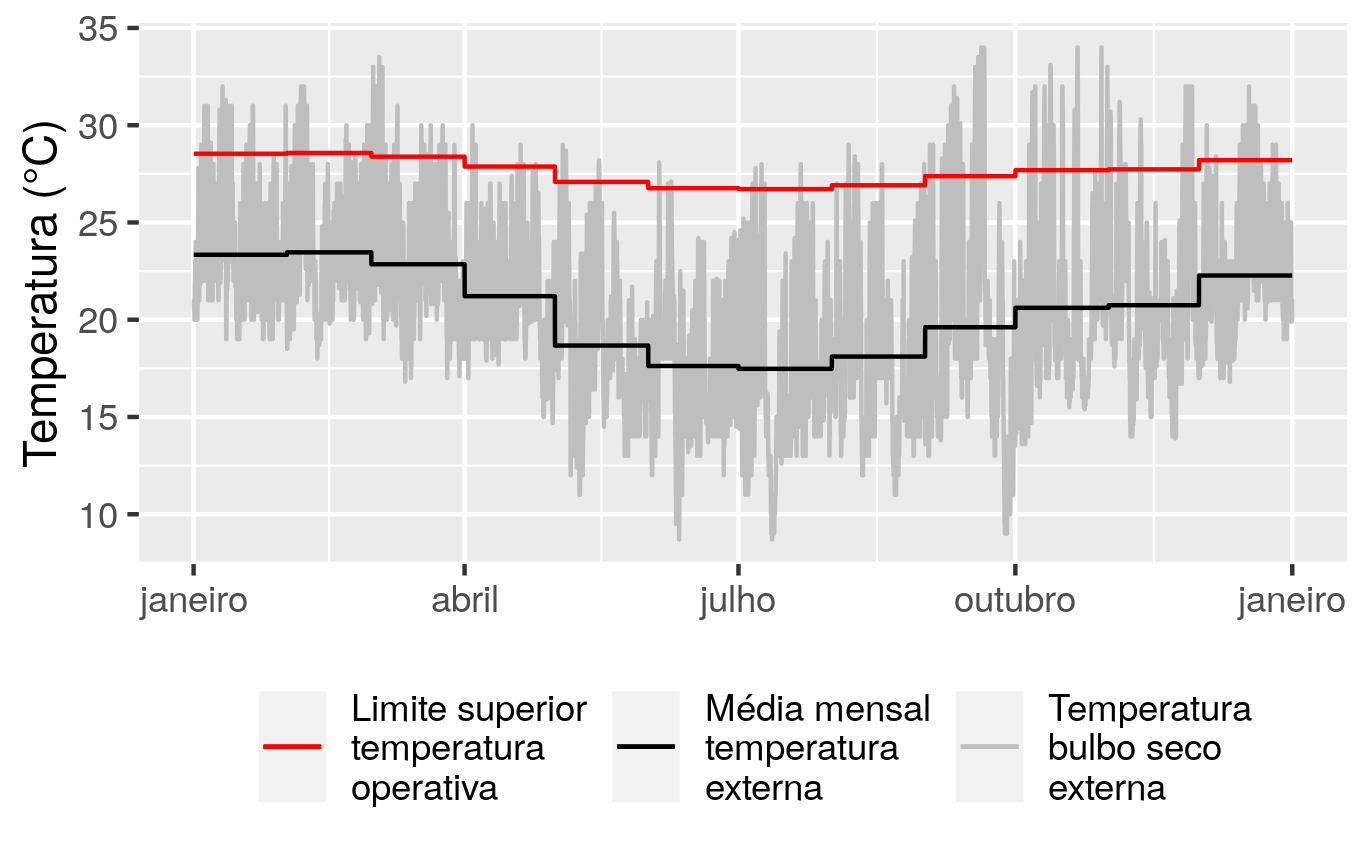
\includegraphics[width=.9\linewidth]{img/temp_means.png}
	\label{fig:temp_means}
%	\vspace{-5pt}
\end{figure}

Durante as simulações, para cada \textit{timestep} com ocupação na sala, foi calculado se a temperatura operativa da zona térmica ultrapassou o limite superior determinado pelo método adaptativo da \citeonline{ASHRAEStandard552017}. Ao fim de cada simulação, a fração de horas de desconforto foi obtida para cada zona térmica modelada, de acordo com a Equação \ref{eq:EHF}:

\begin{equation}
\label{eq:EHF}
EHF = \frac{timesteps_{sup}}{timesteps_{ocup}}
\end{equation}

Onde:

$EHF$ é igual a fração de horas de desconforto por calor na zona térmica;

$timesteps_{sup}$ é igual ao número de \textit{timesteps} em que há ocupação na zona térmica e a temperatura operativa ultrapassa o limite superior determinado pelo método adaptativo;

$timesteps_{ocup}$ é igual ao número de \textit{timesteps} em que há ocupação na zona térmica.
\\

Para avaliar o potencial do uso de ventiladores, o movimento do ar foi considerado no desenvolvimento do metamodelo.
A \citeonline{ASHRAEStandard552017} considera um aumento no limite superior da faixa de conforto térmico de acordo com a velocidade do ar.
O aumento de aceitabilidade da temperatura operativa foi considerado para os três valores de velocidade do ar apresentados na Tabela \ref{table:var}, além da possibilidade se assumir o valor de velocidade do ar igual a zero, caso o uso de ventilador não tenha sido considerado.

\begin{table}[h]
	\centering
	\caption{Aumento no limite superior da faixa de conforto em relação à velocidade do ar.}
	\label{table:var}
	\begin{tabular}{|c |c |}
		\hline
		\textbf{Velocidade média do ar} & \textbf{Temperatura} \\
		\hline
		0,6 m/s & 1,2 $^{\circ}$C \\
		\hline
		0,9 m/s & 1,8 $^{\circ}$C \\
		\hline
		1,2 m/s & 2,2 $^{\circ}$C \\
		\hline 
	\end{tabular}
	\begin{flushleft}
		Fonte:  \citeonline{ASHRAEStandard552017}.
	\end{flushleft}				
\end{table}

Como o modelo de ventilação natural do programa EnergyPlus não calcula a velocidade do ar dentro das zonas, a consideração foi aplicada após as simulações, no momento da avaliação do conforto térmico em cada \textit{timestep}. A consideração da velocidade do ar foi realizada de acordo com a Equação \ref{eq:Tsup}.

\begin{equation}
\label{eq:Tsup}
T_{sup} = T_{sup,0} + T_{v_{ar}}
\end{equation}

Onde:

$T_{sup}$ é igual à temperatura limite superior na faixa de conforto, considerando-se a velocidade do ar ($^{\circ}$C);

$T_{sup,0}$ é igual à temperatura limite superior na faixa de conforto definida pelo método adaptativo, sem considerar a velocidade do ar ($^{\circ}$C);

$T_{v_{ar}}$ é igual à margem extra de temperatura permitida pela consideração da velocidade do ar ($^{\circ}$C).
\\

\section{Simulação termoenergética}

\subsection{Simulação detalhada}

Sabendo-se que o metamodelo prediz o conforto térmico baseado no método adaptativo da \citeonline{ASHRAEStandard552017}, o principal dado de saída a se obter nas simulações foi a temperatura operativa da zona térmica, assim como a temperatura do ar externo. Portanto, todo o desenvolvimento das simulações termoenergéticas do trabalho foi voltado para que se obtivesse, com boa precisão, a temperatura operativa das zonas térmicas e, posteriormente, a sua relação com a temperatura do ar externo, chegando-se ao indicador de conforto térmico.

%		A Tabela \ref{table:parametros} apresenta os parâmetros que serão considerados no desenvolvimento dos modelos, com suas faixas de valores admitidos.	
%		
%		\begin{table}[h]
%			\centering
%			\caption{Parâmetros considerados e variação nos valores.}
%			\label{table:parametros}
%			\begin{tabular}{|l |r |}
%				\hline
%				\textbf{Parâmetro} & \textbf{Valores admitidos} \\
%				\hline
%				Área da zona & 12 - 100 [m$^2$] \\
%				\hline
%				Razão entre largura e profundidade & 0,5 - 2,0 [-] \\
%				\hline
%				Altura do pavimento & 0 - 30 [m] \\
%				\hline 
%				Azimute do eixo principal & 0 - 359 [$^{\circ}$] \\
%				\hline 
%				Pé-direito & 2,4 - 3,2 [m] \\
%				\hline 
%				Percentual de abertura da fachada & 0,1 - 0,6 [-] \\
%				\hline 
%				Fator de abertura da janela & 0,1 - 1 [-] \\
%				\hline 
%				Fator solar do vidro & 0,30 - 0,87 [-] \\
%				\hline 
%				Transmitância da parede & 0,5 - 4,7 [W/m$^2$K] \\
%				\hline 
%				Capacidade térmica da parede & 20 - 400 [kJ/m$^2$K] \\
%				\hline 
%				Absortância da parede & 0,2 - 0,9 [-] \\
%				\hline 
%				Sombreamento & 0 - 50 [$^{\circ}$] \\
%				\hline 
%				Densidade de ocupação & 0,05 - 0,50 [pessoas/m$^2$] \\
%				\hline 
%			\end{tabular}
%			\begin{flushleft}
%				Fonte: o autor.
%			\end{flushleft}				
%		\end{table}

As simulações foram realizadas através do programa de simulação computacional EnergyPlus 8.9 \cite{EnergyPlus2018} e os modelos simulados foram obtidos a partir da parametrização de uma tipologia base, que permite a variação de diferentes parâmetros.  % variados pelo método de amostragem do hipercubo latino (HCL).
A maioria desses parâmetros são numéricos e podem ser variados de forma contínua. 
Inicialmente, cada simulação representou um pavimento de uma edificação com seis salas de escritórios, onde cada sala representava uma zona térmica (Figura \ref{fig:croqui}).
O solo foi modelado pelos objetos do \textit{Ground Domain}, nos casos onde o contato com solo foi considerado. As superfícies superiores e inferiores consideradas ajacentes a outros pavimentos do edifício foram modeladas como adiabáticas.

\begin{figure}[h]
	\centering
	\caption{Croqui da tipologia base}
	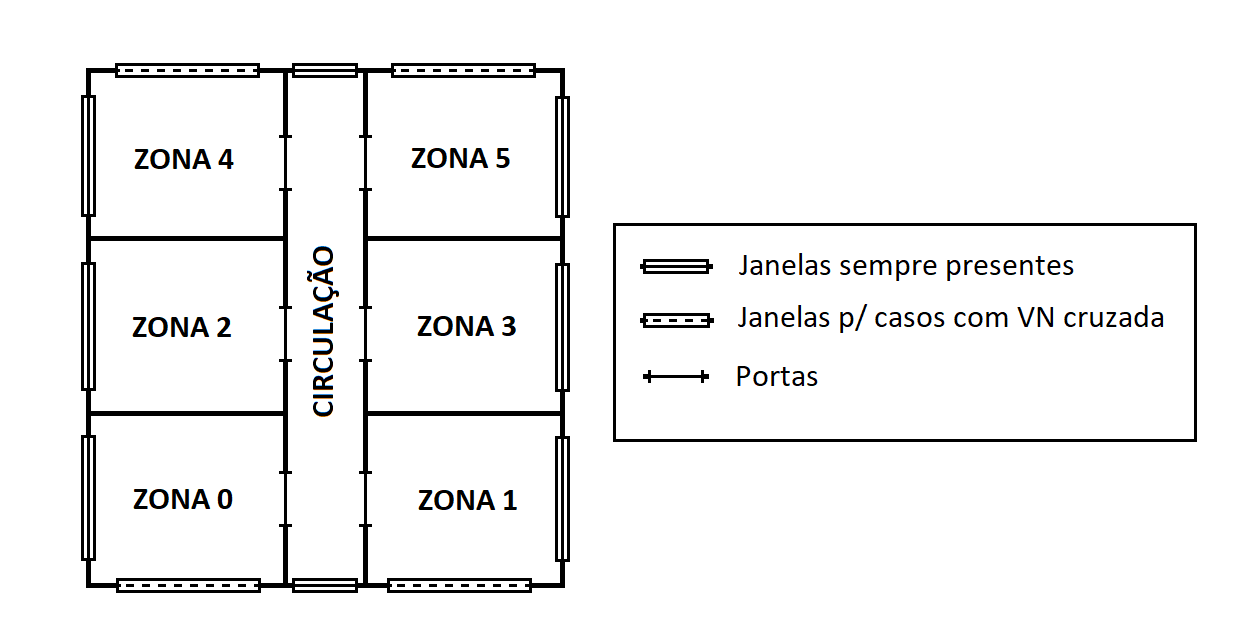
\includegraphics[width=1\linewidth]{img/croqui_07-11.png}
	\label{fig:croqui}
	%			\begin{flushleft}
	%				Fonte: o autor.
	%			\end{flushleft}
\end{figure}


A partir da tipologia base, foi possível definir diferentes proporções geométricas, levando-se em consideração a largura e profundidade da edificação, assim como o pé-direito. Também foram parametrizadas a altura do pavimento e a orientação solar da edificação.
Devido a limitações na obtenção dos coeficientes de pressão (Cp) para as faces externas da edificação, as edificações foram modeladas com pavimentos de forma retangular.

A parametrização nas propriedades termofísicas das paredes e vidros permitiu a consideração de diferentes materiais construtivos, possibilitando a descrição de uma quantidade significativa do universo de casos aplicáveis às edificações de escritórios consideradas. %Foram parametrizadas a transmitância térmica, capacidade térmica e absortância.

Para considerar o uso de ventilação natural (VN), é fundamental a modelagem das trocas de ar nos escritórios. A modelagem da VN nas simulações foi realizada com os objetos do \textit{AirflowNetwork} (AFN) do EnergyPlus \cite{EnergyPlus2018}.
Para possibilitar trocas de ar, elementos de ligação do AFN foram modelados em todas as zonas térmicas.
Todas as aberturas foram modeladas utilizando-se o objeto \textit{AirflowNetwork:MultiZone:Component:DetailedOpening}.
Cada sala foi modelada com uma porta, voltada para a circulação.
Na circulação, além das portas das salas, duas janelas foram modeladas, uma em cada extremidade. 
Salas com apenas uma fachada foram modeladas com uma janela; salas com duas fachadas foram modeladas com uma ou duas janelas. Isso possibilitou explorar casos com diferentes configurações de exposição das superfícies, considerando-se VN unilateral e cruzada.		
As dimensões das janelas das salas foram parametrizadas de acordo com o percentual de abertura da fachada (PAF), permitindo diferentes frações de abertura para representar diferentes modelos de janela encontrados nas edificações de escritórios existentes no banco de dados.
%Além da área da abertura ter influência direta nas trocas de ar das zonas, a altura também pode ter influência devido à força de empuxo causada pelas diferenças de densidade do ar. Devido a isso, a altura da janela também foi parametrizada.
%		Para o vidro das janelas considerou-se diferentes valores para o fator solar.
%		\subsection{Ventilação natural no modelo preliminar}
O controle das janelas foi estabelecido pela diferença de temperatura entre o ar externo e o ar da zona.
As trocas de ar nas portas foram modeladas apenas por frestas, por considerar-se que portas de escritórios não ficam abertas normalmente.  % MELHORAR!!!
Os coeficientes de pressão nos nós externos à edificação foram definidos através da base de dados da Universidade Politécnica de Tóquio (TPU) \cite{TPU2018}, e para cada janela foi utilizado o valor médio dos pontos disponíveis para sua área na fachada. No o exemplo da Figura \ref{fig:tpuwindows}, considerando-se uma edificação com proporções B:L:H, e um pavimento na altura h, o Cp da janela A seria igual a média dos valores disponíveis para os pontos vermelhos, o Cp da janela B seria igual a média dos valores dos pontos verdes, e assim por diante.
%		A altura dos pontos a serem utilizadas foi escolhida de acordo com a altura definida para o pavimento simulado e  a altura do pédireito em relação às proporções do edifício.

\begin{figure}[h]
	\centering
	\caption{Exemplo de como os Cp’s foram considerados}
	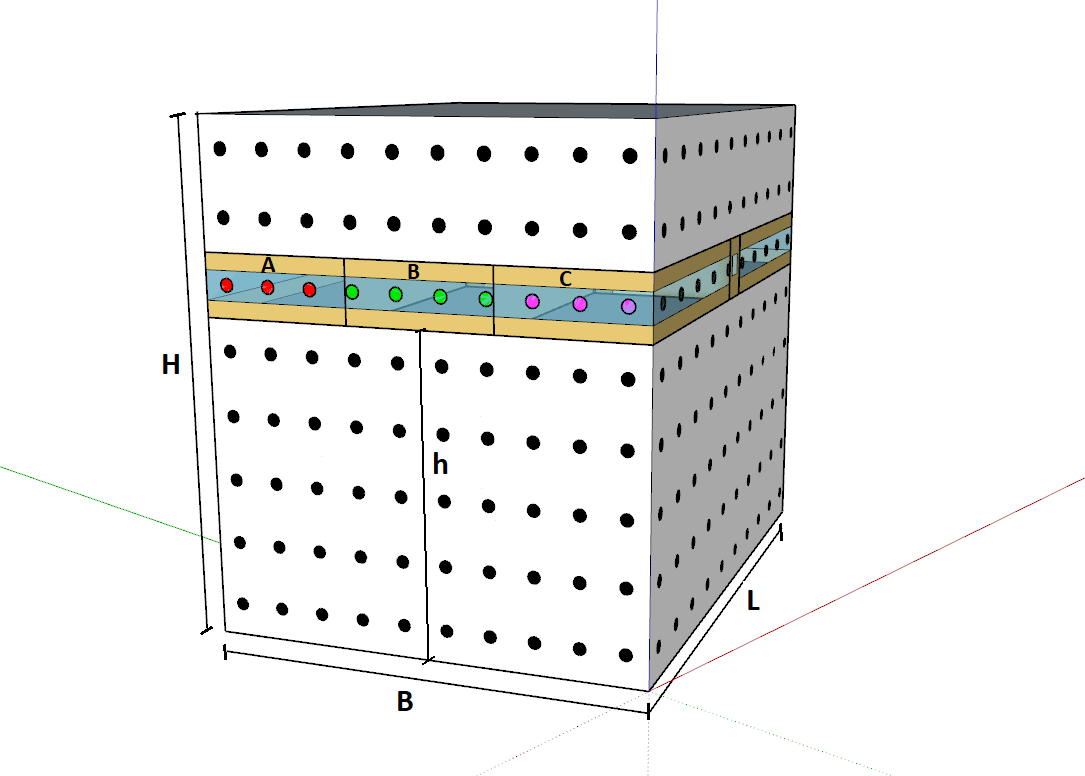
\includegraphics[width=1\linewidth]{img/ex_TPU_h.png}
	\label{fig:tpuwindows}
	%			\begin{flushleft}
	%				Fonte: \citeauthoronline{TPU2018} \cite{TPU2018}, adaptado pelo autor.
	%			\end{flushleft}
\end{figure}


\subsection{Simulação simplificada}

Nesta etapa do método, buscou-se simplificar o modelo de escritório desenvolvido no EnergyPlus, atentando-se às limitações relacionadas à simplificação do modelo.
O objetivo de gerar um metamodelo por meio de redes neurais artificiais (RNA) para se obter a EHF faz com que se busque parametrizar ao máximo as simulações no EnergyPlus.
Essa parametrização pode facilitar o desenvolvimento de amostras para a pesquisa, assim como garantir uma relação mais direta dos parâmetros de entrada com os dados de saída. 
Dentre as simplificações consideradas, estão:

\begin{itemize}
	\item cálculo do Cp através do método analítico, em vez dos valores obtidos por medições em túnel de vento pela TPU;
	\item representação dos materiais da envoltória através de duas camadas: uma camada representando a capacidade térmica, e uma camada para regular a transmitância;  %(concreto)  (objeto Material:NoMass)
	\item modelagem da zona que representa apenas um escritório, sem modelar as demais zonas térmicas da edificação. Para isso, são definidas as condições de contorno relacionadas às faces da zona correspondentes a paredes adjacentes à edificação;
	\item definição de um coeficiente de fluxo mássico de ar relacionado à infiltração de ar pela porta, e do valor do Cp relacionado a essa porta, que no modelo de uma zona está voltada para o ambiente externo, e não para a circulação.
\end{itemize}

O impacto nos resultados das simulações foram verificados para cada uma das simplificações mencionadas, a partir da análise de diversos casos amostrados pelo método de amostragem do hipercubo latino (LHS). O tamanho das amostras foi definido em relação ao tempo disponível para executar as simulações.
Finalmente, foi definida a forma mais adequada de se simplificar o modelo, assim como a margem de erro que espera-se encontrar ao assumir tais simplificações.
A seguir, cada uma dessas etapas é descrita.

%		Nem todos os parâmetros foram variados em todas as etapas deste processo. Optou-se por variar apenas os parâmetros que pudessem influenciar os resultados relacionados a cada análise. Quando não variados, os parâmtros tiveram seus valores fixados de acordo com a Tabela \ref{table:paramfix}.
%		
%		\begin{table}[h]
%			\centering
%			\caption{Parâmetros fixados na validação do modelo analítico para o cálculo do Cp.}
%			\label{table:paramfix}
%			\begin{tabular}{|c |c |}
%				\hline
%				\textbf{Parâmetro} & \textbf{Valor adotado} \\
%				\hline
%				Altura do pavimento & 15 m \\
%				\hline
%				Fator solar do vidro & 0,87 \\
%				\hline
%				Fator de abertura da janela & 1,0 \\
%				\hline
%				Capacidade térmica da parede & 155 kJ/m$^2$K \\
%				\hline
%				Absortância da parede & 0,5 \\
%				\hline 
%				Ângulo de sombreamento & 0 graus \\
%				\hline 
%			\end{tabular}
%			\begin{flushleft}
%				Fonte: o autor.
%			\end{flushleft}				
%		\end{table}
%		
%		
\subsection*{Cálculo do coeficiente de pressão pelo método analítico}

O EnergyPlus, através do AFN, possui uma opção para calcular automaticamente os Cp's para as simulações.
Quando essa opção é escolhida o programa gera apenas um Cp por fachada da edificação, e os valores podem ser obtidos por dois algorítimos diferentes: no caso de edificações altas (\textit{highrise}), utiliza-se o modelo de \citeonline{Atkins}; no caso de edificações baixas (\textit{lowrise}), utiliza-se o modelo de \citeonline{Swami1988}.
Enquanto que pelo método analítico (MA) os Cp's podem ser obtidos para quaisquer razões entre as dimensões das fachadas da edificação, os valores medidos em túnel de vento pela TPU são fornecidos para edificações com proporções entre largura, profundida e altura específicas.
Os valores de Cp para o tipo de edificação abordada neste estudo são disponibilizados pela TPU para 25 geometrias diferentes, das quais 13 são para edificações \textit{highrise}, e 12 são para edificações \textit{lowrise}.

Para verificar o quanto a fonte escolhida na definição dos Cp's influencia nos resultados das simulações, inicialmente verificou-se as diferenças entre os valores dos Cp's das medições em túnel de vento (fornecidos pela TPU), e os valores dos Cp's obtidos pelo MA (algorítimos do EnergyPlus). Para cada uma das 25 geometrias disponíveis, calculou-se a diferença entre os Cp's, de acordo com a Equação \ref{eq:Cpdiff}.

\begin{equation}
\label{eq:Cpdiff}
\overline{\Delta}_{Cp} = \frac{\sum_{i=1}^{4}{\sum_{j=0}^{11}{|\overline{Cp}^{TPU}_{f_i,\alpha_j} - Cp^{MA}_{f_i,\alpha_j}}|}}{48}
\end{equation}

Onde:

$\overline{\Delta}_{Cp}$ é igual à diferença absoluta média entre os valores dos Cp's obtidos pela base da TPU e obtidos pelo MA;

$\overline{Cp}^{TPU}_{f_i,\alpha_j}$ é igual ao valor médio dos Cp's disponibilizados pela base de dados da TPU para a fachada $i$ de uma edificação, para o ângulo de incidência do vento igual a $\alpha_j$;

$Cp^{MA}_{f_i,\alpha_j}$ é igual ao Cp calculado pelo MA para a fachada de uma edificação com proporções iguais às da fachada $i$, para o ângulo de incidência do vento igual a $\alpha_j$;

$f_i$ é a fachada $i$ da edificação avaliada;

$\alpha_j$ é o ângulo de incidência do vento  sobre a fachada, em graus, e tem valor igual a $30 \cdot j$.		
%		$\alpha_j$ é o ângulo de incidência do vento considerado sobre a fachada, que varia de 0 a 330 graus, com intervalos de 30 graus;
\\

%		Cada Cp médio ($Cp_{TPU,i,j}$), medido pela TPU em um ponto $j$ de uma fachada $i$, teve um Cp correspondente calculado pelo método analítico ($Cp_{ANALITICO, i}$), para a mesma fachada $i$. Essa subtração foi efetuada para os diferentes ângulos ($\alpha$) disponíveis na base da TPU.
%		As diferenças entre os valores dos Cp's foram calculadas obtendo-se o Cp pelo método analítico para cada fachada, de cada geometria disponível pela TPU, e subtraindo-se o valor do Cp calculado pelos valores disponibilizados pela base da TPU para a sua fachada correspondente (Equação \ref{eq:Cpdiff}).

A partir dessas diferenças entre os valores dos Cp's ($\overline{\Delta}_{Cp}$), escolheu-se a geometria com a maior diferença absoluta média como modelo base na análise da influência nos resultados das simulações no EnergyPlus.
Esta análise foi conduzida gerando-se uma amostra de 1.000 casos pelo LHS.
Os parâmetros variados e seus limites mínimos e máximos foram definidos pela metodologia do item \ref{subsec:par}, com exceção da razão entre a largura e profundidade das zonas e a altura do pavimento em relação ao solo.
A razão entre a largura e profundidade das zonas teve que ser alterada de acordo com a variação da área das salas, para se ajustar à geometria da edificação definida como modelo base da análise.
A altura do pavimento em relação ao solo também foi limitada pelas proporções da geometria escolhida para o modelo base.
Vale destacar que a base da TPU permite a obtenção de diferentes Cp's para diferentes janelas de uma mesma fachada, enquanto que nas simulações baseadas no MA, utiliza-se apenas um valor de Cp por fachada, devido à limitação do método. 
Para cada caso da amostra gerada, foram simulados um modelo com Cp’s baseados no MA, e um modelo com Cp’s baseados na base da TPU (túnel de vento).
Assim, as médias anuais das trocas de ar por hora (ACH) e a EHF foram comparadas entre as simulações.
%		com Cp's medidos em túnel de vento pela TPU, e simulações com Cp's obtidos pelos métodos analíticos padrão do EnergyPlus.

%		Para cada uma dessas geometrias disponíveis, valores de Cp são disponibilizados para diversos pontos na fachada da edificação, de acordo com a Figura \ref{fig:tpupoints}.
%		
%		\begin{figure}[h]
%			\centering
%			\caption{Exemplo do posicionamento dos pontos com valores de Cp na fachada}
%			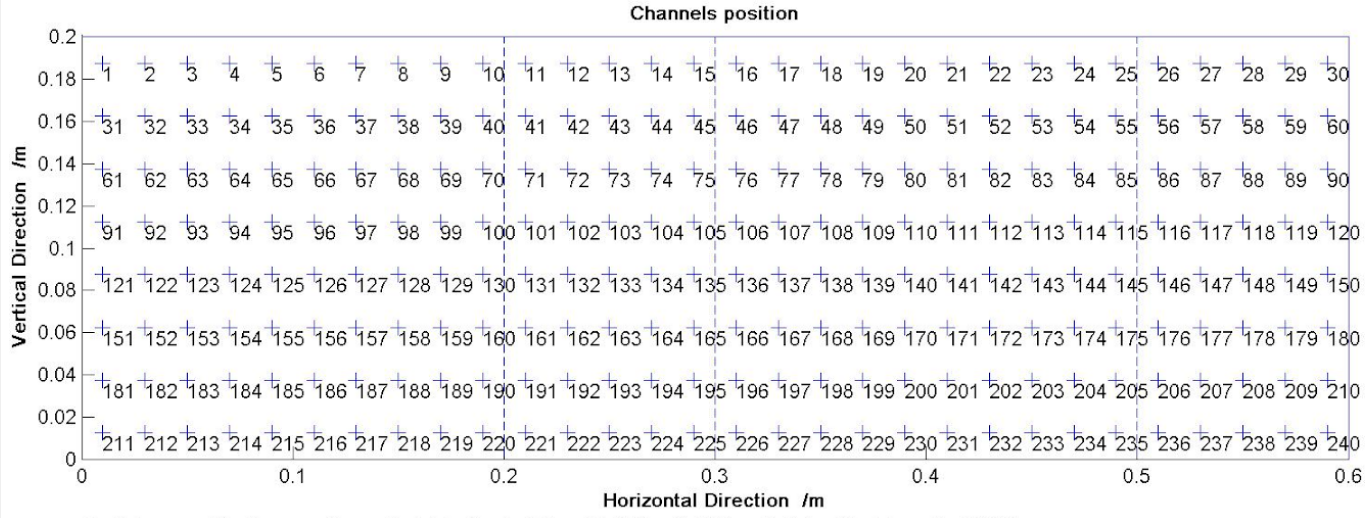
\includegraphics[width=1\linewidth]{img/tpu_points.png}
%			\label{fig:tpupoints}
%			\begin{flushleft}
%				Fonte: \citeauthoronline{TPU2018} \cite{TPU2018}, adaptado pelo autor.
%			\end{flushleft}
%		\end{figure}					

\subsection*{Representação da envoltória com duas camadas}

Para possibilitar a parametrização contínua e independente das propriedades termofísicas da envoltória, considerou-se a utilização de uma parede com propriedades equivalentes, modelada com uma camada de concreto, para representar a capacidade térmica, e uma camada modelada com o objeto \textit{Material:NoMass}, para regular a transmitância (Figura \ref{fig:parede_eq}).

\begin{figure}[h]
	\centering
	\caption{Parede equivalente}
	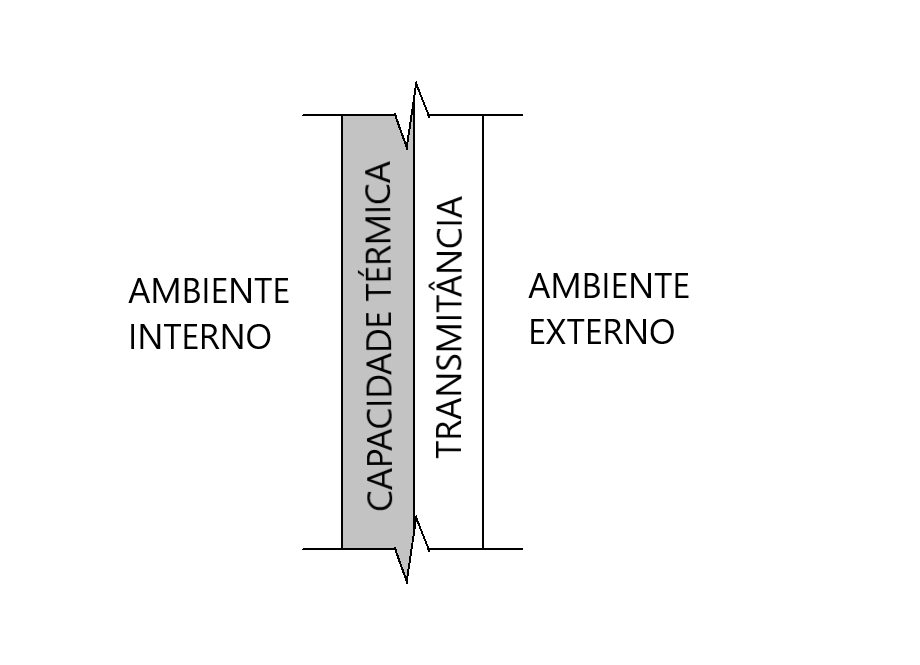
\includegraphics[width=1\linewidth]{img/parede_eq.png}
	\label{fig:parede_eq}
\end{figure}

A validação da modelagem simplificada da parede foi realizada para dois tipos de paredes referência:

\begin{itemize}
	%			\item parede de concreto;
	\item parede de gesso com lã de rocha;
	\item parede de alvenaria e reboco.
\end{itemize}

Como a modelagem da parede de alvenaria possui uma camada de ar no meio da parede, avaliou-se a possibilidade de considerar apenas a metade interna desta parede referência para definir a capacidade térmica de sua parede equivalente. Essa consideração parte do pressuposto de que a camada interna de ar faz com que a inércia térmica da metade exterior da parede não influencie consideravelmente a zona térmica analisada.

Para validar essa simplificação, gerou-se uma amostra utilizando LHS, com 100 casos.
Os parâmetros variados e seus limites mínimos e máximos foram definidos pela metodologia do item \ref{subsec:par}, com exceção da transmitância e capacidade térmica da parede.  % os parâmetros relacionados com a propriedades termofísicas da parede.	% e a absortância????
%		O modelo preliminar sofreu variação dos seguintes parâmetros: área, razão entre largura e profundidade da zona, pé-direito, azimute, absortância, PAF, taxa de ocupação. Os demais parâmtros foram fixados de acordo com a Tabela \ref{table:paramfix}.
Cada caso da amostra foi simulado com os dois tipos de paredes diferentes, e suas paredes equivalentes. No caso da parede de alvenaria, dois modelos de parede equivalente foram desenvolvidos: considerando a capacidade térmica total da parede, e considerado apenas metade da capacidade térmica.
A partir dos resultados, observou-se a diferença média entre as temperaturas operativas das zonas simuladas com as paredes referências em relação às simulações com as respectivas paredes equivalentes. O mesmo foi realizado comparando-se a EHF.

\subsection*{Condição de contorno das paredes adjacentes à edificação}

Simular apenas uma zona térmica, em vez de um edifício inteiro, ou um pavimento com diversas zonas, possibilita a simulação de casos diversos em menor tempo.
Essa consideração facilita a parametrização do modelo, e pode oferecer resultados satisfatórios se for adequadamente implementada.
A partir dessa premissa, foi desenvolvido um modelo com apenas uma zona térmica (Figura \ref{fig:singlezone}).

\begin{figure}[h]
	\centering
	\caption{Modelo de uma zona}
	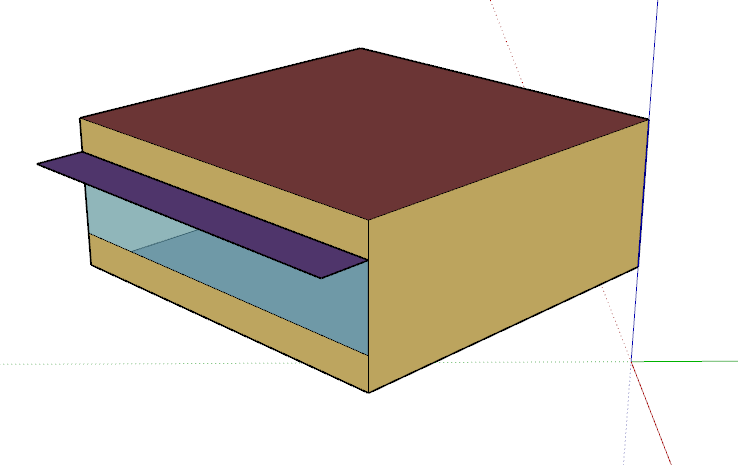
\includegraphics[width=1\linewidth]{img/model.PNG}
	\label{fig:singlezone}
\end{figure}

Para modelar essa zona, considerou-se as paredes correspondentes a superfícies voltadas para outros escritórios como adiabáticas. A superfície que representa a parede voltada para a circulação foi avaliada com duas condições de contorno: 1) como adiabática, e 2) como \textit{outdoors}, sem incidência de vento ou sol (Figura \ref{fig:adiabatic_outdoors}).	
A consideração do uso da condição \textit{outdoors} foi pela hipótese de que, sem a radiação solar direta e sem o aumento de convecção causada pelo vento, a temperatura do ar da zona da circulação (por não ter cargas internas consideráveis) poderia se manter mais próxima à temperatura do ar externo do que às das zonas das salas de escritórios.

\begin{figure}[h]
	\centering
	\caption{Modelagem com parede adiabática e \textit{outdoors}}
	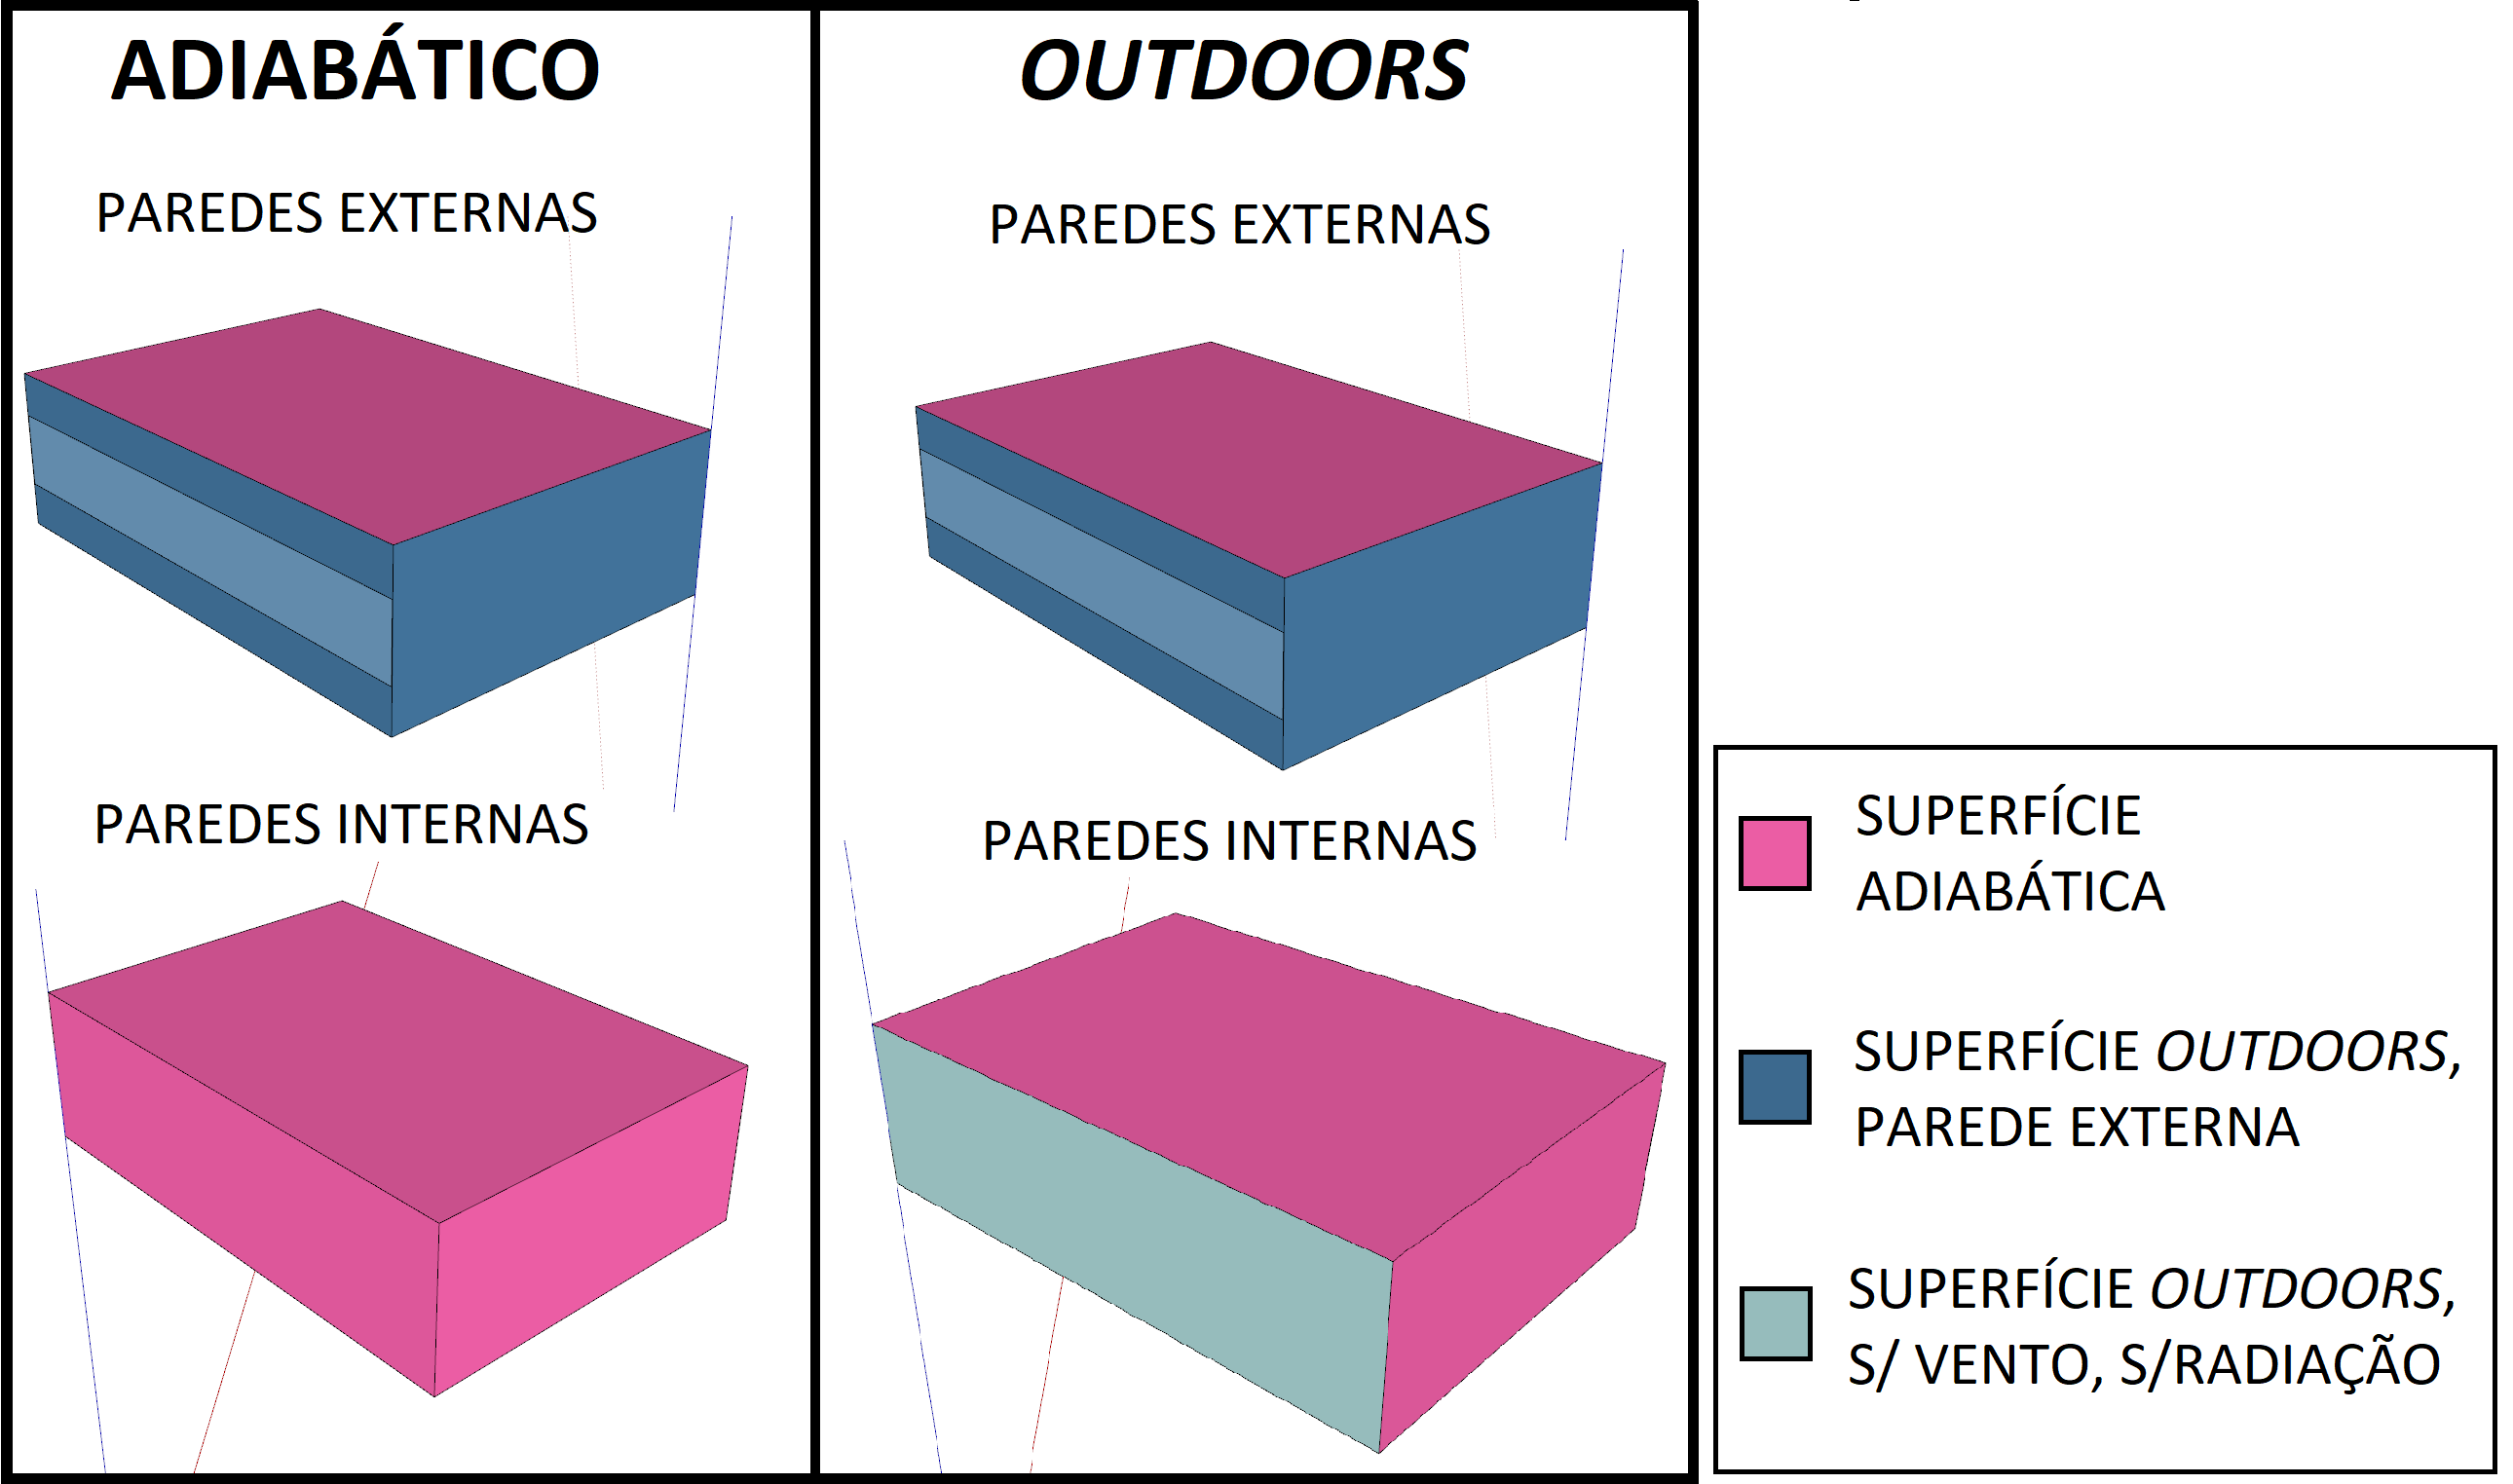
\includegraphics[width=1\linewidth]{img/adiabatic_outdoors.png}
	\label{fig:adiabatic_outdoors}
\end{figure}


A modelagem da ventilação natural sofre um impacto significativo quando o escritório é modelado como apenas uma zona térmica.
Esse impacto é devido à forma como a rede de fluxo de ar é distribuída. No caso do modelo referência, a porta é voltada para a circulação, enquanto que no caso de uma única zona térmica, a porta desta zona é voltada para o ambiente externo. 
Além disso, não é possível modelar uma porta em uma parede adiabática. Para não deixar a diferença na ventilação natural influenciar as análises comparativas entre as simulações, a ventilação natural não foi modelada para esta etapa.
Em vez disso, as simulações foram desenvolvidas com uma taxa de infiltração de ar constante durante a ocupação. O valor escolhido para a taxa de renovação de ar foi igual ao valor médio do ACH obtido na etapa da comparação entre os Cp's, que é igual a 30 ACH.

A amostra gerada pelo LHS nesta etapa foi de 100 casos.
Os parâmetros variados e seus limites mínimos e máximos foram definidos pela metodologia do item \ref{subsec:par}.
Para cada caso gerado perlo LHS, além da simulação detalhada, seis modelos de uma zona foram simulados, correspondendo a cada uma das zonas do modelo detalhado.
Para validar o uso de diferentes condições de contorno, comparou-se os resultados de EHF e temperaturas operativas das simulações de uma zona térmica com os resultados obtidos para as zonas térmicas das simulações detalhadas.
A condição de contorno com menores diferenças médias absolutas, de temperatura operativa e EHF, foi escolhida para se conduzir as simulações simplificadas.

\subsection*{Modelagem da ventilação natural na simulação simplificada}

A modelagem da ventilação natural na simulação simplificada deve ser adaptada para se ter resultados correspondentes ao esperado em relação à simulação detalhada, pois enquanto a rede de fluxo de ar na simulação detalhada é modelada de acordo com a Figura \ref{fig:AFN_ref}, na simulação simplificada essa rede é modelada de acordo com a Figura \ref{fig:AFN_sz}.	

\begin{figure}[h]
	\centering
	\caption{Rede de fluxo de ar na simulação referência}
	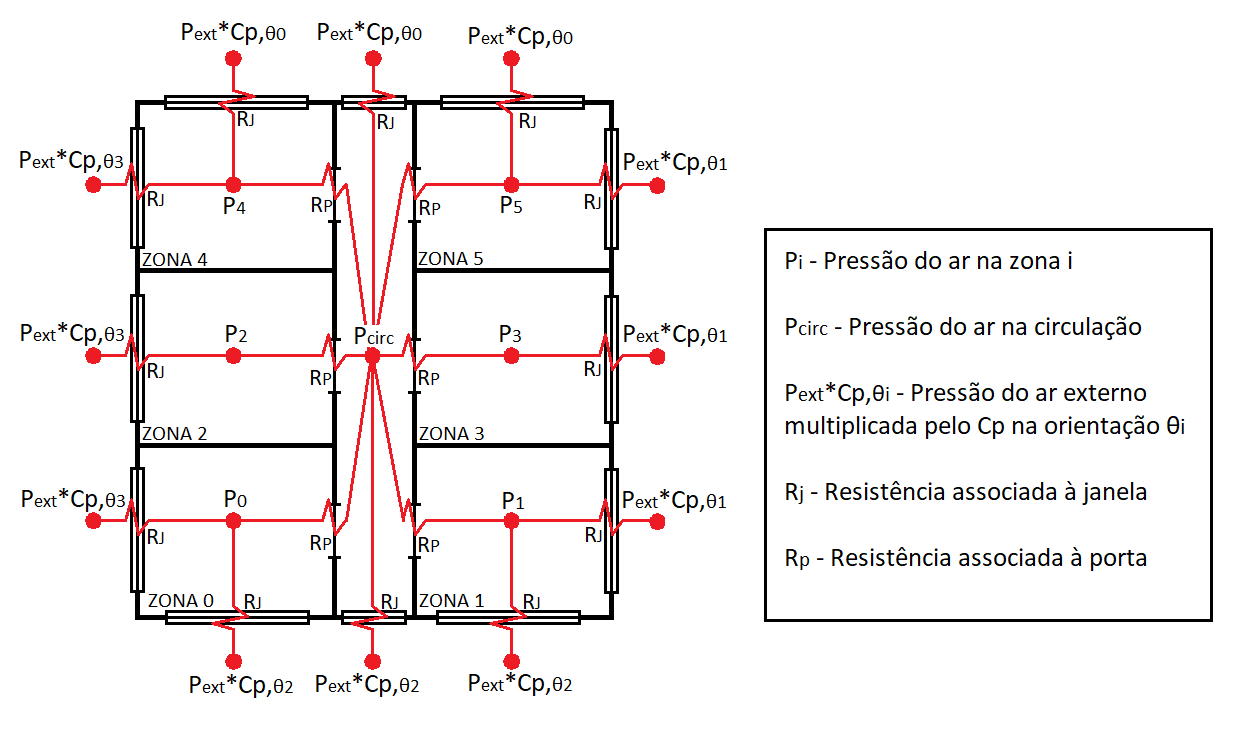
\includegraphics[width=1\linewidth]{img/AFN_ref.png}
	\label{fig:AFN_ref}
\end{figure}	

\begin{figure}[h]
	\centering
	\caption{Rede de fluxo de ar na simulação simplificada}
	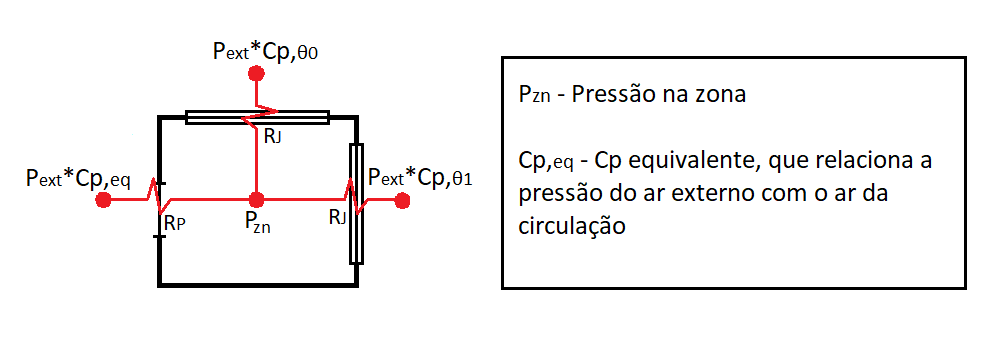
\includegraphics[width=1\linewidth]{img/AFN_sz.png}
	\label{fig:AFN_sz}
\end{figure}
%		As limitações desta adaptação e as formas de contorná-las serão explicadas neste item.

A proposta para contornar esse problema foi desenvolvida a partir da hipótese de que, na simulação simplificada, seria possível criar um Cp associado à porta ($Cp_{eq}$), capaz de descrever as diferenças de pressão de ar entre a circulação e a sala.  % , para cada ângulo de vento.

Quando o objeto \textit{AirflowNetwork:MultiZone:Component: DetailedOpening} é utilizado, o cálculo do fluxo de ar entre dois pontos é feito pela Equação \ref{eq:AFEDOP_opened}, se a porta/janela está aberta, ou pela Equação \ref{eq:AFEDOP_closed}, que é utilizada para calcular a infiltração de ar quando a abertura está fechada.

\begin{equation}
\label{eq:AFEDOP_opened}
\dot{m}_{i,j} = C_d \Theta 	\int_{z=0}^{z=H} \sqrt{2 \rho (P_{i(z)} - P_{j(z)})} W d_z 
\end{equation}

\begin{equation}
\label{eq:AFEDOP_closed}
\begin{split}
\dot{n}_{i,j} = C_q [2\int_{z=0}^{z=H} {(P_{i(z)} - P_{j(z)})}^{exp} d_z + \\ W{(P_{i(0)} - P_{j(0)})}^{exp} + W{(P_{i(H)} - P_{j(H)})}^{exp}]
\end{split}
\end{equation}

Onde:

$\dot{m}_{i,j}$ é o fluxo de ar entre os pontos $i$ e $j$, quando a porta/janela está aberta (kg/s);

$C_d$ é o coeficiente de descarga da abertura (-);

$\Theta$ é a fração de abertura (-);

$H$ é a altura da abertura (m);

$\rho$ é a densidade do ar (kg/m$^{3}$);

$P_{i(z)}$ é a pressão de ar no ponto $i$, altura $z$ (Pa);

$W$ é a largura da abertura (m);

$\dot{n}_{i,j}$ é o fluxo de ar entre os pontos $i$ e $j$, quando a porta/janela está fechada (kg/s);

$C_q$ é o coeficiente de fluxo mássico de ar da abertura (-);

$exp$ é o expoente de fluxo de massa de ar (-).
\\

As seguintes condições de contorno foram estabelecidas para facilitar o cálculo do $Cp_{eq}$:
\begin{itemize}			 
	\item o valor do $exp$ foi definido como 0,5;
	\item o valor de $\rho$ foi definido sempre como 1,200 kg/m$^3$;
	\item os fluxos de ar foram considerados como unidimensionais, portanto os valores de $P$ não variaram com o a altura ($z$);
	\item O valor do $Cp_{eq}$ foi definido assumindo-se que as janelas estariam com sua máxima fração de abertura ($\Theta$).
\end{itemize}

Em cada \textit{timestep}, a soma dos fluxos de ar que entram e saem de uma zona $i$ é igual a zero. Assumindo-se as condições de contorno descritas, a pressão de ar em cada zona térmica pode ser estimada pela Equação \ref{eq:P}. Dessa forma é possível encontrar a relação entre as pressões de ar de todas as zonas da simulação de referência.

\begin{equation}\label{eq:P}
%\resizebox{\linewidth}{!}{
\begin{split}
P_{zn} = \frac{\sum_{i=1}^{N_P}{P_{i} (C_q L_i)^2} +  %\\
	\sum_{j=1}^{N_J}{P_{ext} C_{p,j} 2 \rho (C_{d} \Theta_j A_j)^2 }}
{\sum_{i=1}^{N_P}{(C_q L_i)^2} +  %\\
	\sum_{j=1}^{N_J}{2 \rho (C_{d} \Theta_j A_j)^2 }}
\end{split}
%}
\end{equation}

Onde:

$P_{zn}$ é a pressão do ar na zona analisada (Pa);

$N_P$ é igual ao número de portas que se conectam à zona (-);

$P_i$ é a pressão de ar na zona ligada pela porta $i$ (Pa);

$L_i$ é igual ao perímetro da porta $i$ (m);

$N_J$ é igual ao número de janelas que se conectam à zona (-);

$P_{ext}$ é a pressão do ar no ambiente externo (Pa);

$C_{p,j}$ é o Cp na superfície da janela $j$ (-);

$A_j$ é igual à área da janela $j$ (m$^2$).
\\

Finalmente, os Cp's equivalentes ($Cp_{eq}$) foram definidos calculando-se a relação entre a pressão de ar na zona da circulação e a pressão do ar no ambiente externo, para cada direção angular do vento, de acordo com a Equação \ref{eq:Cpeq}.

\begin{equation}\label{eq:Cpeq}
Cp_{eq,\alpha} = \frac{P_{circ}}{P_{ext}}
\end{equation}

Onde:

$P_{circ}$ é a pressão de ar na circulação;

$Cp_{eq,\alpha}$ é igual ao Cp equivalente na abertura da porta, para um ângulo de vento $\alpha$.
\\

Outra limitação relacionada à VN na simulação simplificada é o fato de que o AFN do EnergyPlus não permite modelar aberturas ou qualquer tipo de infiltração de ar em superfícies adiabáticas. Para contornar esse problema, no caso de se modelar uma parede voltada para a circulação como adiabática, é possível associar a infiltração referente à porta a uma outra superfície da zona.  %  que esteja voltada para o ambiente externo 
Isso se faz possível no momento em que se calcula diretamente os coeficientes de pressão (Cp's) dos nós relacionados às aberturas da zona térmica.
Desta forma define-se o Cp para uma superfície (seja janela ou parede), considerando-se qualquer orientação desejada, e não necessariamente a orientação definida para esta superfície pela geometria do modelo.		
A modelagem do fluxo de ar pelas portas dos escritórios nas simulações simplificadas foi desenvolvida com o objeto \textit{AirflowNetwork:MultiZone:Surface:Crack}. O motivo para se utilizar este objeto é porque este é um objeto que pode ser associado a qualquer tipo de superfície. Portanto, o objeto do \textit{crack} foi associado sempre à parede externa oposta à parede que estaria voltada para a circulação, como apresentado na Figura \ref{fig:AFN_crack}.

\begin{figure}[h]
	\centering
	\caption{Solução para infiltração de ar entre a zona e a circulação}
	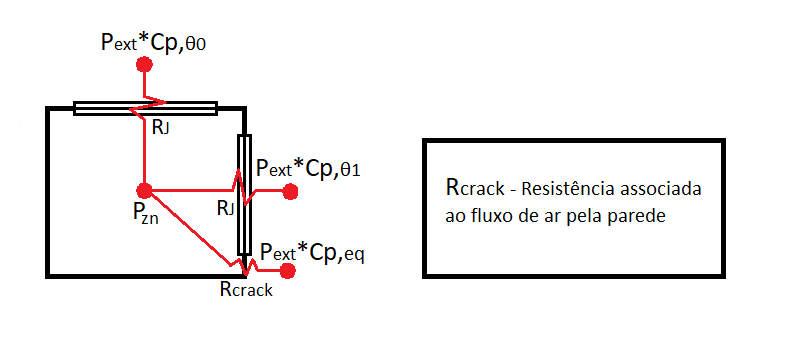
\includegraphics[width=1\linewidth]{img/AFN_crack.png}
	\label{fig:AFN_crack}
\end{figure}	

Devido a essas considerações, a validação nesta etapa foi conduzida para duas condições: utilizando-se o Cp calculado diretamente pelo método analítico, e utilizando-se o $Cp_{eq}$.		
Estas análises foram conduzidas considerando-se diferentes valores de coeficiente de fluxo mássico de ar para o \textit{crack}, para ajustar o valor mais adequado à taxa de infiltração que se obtém no modelo referência. Os valores considerados foram: 0,10; 0,30; 0,40; 0,45; 0,50; 0,55; 0,6; 0,7; 0,80; e 0,90 kg/s em 1 Pa.
Uma amostra de 200 casos foi gerada por LHS.
Os parâmetros variados e seus limites mínimos e máximos foram definidos pela metodologia do item \ref{subsec:par}.
Para cada caso, gerou-se uma simulação referência, mais dez simulações simplificadas. Essas dez simulações devem-se a consideração dos dois métodos para se obter os Cp's, mais os dez valores de coeficiente de fluxo mássico de ar analisados. As comparações foram efetuadas observando-se os resultados de ACH médios e EHF. 
%Como as taxas de infiltração são influenciadas pela temperatura do ar, as comparações com os modelos referências foram feitas considerando-se diferentes faixas de temperatura.

\section{Análise de sensibilidade}

Após definir como seriam gerados os modelos para as simulações simplificadas, uma análise de sensibilidade (AS) foi aplicada. Através da AS, a influência dos diferentes dados de entrada variados nas simulações foi avaliada. Com base nos resultados da AS, parâmetros não relevantes nos resultados de temperatura operativa e, consequentemente, fração de horas de desconforto por calor (EHF), foram determinados com valores fixos. Desta forma, o metamodelo foi desenvolvido considerando-se apenas parâmetros com influência expressiva nos dados de saída desejados.

O método de \citeauthoronline{Sobol1993} \cite{Sobol1993} foi utilizado para a AS, pois permite a identificação de parâmetros influentes, mesmo para casos onde a relação entre as entradas e saídas dos modelos são não-monotônicas e apresentam efeitos colineares.

A AS foi aplicada por meio de programação, utilizando-se a biblioteca \textit{SALib} \cite{Herman2017}, escrita na linguagem \textit{Python} \cite{Python}.
Os casos simulados para conduzir a AS foram amostrados pelo método de amostragem específico da AS de Sobol, pelo qual gerou-se uma amostra de 155.648 casos.
Os parâmetros variados e seus limites mínimos e máximos foram definidos pela metodologia do item \ref{subsec:par}. 
%, que gera uma sequência quasi-randômica de baixa discrepância.é uma é feita a partir de uma amostra desenevolvida específica para essa análise é definida pelo próprio método, pela qual gerou-se 99.978 casos.		
A partir dos dados de entrada de cada caso, e dos valores de EHF's resultantes das simulações termoenergéticas, obteve-se índices de sensibilidade para análise de primeira ordem, segunda ordem, e efeitos totais.

\section{Desenvolvimento do metamodelo}

O metamodelo foi desenvolvido por meio de redes neurais artificiais (RNA).		
A maneira como se descreve as variáveis de entrada dos modelos simulados para o metamodelo a ser desenvolvido pode influenciar na sua precisão e na representação adequada dos fenômenos termofísicos.
Portanto, no processo de definição das variáveis de entrada do metamodelo, busca-se a melhor forma de descrever as diversas características das zonas térmicas.
Esse é um processo iterativo, que envolve diferentes variáveis, utilizando-se transformações, normalizações e funções destas. 
É importante também observar os hiperparâmetros (parâmetros relacionados ao processo de aprendizagem automática) escolhidos no desenvolvimento da RNA. 
A precisão dos resultados obtidos pela RNA pode depender do número de nós, número de camadas, taxa de aprendizagem, número de iterações, assim como outros parâmetros definidos durante o processo de treinamento. 

Ao longo do processo de desenvolvimento do metamodelo, RNA's com diferentes configurações foram testadas, utilizando-se diferentes maneiras de descrever as variáveis de entrada, e diferentes combinações de hiperparâmetros.
A base de dados utilizada para o treinamento do metamodelo foi gerada a partir de 20.000 simulações, amostrados pelo método de amostragem do LHS. %100.000 simulações, amostrados pelo método de amostragem de Sobol.
A amostra utilizada para validação foi composta por 5.000 casos, geradas por LHS.
% O motivo para se utilizar diferentes métodos de amostragem é para evitar qualquer enviesamento possivelmente relacionado ao método de amostragem.
Em ambas as amostras, os parâmetros variados tiveram seus limites mínimos e máximos definidos de acordo com o item \ref{subsec:par}, com excessão daqueles parâmetros que tiveram seus valores determinados como fixos na etapa da AS.
Os indicadores de precisão utilizados foram o erro absoluto médio e o erro absoluto do $95^{\circ}$ percentil.
É comum se utilizar a raiz quadrada do erro quadrático médio (RMSE), ou o coeficiente de determinação (R$^2$) como indicadores de desempenho. Contudo, considerando-se que o dado de saída do metamodelo será uma fração (EHF) com valor entre zero e um, o erro absoluto já é consequentemente um erro relativo. Portanto, conclui-se que o erro absoluto médio, associado ao erro absoluto $95^{\circ}$ percentil, pode estimar de maneira mais adequada a imprecisão esperada para os resultados do metamodelo.

A RNA com os melhores indicadores de precisão na etapa de treinamento foi escolhida para ter seu desempenho analisado com uma amostra de teste. 
A amostra de teste foi utilizada para verificar o desempenho da RNA quando os valores dos parâmetros determinados como fixos na etapa da AS variam. Para isso, utilizou-se a mesma amostra gerada para etapa da AS, pois as simulações já estavam finalizadas, e os casos eram diferentes daqueles utilizados no desenvolvimento da RNA.
Ao analisar os indicadores de precisão da RNA em relação às amostras de validação e de teste, o metamodelo final foi definido.

\chapter{Resultados e Discussões}
\label{chapter:Resultados}

\section{Parâmetros de entrada}
Ao analisar o banco de dados disponibilizado, obteve-se as distribuições de ocorrência em relação aos parâmetros observados (Figura \ref{fig:db_hist}).

\begin{figure}[H]
	\captionof{figure}{Distribuições de ocorrência}
	\label{fig:db_hist}
	\centering
	\begin{minipage}{.5\textwidth}
		\centering
		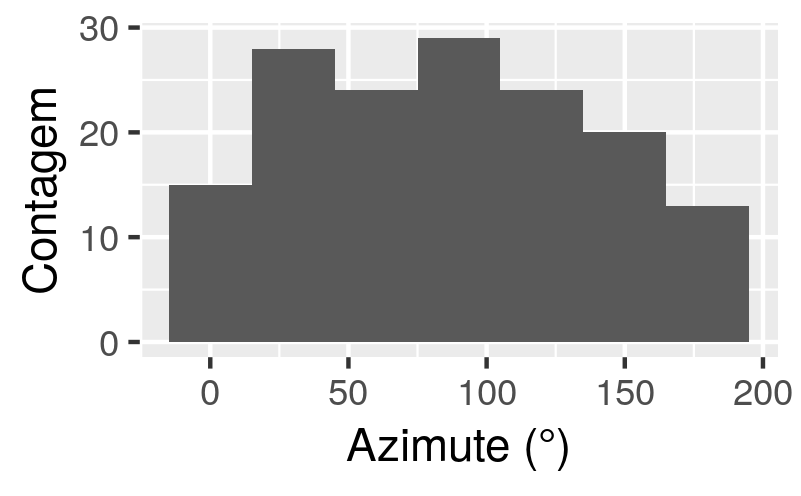
\includegraphics[width=\linewidth]{img/hist_azimute.png}
	\end{minipage}%
	\begin{minipage}{.5\textwidth}
		\centering
		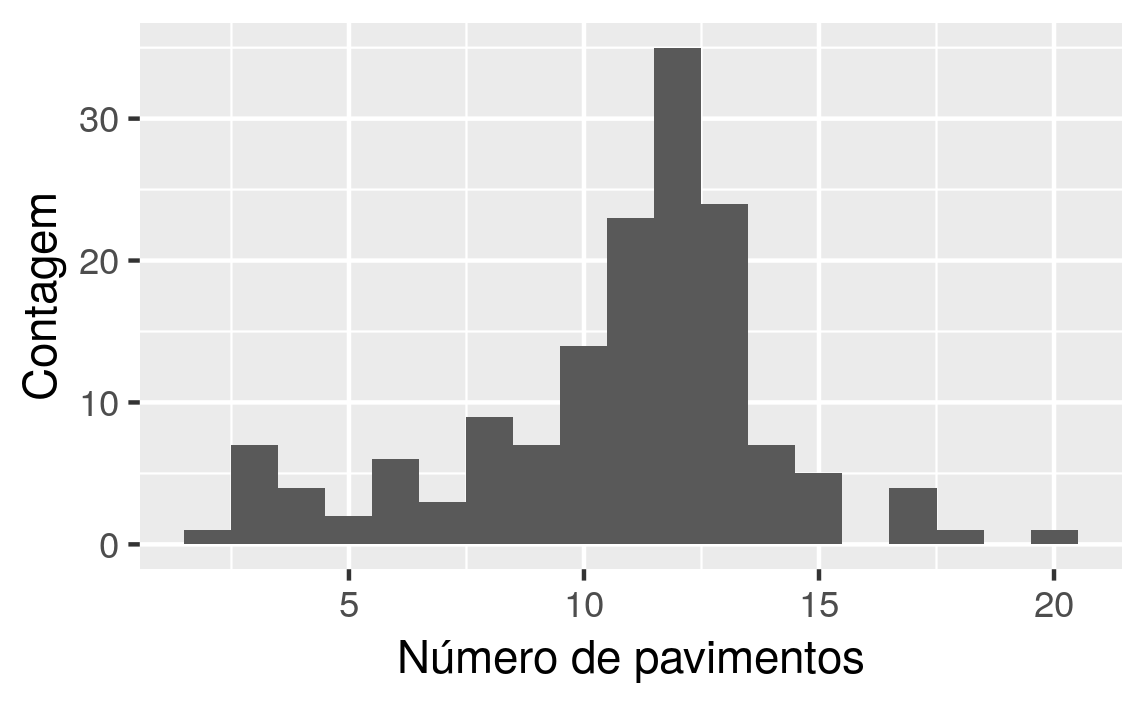
\includegraphics[width=\linewidth]{img/hist_numero_pavimentos.png}
	\end{minipage}
	\centering
	\begin{minipage}{.5\textwidth}
		\centering
		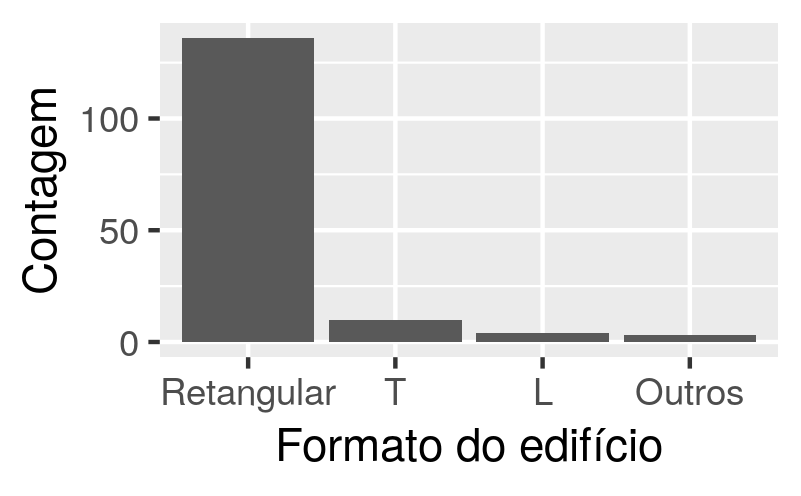
\includegraphics[width=\linewidth]{img/hist_formato.png}
	\end{minipage}%
	\begin{minipage}{.5\textwidth}
		\centering
		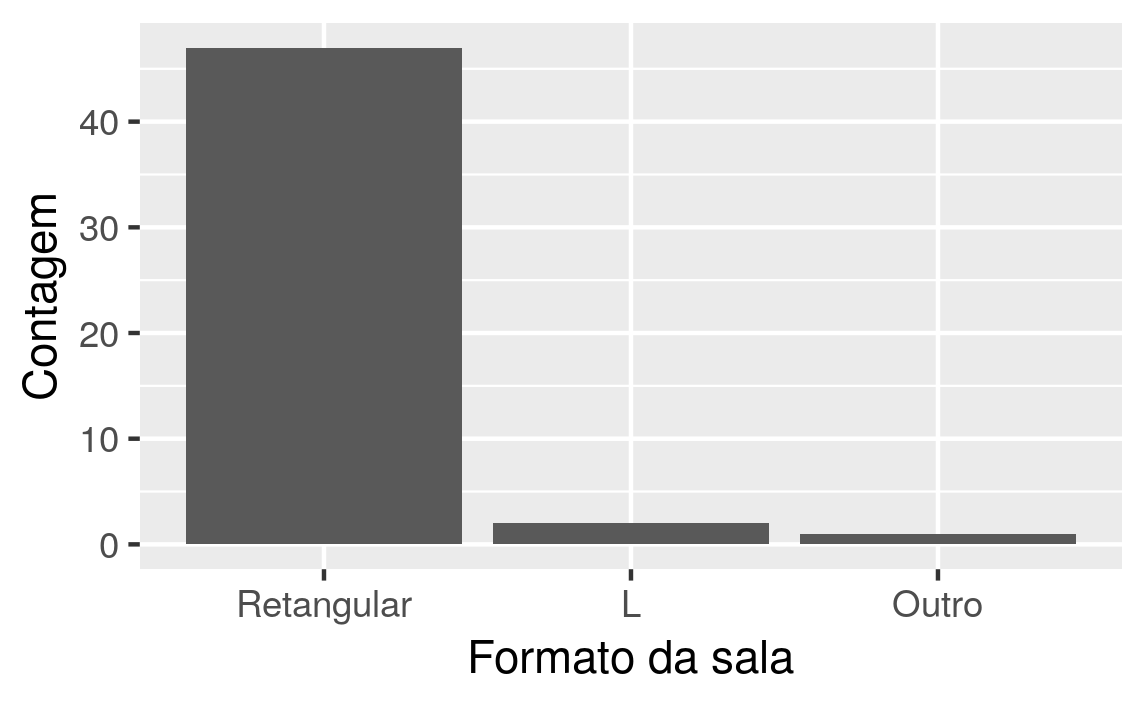
\includegraphics[width=\linewidth]{img/hist_formato_sala.png}
	\end{minipage}
	\centering
	\begin{minipage}{.5\textwidth}
		\centering
		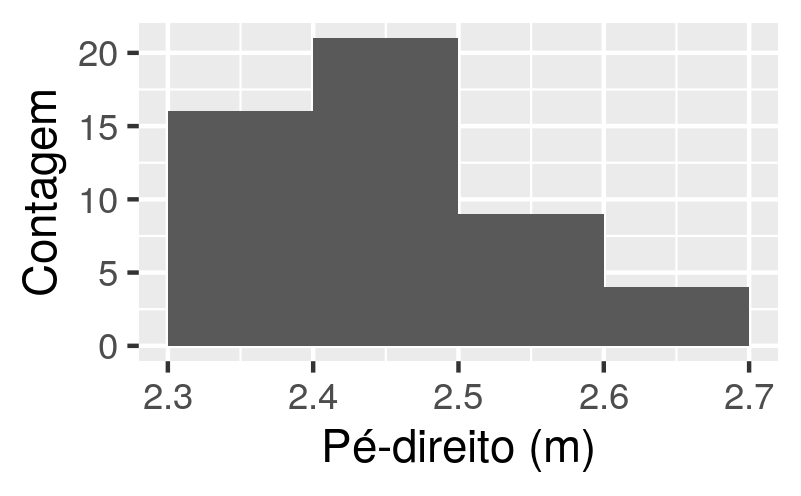
\includegraphics[width=\linewidth]{img/hist_pe_direito.png}
	\end{minipage}%
	\begin{minipage}{.5\textwidth}
		\centering
		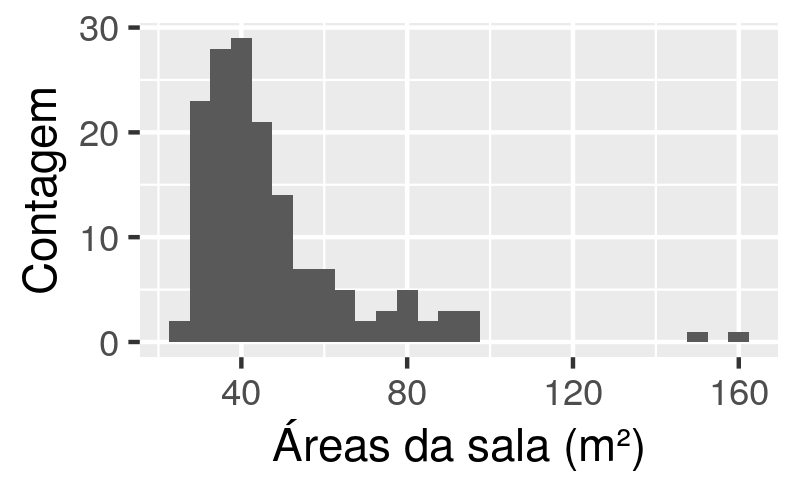
\includegraphics[width=\linewidth]{img/hist_area_zonas.png}
	\end{minipage}
	\centering
	\begin{minipage}{.5\textwidth}
		\centering
		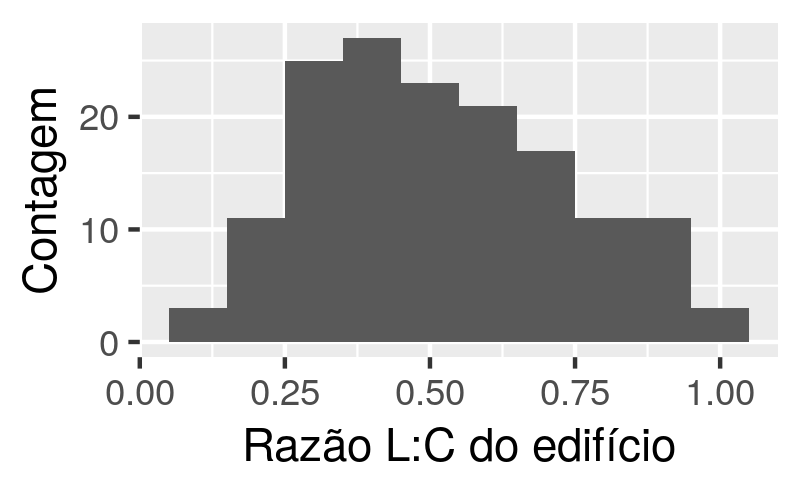
\includegraphics[width=\linewidth]{img/hist_ratio_edificio.png}
	\end{minipage}%
	\begin{minipage}{.5\textwidth}
		\centering
		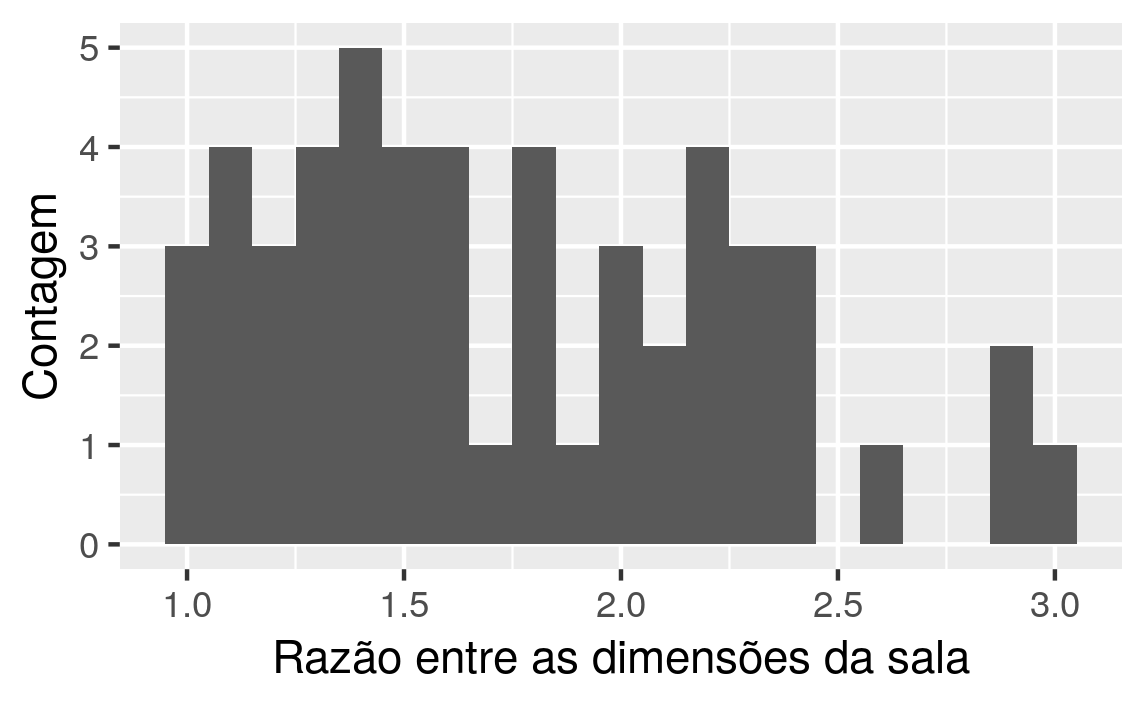
\includegraphics[width=\linewidth]{img/hist_ratio_sala.png}
	\end{minipage}
\end{figure}
\begin{figure}
	\ContinuedFloat
	\caption[]{\textit{Continuação}} % {figure}
	\centering	
	\begin{minipage}{.5\textwidth}
		\centering
		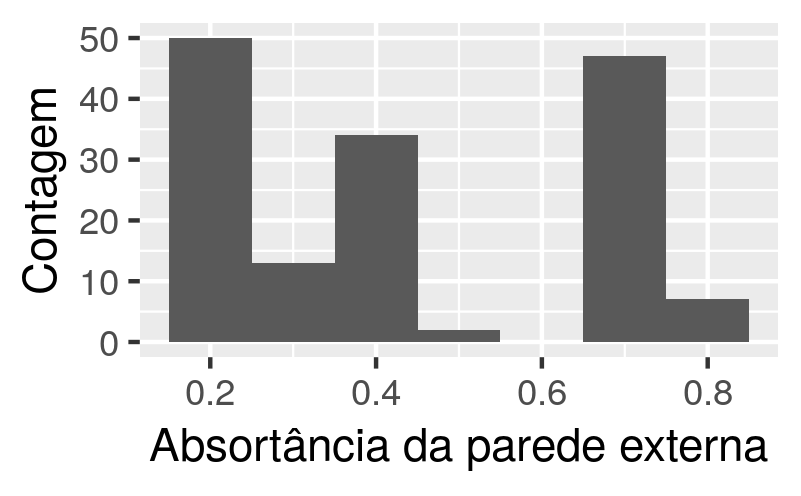
\includegraphics[width=\linewidth]{img/hist_absortancia.png}
	\end{minipage}%
	\begin{minipage}{.5\textwidth}
		\centering
		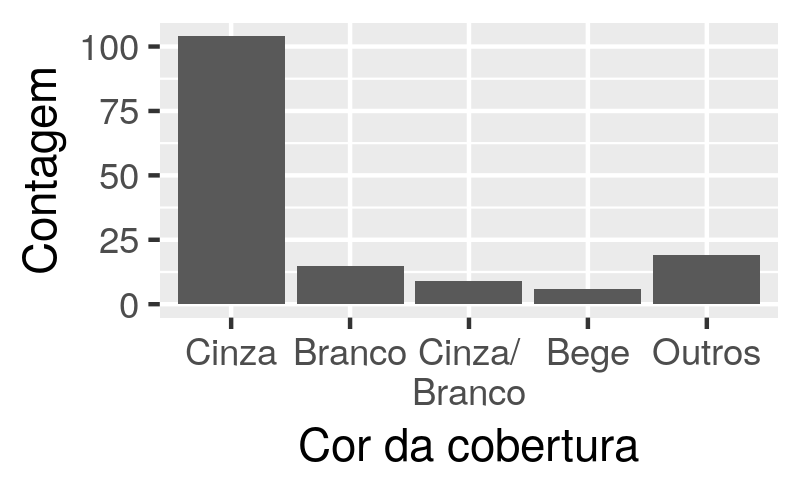
\includegraphics[width=\linewidth]{img/hist_cor_cobertura.png}
	\end{minipage}
	\centering	
	\begin{minipage}{.5\textwidth}
		\centering
		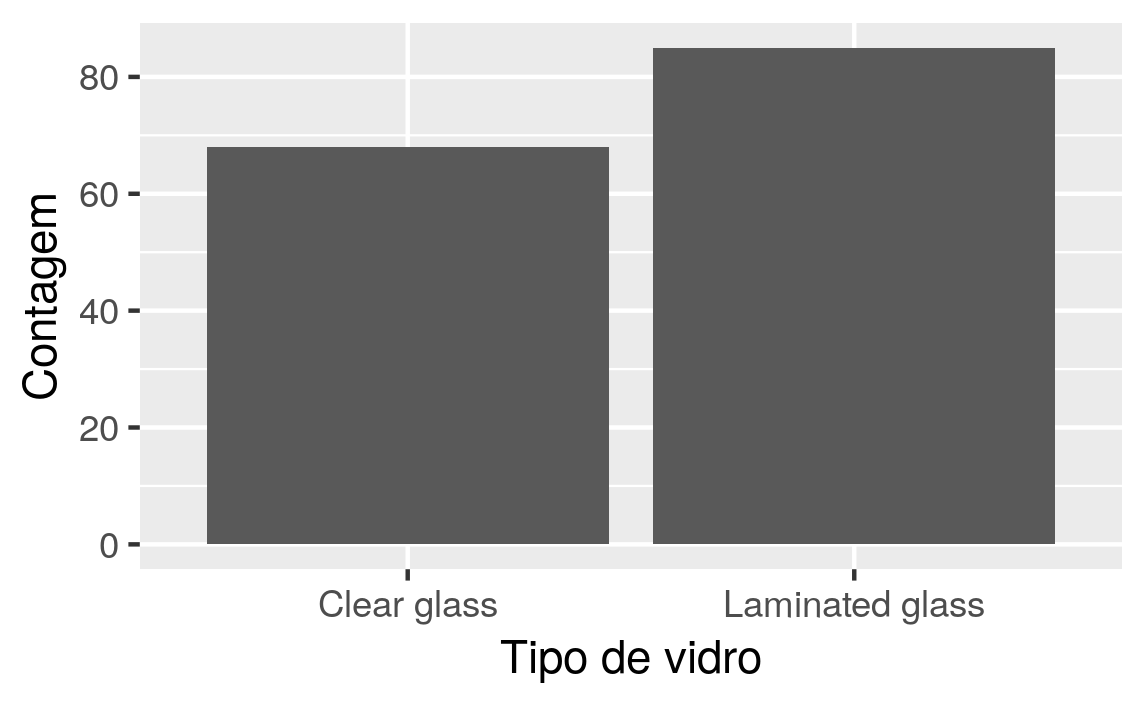
\includegraphics[width=\linewidth]{img/hist_tipo_vidro.png}
	\end{minipage}%
	\begin{minipage}{.5\textwidth}
		\centering
		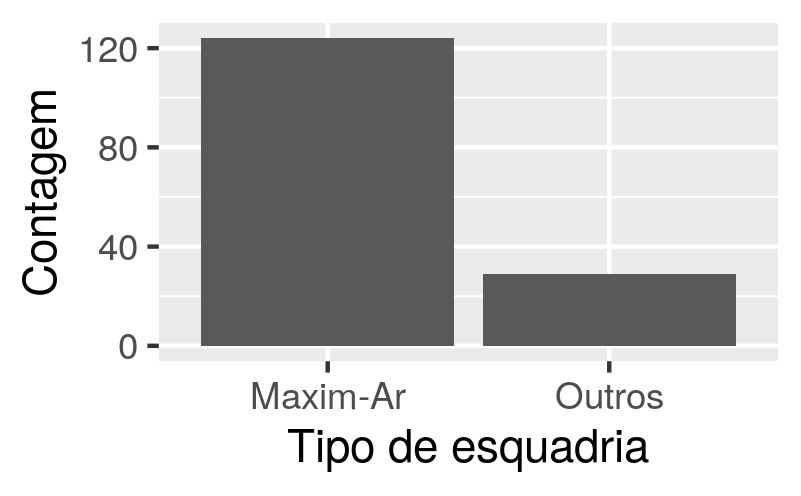
\includegraphics[width=\linewidth]{img/hist_esquadria.png}
	\end{minipage}
	\centering	
	\begin{minipage}{.5\textwidth}
		\centering
		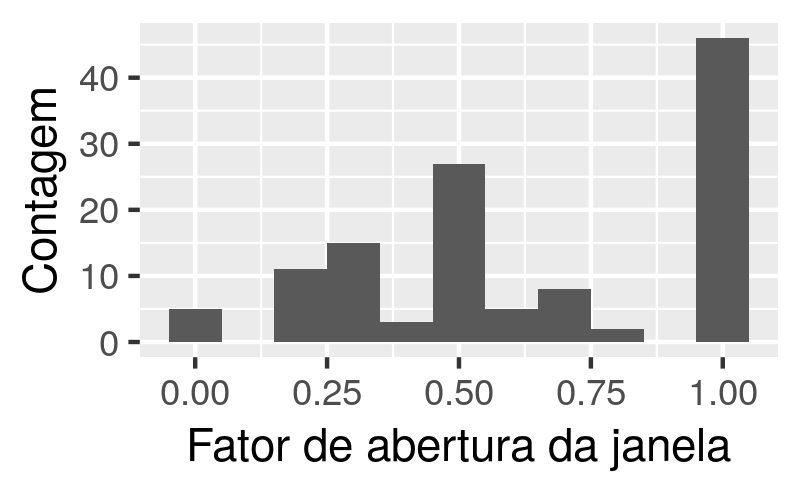
\includegraphics[width=\linewidth]{img/hist_openfac.png}
	\end{minipage}%
	\begin{minipage}{.5\textwidth}
		\centering
		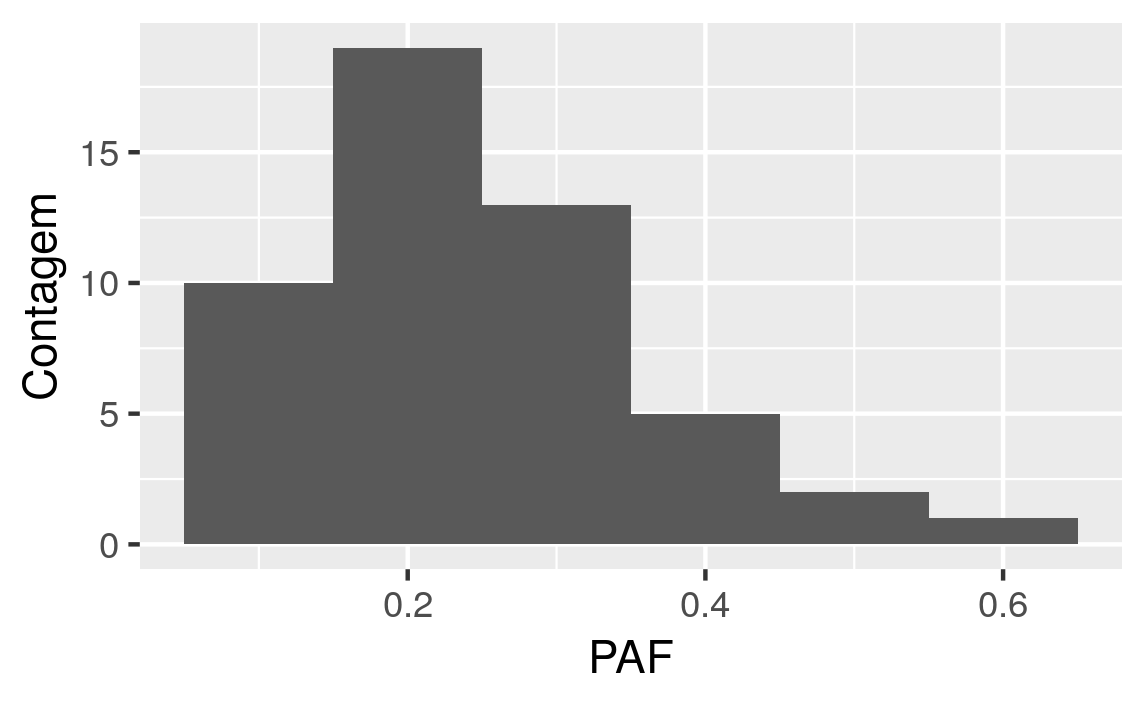
\includegraphics[width=\linewidth]{img/hist_PAF.png}
	\end{minipage}
	\centering	
	\begin{minipage}{.5\textwidth}
		\centering
		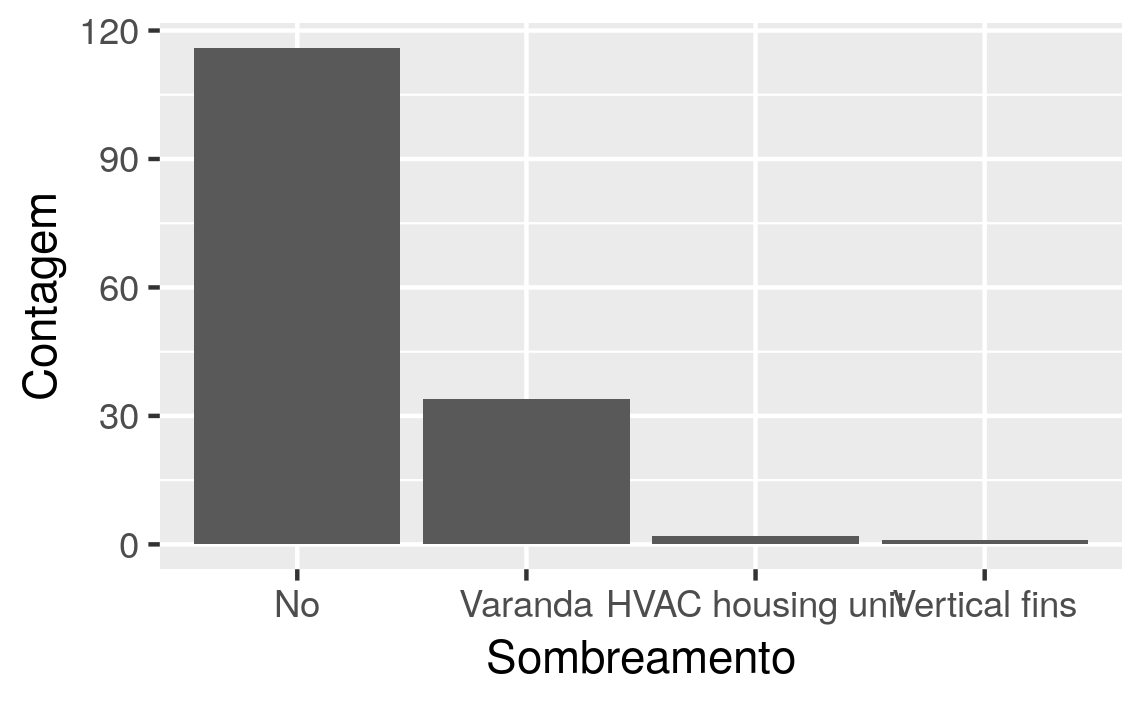
\includegraphics[width=\linewidth]{img/hist_sombreamento.png}
	\end{minipage}%
	\begin{minipage}{.5\textwidth}
		\centering
		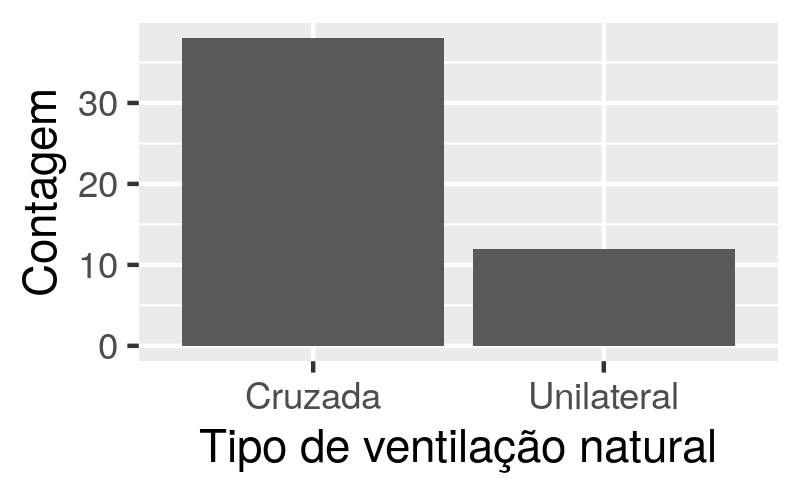
\includegraphics[width=\linewidth]{img/hist_tipo_vn.png}
	\end{minipage}
\end{figure}

Tanto os edifícios, quanto as salas existentes no banco de dados apresentam predominantemente formato retangular, a partir do qual considera-se que definir as simulações baseando-se em modelos de edificações retangulares, com salas retangulares, representa adequadamente as tipologias de edifícios encontradas na cidade de São Paulo.
A absortância da cobertura foi definida com o valor fixo de 0,7, valor aproximado para uma cobertura de cor cinza.

Observou-se que esquadrias do tipo maxim-ar são predominantes. Os objetos do \textit{Airflow Network} não modelam especificamente este tipo de esquadria. Porém, optou-se por considerar as janelas como não pivotantes. Considerar uma janela como horizontalmente pivotante implicaria na consideração de que a abertura acontece simultaneamente em cima e embaixo da janela. No caso da janela maxim-ar, por mais que a abertura aconteça em um eixo horizontal, apenas a parte inferior da janela abre.

O uso de elementos de sombreamento é pouco explorado nas edificações existentes. De qualquer maneira, considerou-se a modelagem de sombreamento horizontal sobre as aberturas da edificação, por considerar o potencial do sombreamento para bloquear a entrada de radiação nas zonas térmicas simuladas. Esse parâmetro foi variado a partir do ângulo de sombreamento formado entre a base da abertura e a proteção solar, localizada no topo da abertura.	
A maioria das salas observadas possuem ventilação cruzada, mas a ventilação unilateral é uma estratégia com ocorrência considerável.

As informações relacionadas ao tipo de vidro não permitem definir valores relacionados ao fator solar (FS). Observa-se apenas a ocorrência de vidros laminados e vidro comum incolor. Optou-se por variar o fator solar dos vidros nas simulações para avaliar o impacto deste parâmetro nos resultados de conforto térmico.

%	Os demais parâmetros observados tiveram suas distribuições variando continuamente de acordo com as distribuições obtidas. 
Como as simulações de referência foram modeladas como pavimentos da edificação, o parâmetro relacionado ao número de pavimento das edificações foi transformado no parâmetro "altura do pavimento".

A Tabela \ref{table:param_def} apresenta os limites mínimos e máximos atribuídos aos diferentes parâmetros contínuos variados nas simulações, assim como os parâmetros variados pela lógica "sim/não". A velocidade do ar foi variada com valores discretos, de acordo com a Tabela \ref{table:var} do Capítulo \ref{chapter:metodologia}.

\begin{table}[H]
	\centering
	\caption{Limites mínimos e máximos dos parâmetros}
	\label{table:param_def}
	\begin{tabular}{|l |r |}
		\hline
		\textbf{Parâmetro} & \textbf{Valores} \\
		\hline
		Área da sala (m$^2$) & 20 - 100 \\
		\hline
		Razão L:C da sala (-) & 0,4 - 2,5 \\
		\hline
		Pé-direito (m) & 2,3 - 3,2 \\
		\hline
		Azimute ($^{\circ}$) & 0 - 360 \\
		\hline
		Altura do pavimento (m) & 0 - 50 \\
		\hline 
		Absortância da parede (-) & 0,2 - 0,8 \\
		\hline 
		Transmitância da parede (W/m$^2$K) & 0,5 - 4,4 \\
		\hline 
		Capacidade térmica da parede (kJ/m$^2$K) & 0,22 - 450,00 \\
		\hline 
		PAF (-) & 0,1 - 0,6 \\
		\hline 
		Fator solar do vidro (-) & 0,20 - 0,87 \\
		\hline 
		Sombreamento ($^{\circ}$) & 0 - 80 \\
		\hline 
		Densidade de ocupação (pessoa/m$^2$) & 0,05 - 0,20 \\
		\hline 
		Fator de abertura da janela (-) & 0,2 - 1,0 \\
		\hline 
		Razão L:C do edifício (-) & 0,2 - 1,0 \\
		\hline 
		Cobertura exposta & Sim / Não\\
		\hline 
		Piso exposto & Sim / Não\\
		\hline 
		Ventilação & Cruzada / Unilateral\\
		\hline 
		Velocidade do ar (m/s) & 0,0 - 1,2 \\
		\hline 
	\end{tabular}
	%			\begin{flushleft}
	%				Fonte: \citeauthoronline{INIC} \cite{INIC}, adaptado pelo autor.
	%			\end{flushleft}				
\end{table}

\section{Simulações simplificadas}

\subsection{Cálculo do coeficiente de pressão pelo método analítico}

Ao comparar os valores dos coeficientes de pressão (Cp’s) das medições em túnel de vento da Universidade Politécnica de Tóquio (TPU) e os valores dos Cp’s obtidos pelo método analítico (MA), obteve-se um gráficos de pontos. 
A Figura \ref{fig:cp_diff_scatter_all} apresenta a comparação para as 25 geometrias diferentes, para cada fachada, e para cada ponto disponibilizado pela TPU.
Como os valores calculados pelo MA são únicos para cada fachada, e a TPU oferece valores diferentes para diversos pontos ao longo das fachadas, os pontos no gráfico da Figura \ref{fig:cp_diff_scatter_all} distribuem-se horizontalmente. 
%		A Figura \ref{fig:cp_diff_scatter_facade} apresenta a comparação considerando-se os valores médios do Cp para cada fachada. 
É possível observar que a faixa de valores dos Cp's disponibilizados pela TPU é maior do que  faixa de valores calculados pelo MA. Enquanto o menor valor de Cp disponibilizado pela TPU é -1,40, e o maior valor é 1,08, pelo MA o valor mínimo é igual a -0,96 e o máximo é igual a 0,60.

\begin{figure}[H]
	\centering
	\caption{Comparação entre os valores de Cp das 25 geometrias}
	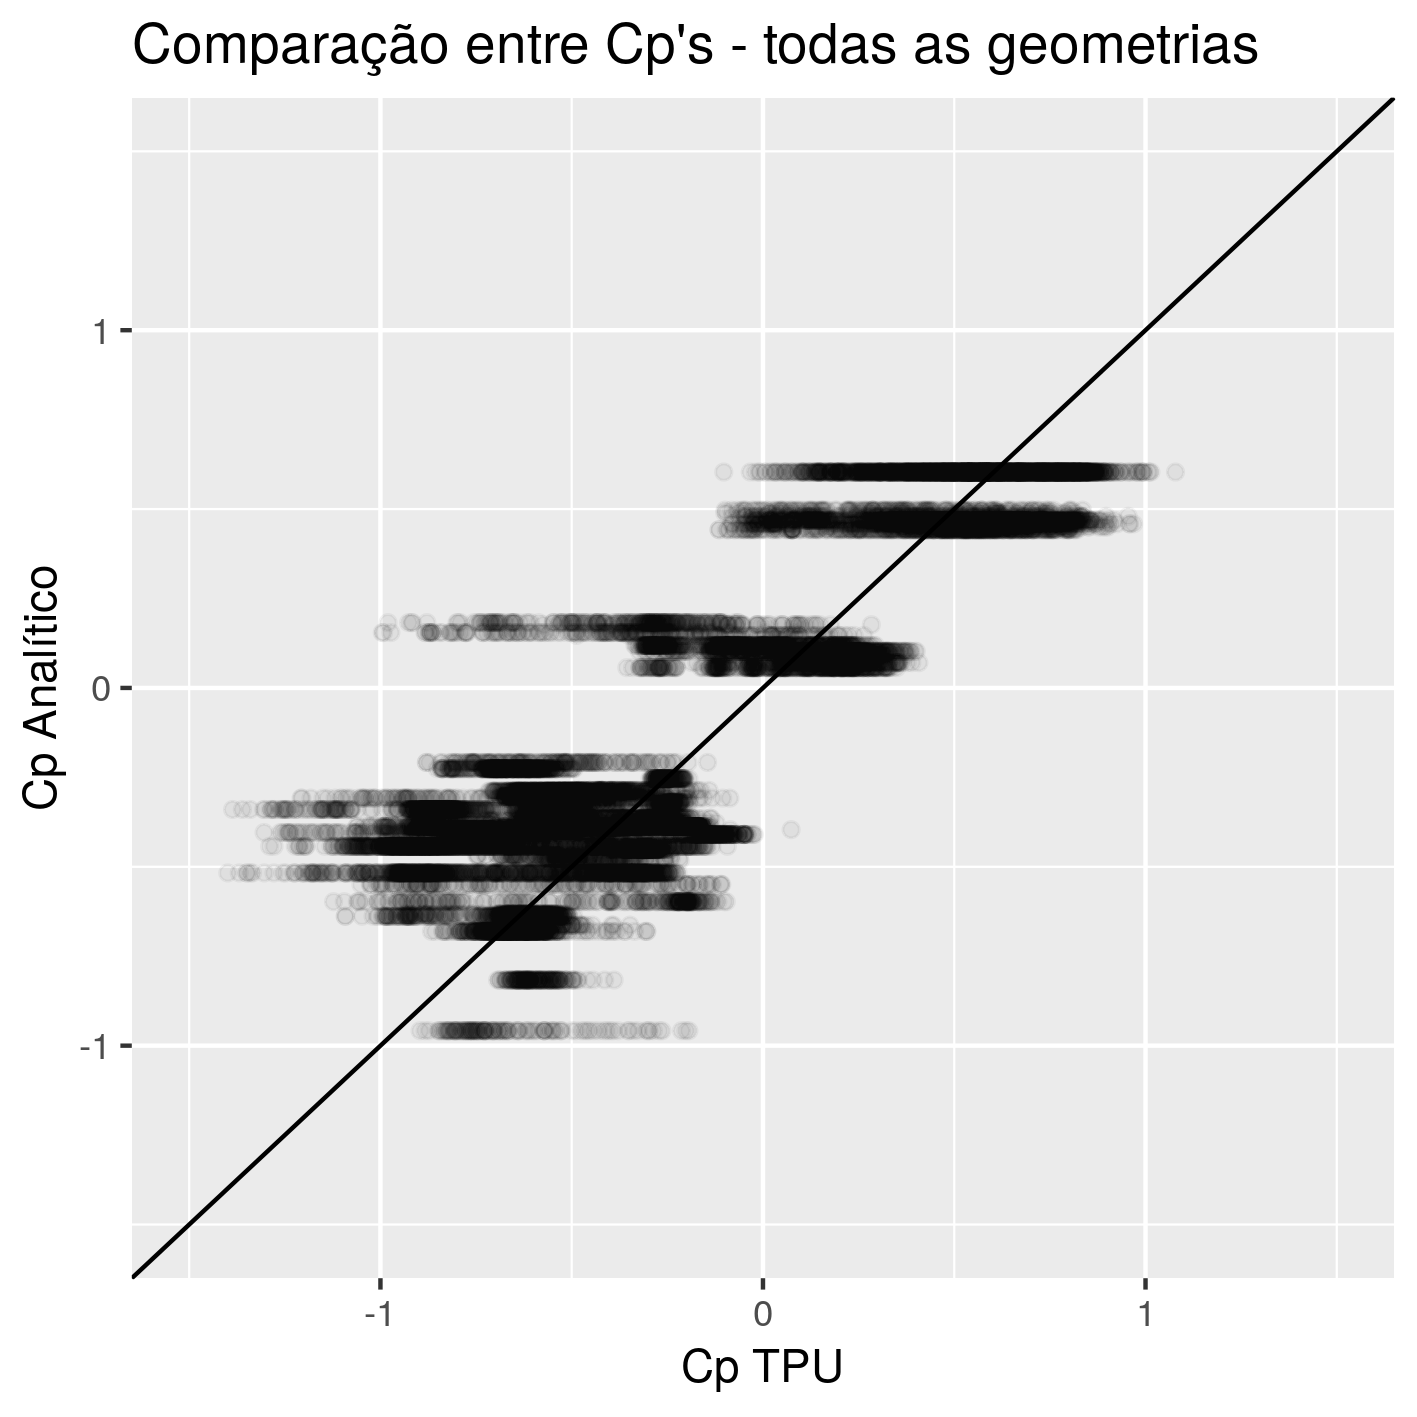
\includegraphics[width=1\linewidth]{img/cp_diff_scatter_all.png}
	\label{fig:cp_diff_scatter_all}
	%			\begin{flushleft}
	%				Fonte: o autor.
	%			\end{flushleft}
\end{figure}

Dentre as geometrias analisadas, a proporção com a maior diferença absoluta média entre os valores dos Cp’s foi igual a 0,344, para a geometria da edificação \textit{highrise} com proporções de largura, profundidade e altura igual a 2:1:2 (Figura \ref{fig:cp_diff_scatter}).

\begin{figure}[H]
	\centering
	\caption{Comparação entre os valores de Cp da geometria de proporções 2:1:2}
	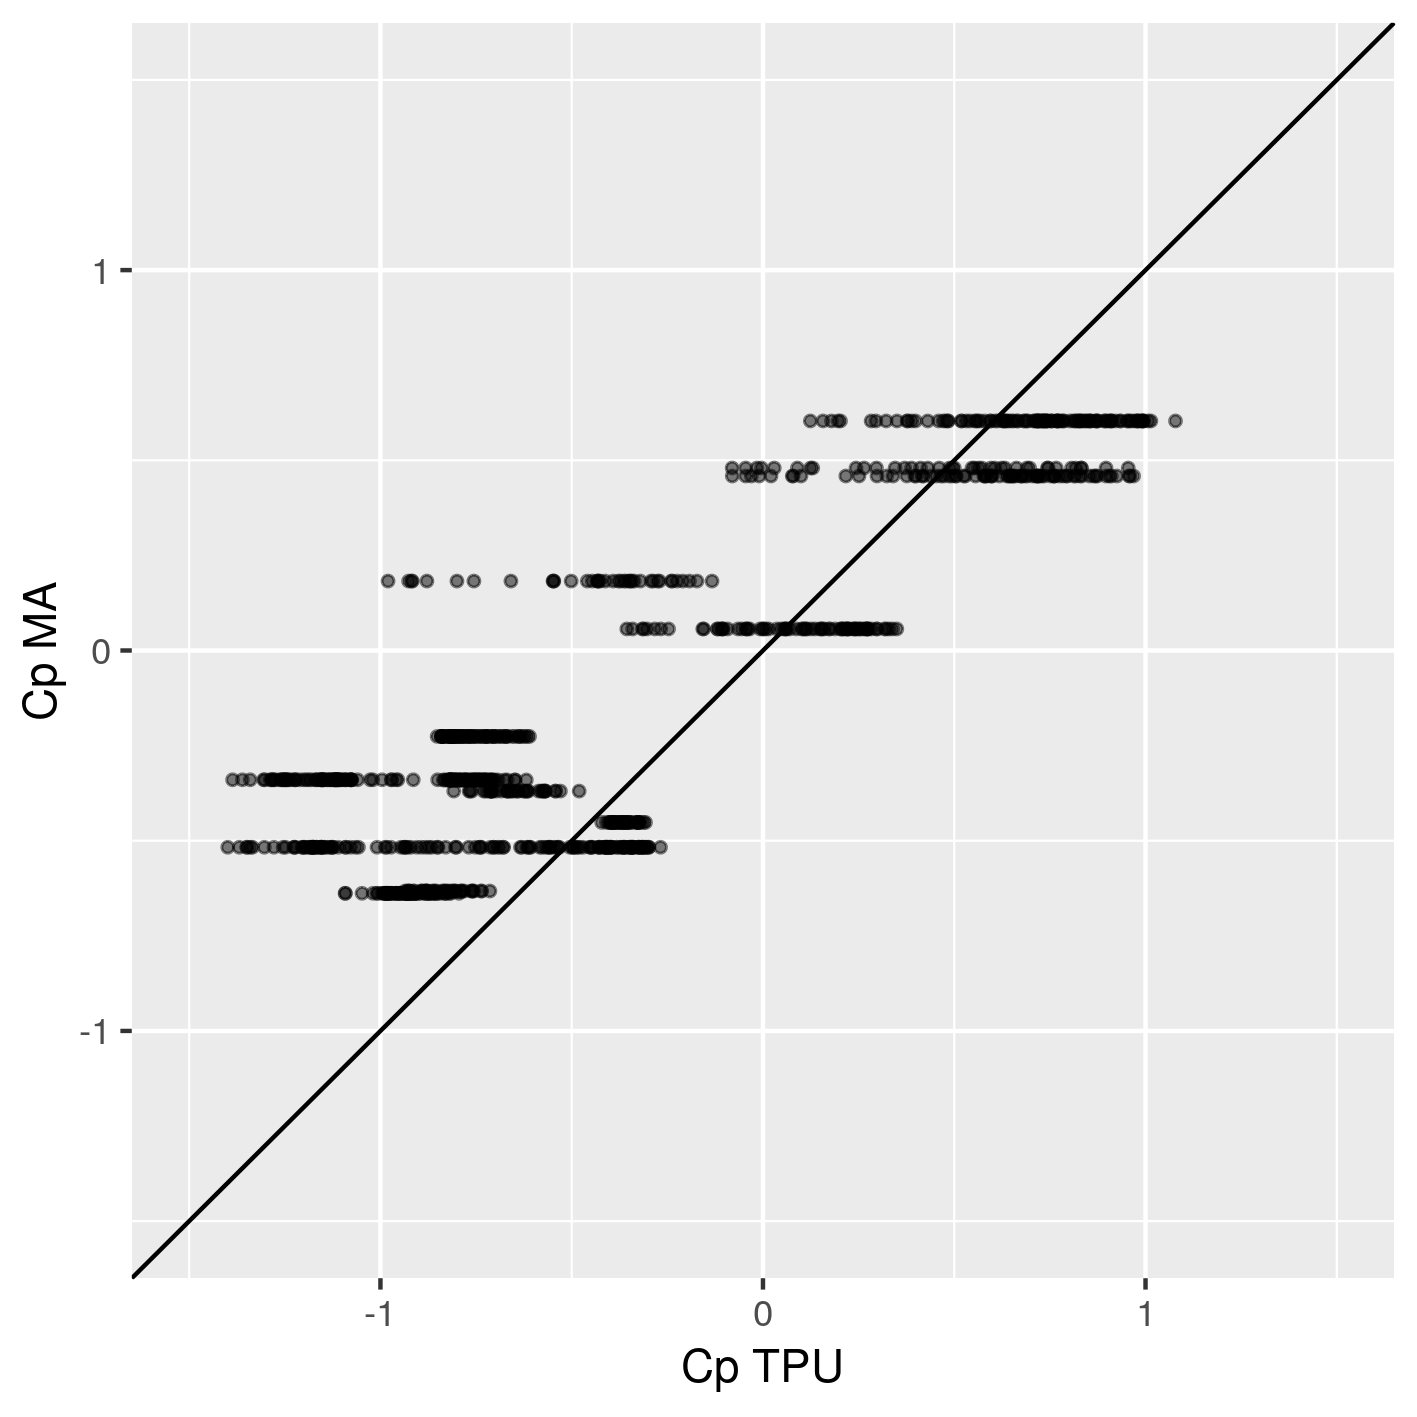
\includegraphics[width=1\linewidth]{img/cp_diff_scatter.png}
	\label{fig:cp_diff_scatter}
	%			\begin{flushleft}
	%				Fonte: o autor.
	%			\end{flushleft}
\end{figure}

A partir da comparação conduzida, decidiu-se comparar as diferenças nos resultados de simulações termoenergéticas utilizando como base uma tipologia com proporções de largura, profundidade e altura igual a 2:1:2.

Os resultados das 1000 simulações foram comparados por gráficos de pontos.
A comparação entre as médias anuais de trocas de ar por hora (ACH), apresentada na Figura \ref{fig:cpaverage_ACH_scatter}, mostra que o MA faz com que as simulações subestimem as trocas de ar nas simulações, possivelmente devido aos menores valores dos Cp's obtidos pelo método.
A diferença média foi igual a -0,67 para o ACH, com o erro absoluto do 95º percentil (AE95) é igual a 5,23 ACH.

\begin{figure}[H]
	\centering
	\caption{Comparação entre as médias anuais do ACH}
	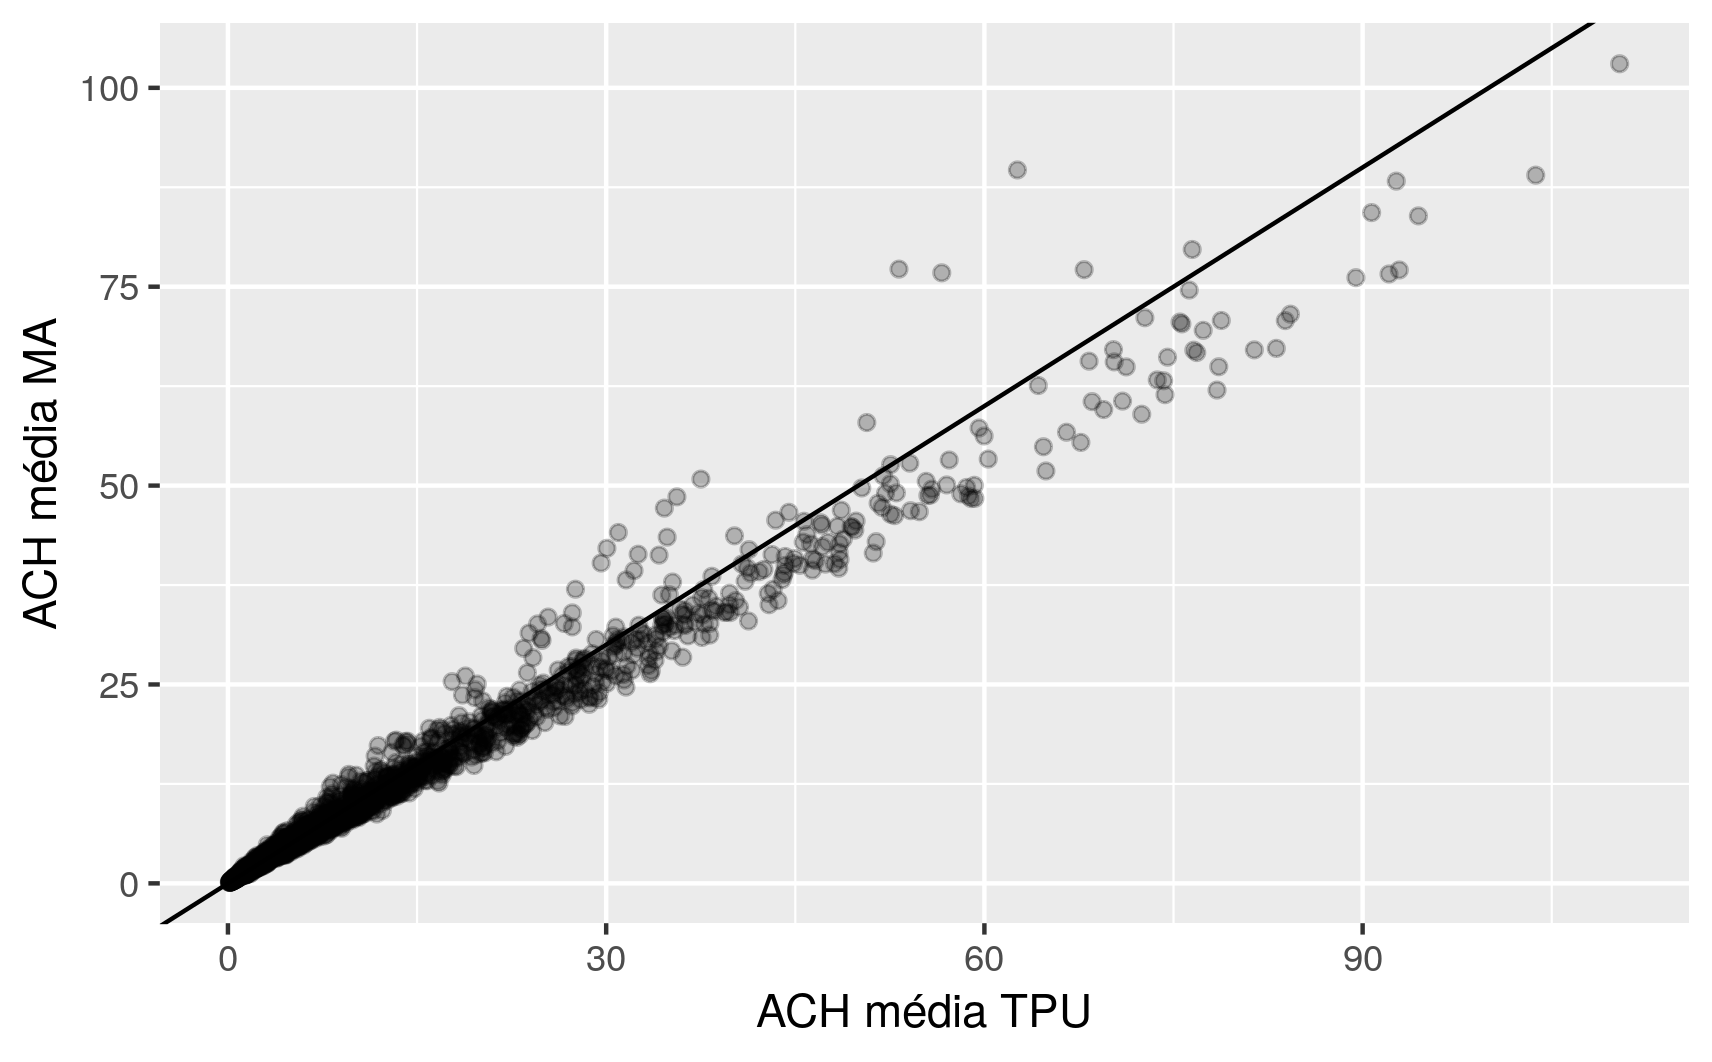
\includegraphics[width=1\linewidth]{img/cpaverage_ACH_scatter.png}
	\label{fig:cpaverage_ACH_scatter}
	%			\begin{flushleft}
	%				Fonte: o autor.
	%			\end{flushleft}
\end{figure}

Apesar dessas diferenças nas trocas de ar, a comparação entre as temperaturas operativas médias, apresentada na Figura \ref{fig:cpaverage_temp_scatter}, mostra que a diferença média da temperatura operativa é 0,04 $^{\circ}$C, sendo que o AE95 é igual a 0,31 $^{\circ}$C.
Essas diferenças são confirmadas como pouco significativas ao se analisar a Figura \ref{fig:cpaverage_EHF_scatter}, com a comparação da fração de horas em desconforto (EHF). A média de diferença do EHF nos casos analisados foi igual a 0,0037, com o AE95 igual a 0,0277.
Por tanto, considerou-se que a utilização do MA para calcular os valores dos Cp's é uma alternativa adequada para a simplificação das simulações termoenergéticas.

\begin{figure}[H]
	\centering
	\caption{Comparação entre as médias das temperaturas operativas}
	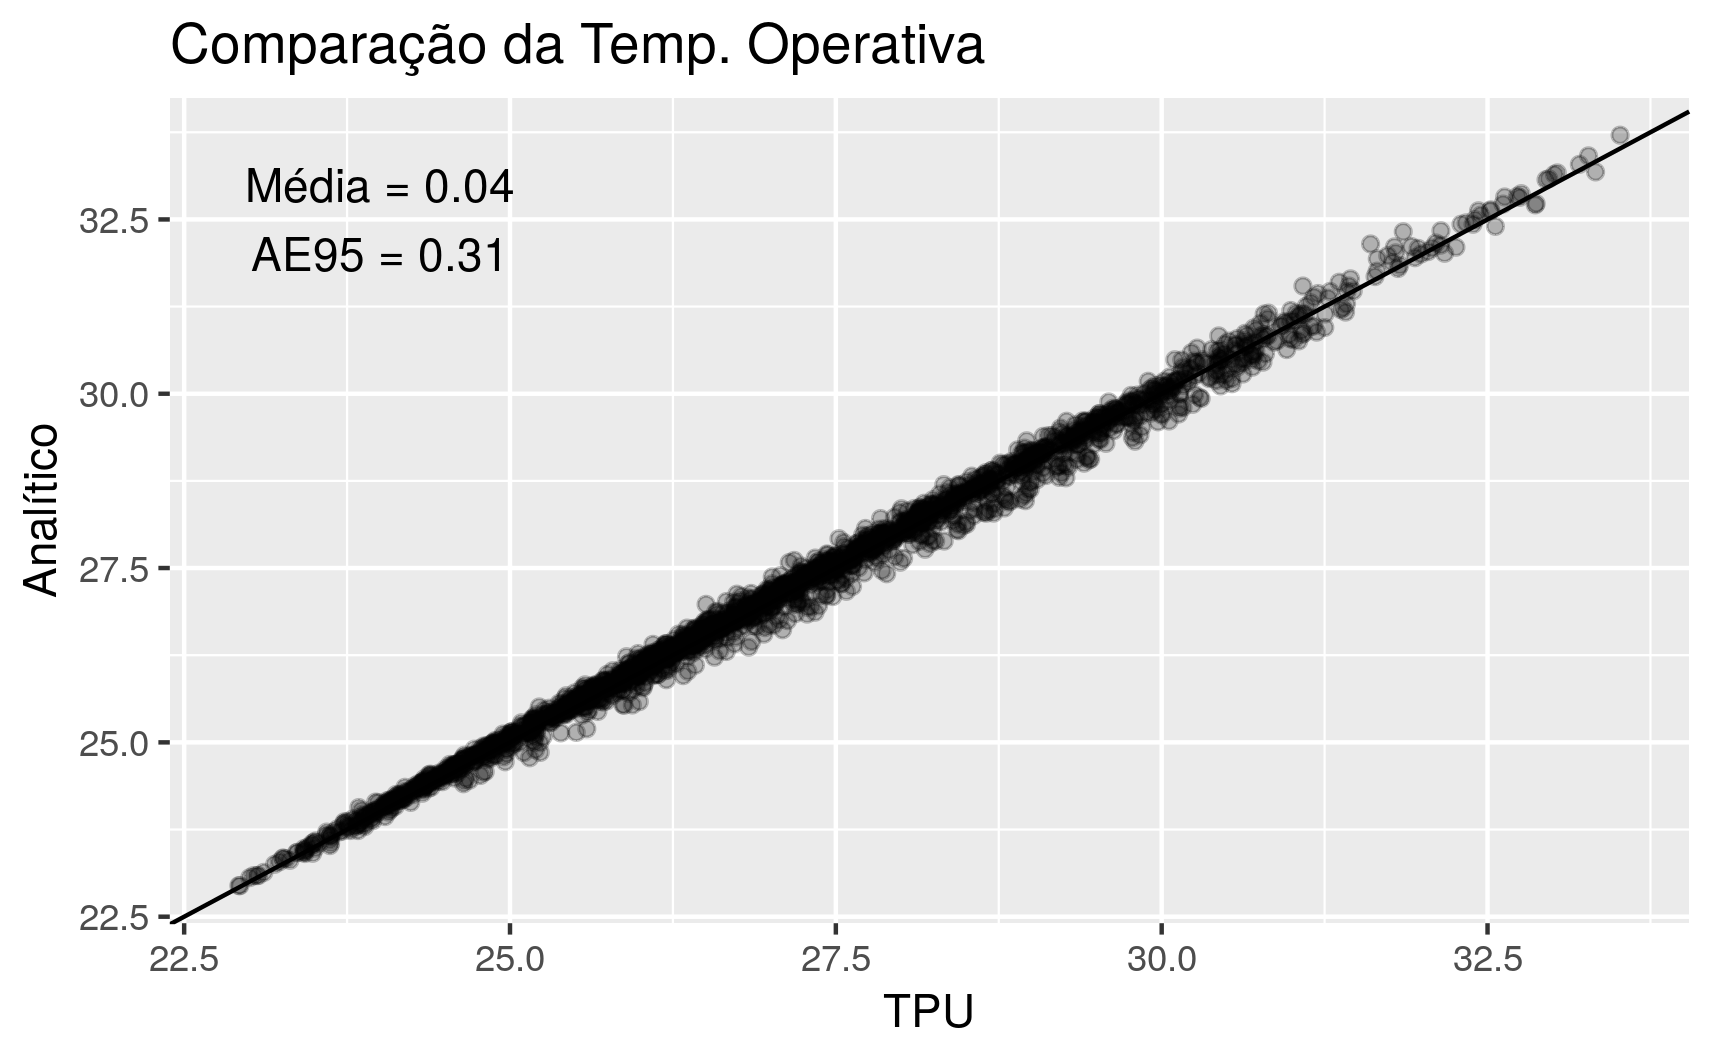
\includegraphics[width=1\linewidth]{img/cpaverage_temp_scatter.png}
	\label{fig:cpaverage_temp_scatter}
	%			\begin{flushleft}
	%				Fonte: o autor.
	%			\end{flushleft}
\end{figure}

\begin{figure}[H]
	\centering
	\caption{Comparação entre os resultados de EHF}
	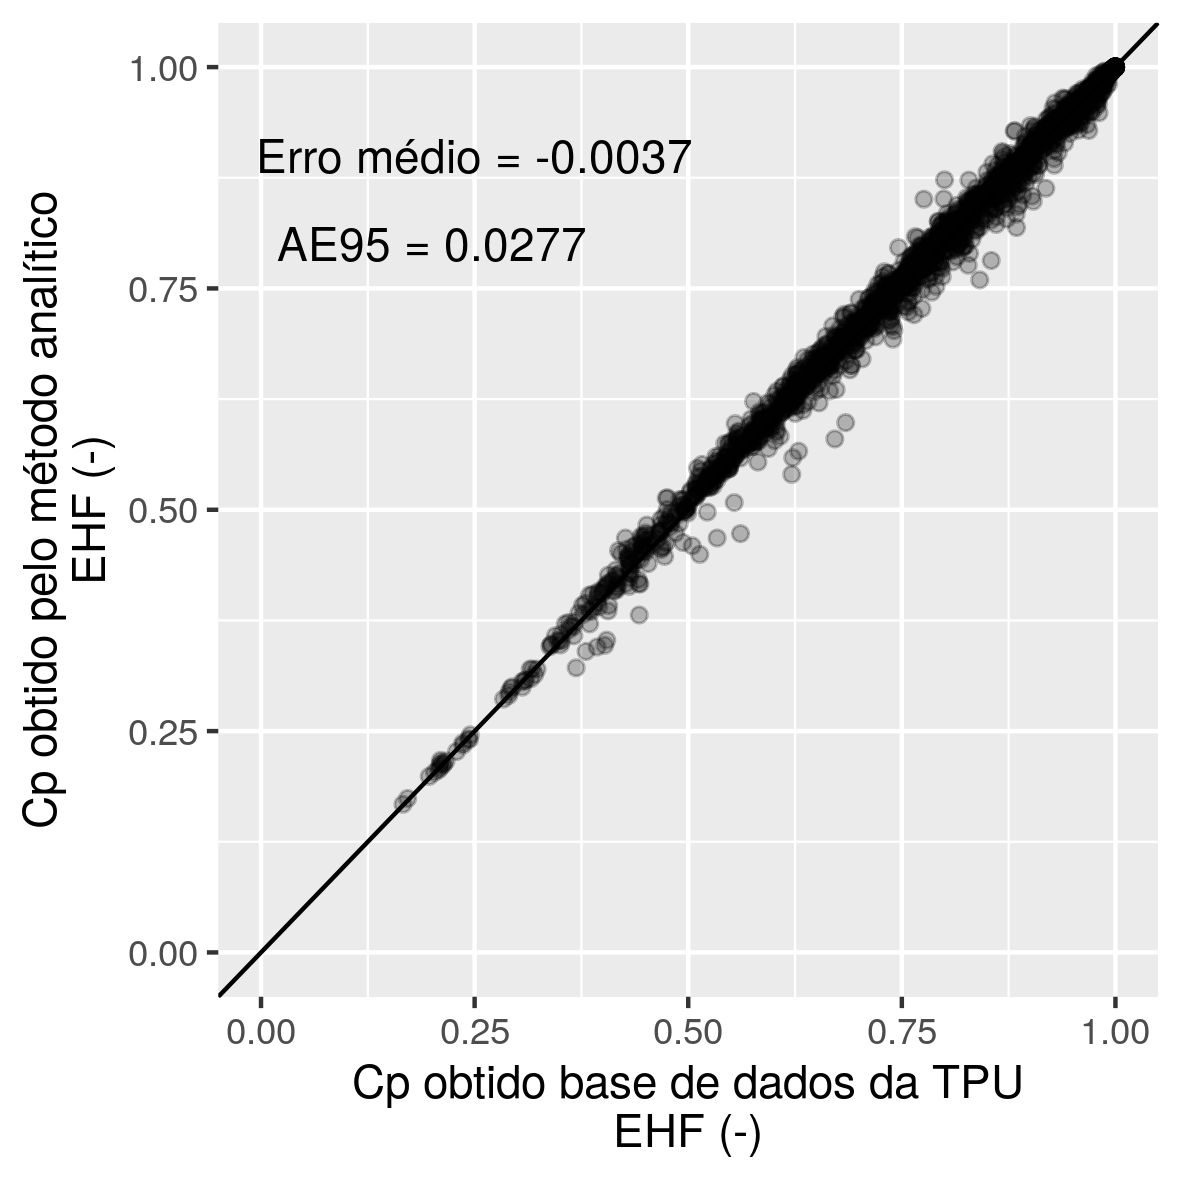
\includegraphics[width=1\linewidth]{img/cpaverage_EHF_scatter.png}
	\label{fig:cpaverage_EHF_scatter}
	%			\begin{flushleft}
	%				Fonte: o autor.
	%			\end{flushleft}
\end{figure}

\subsection{Representação da envoltória com duas camadas}

Os resultados das simulações com as paredes equivalentes subestimaram o EHF em 0,0107 na média, quando comparados aos resultados das simulações com as paredes de referência. 
Os resultados das simulações para a parede de gesso com isolamento resultaram em um erro absolto médio igual a 0,0100, e um AE95 igual a 0,0604 para o EHF (Figura \ref{fig:par3_scatter}).

\begin{figure}[H]
	\centering
	\caption{Comparação entre os resultados de EHF para a parede de gesso com isolamento}
	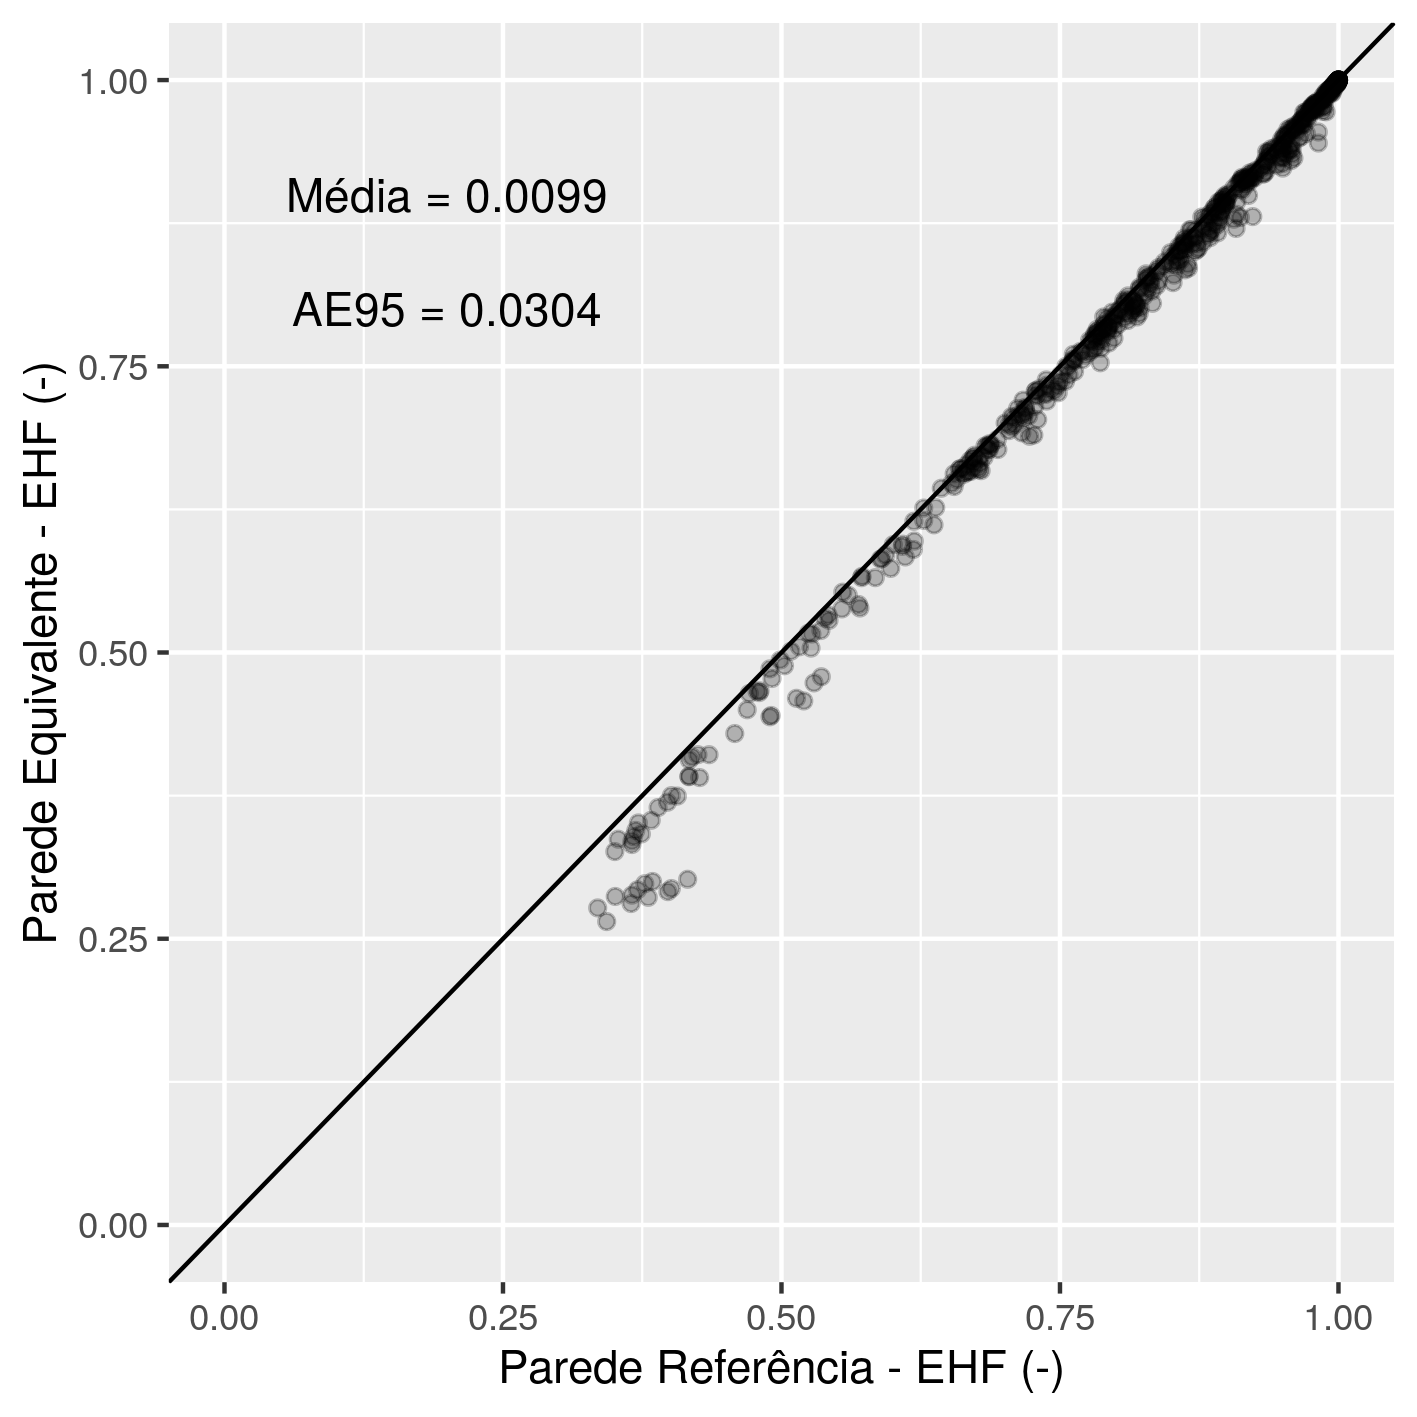
\includegraphics[width=1\linewidth]{img/paredeeq_EHF_par3_scatter.png}
	\label{fig:par3_scatter}
	%			\begin{flushleft}
	%				Fonte: o autor.
	%			\end{flushleft}
\end{figure}

A representação da parede de alvenaria apresenta-se mais adequada considerando-se apenas metade da parede para definir a capacidade térmica. Enquanto que, para a parede com a capacidade térmica total o erro absoluto médio foi igual a 0,0209, e o AE95 foi igual a 0,0650, para a parede de alvenaria com metade da capacidade térmica considerada, o erro médio absoluto foi igual a 0,0189, e o AE95 foi igual a 0,0604.

\begin{figure}[H]
	\centering
	\caption{Comparação entre os resultados de EHF para a parede de alvenaria com capacidade térmica total}
	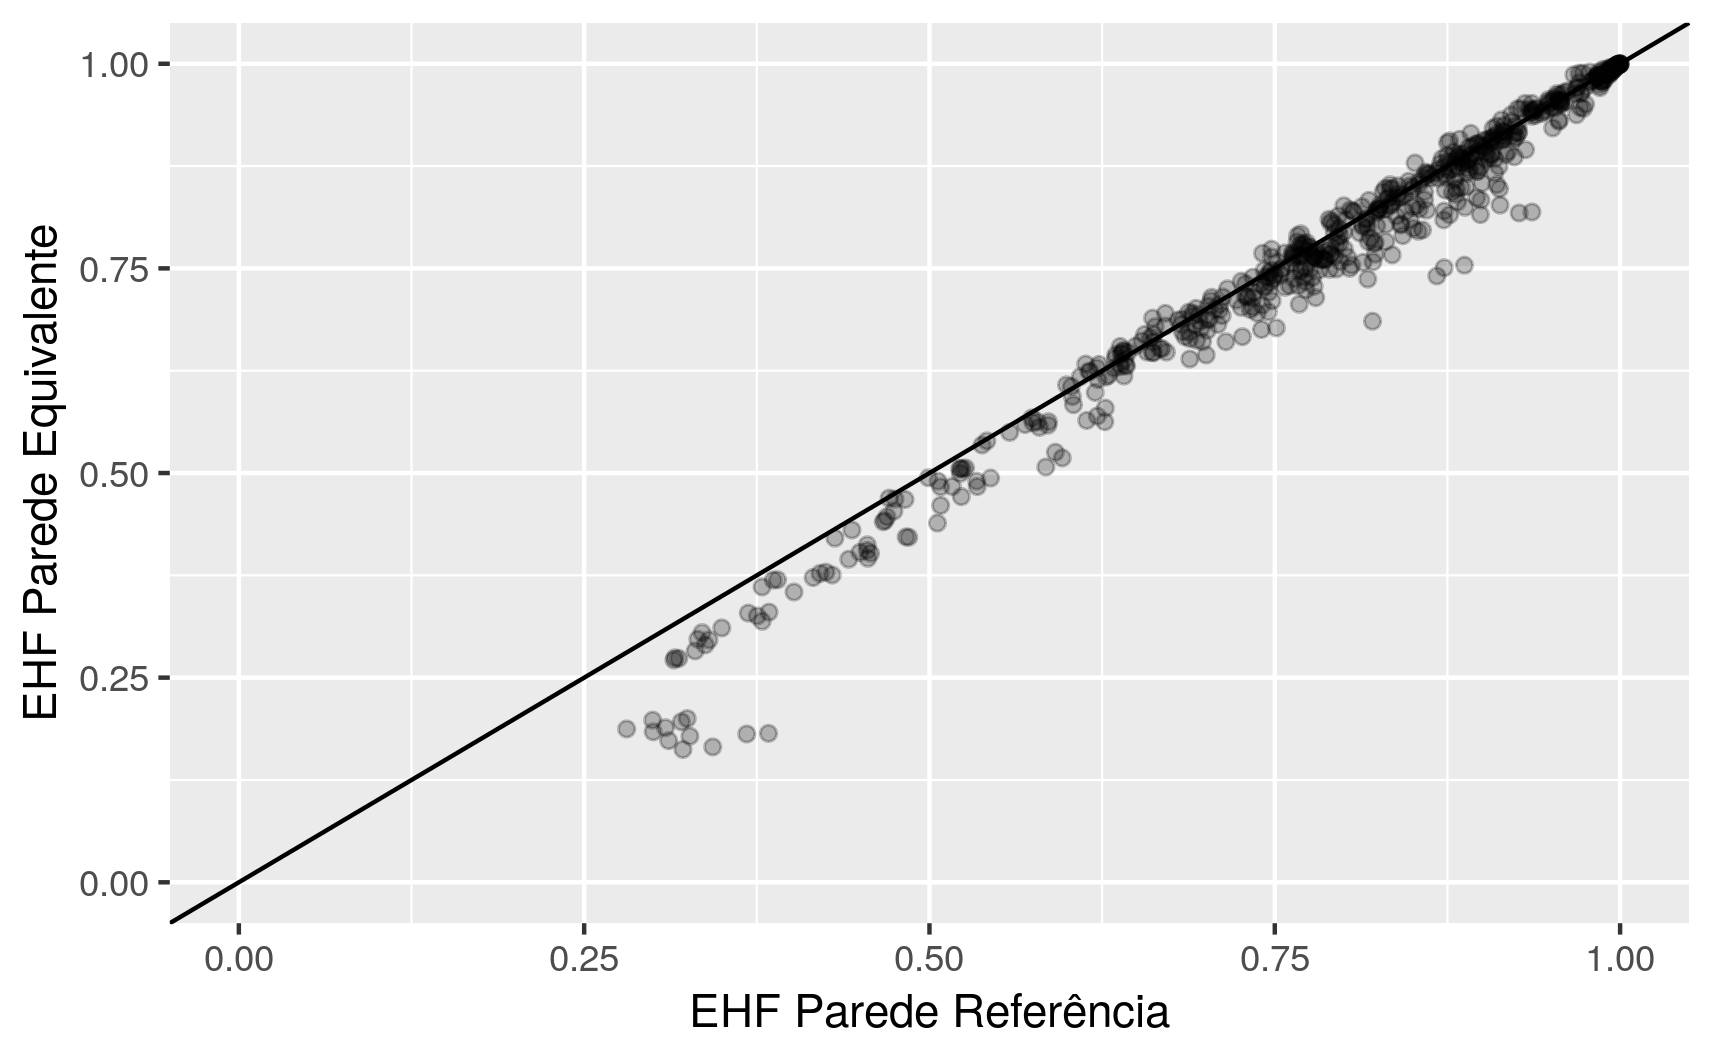
\includegraphics[width=1\linewidth]{img/paredeeq_EHF_par2a_scatter.png}
	\label{fig:par2a_scatter}
	%			\begin{flushleft}
	%				Fonte: o autor.
	%			\end{flushleft}
\end{figure}
\begin{figure}[H]
	\centering
	\caption{Comparação entre os resultados de EHF para a parede de alvenaria com metade da capacidade térmica}
	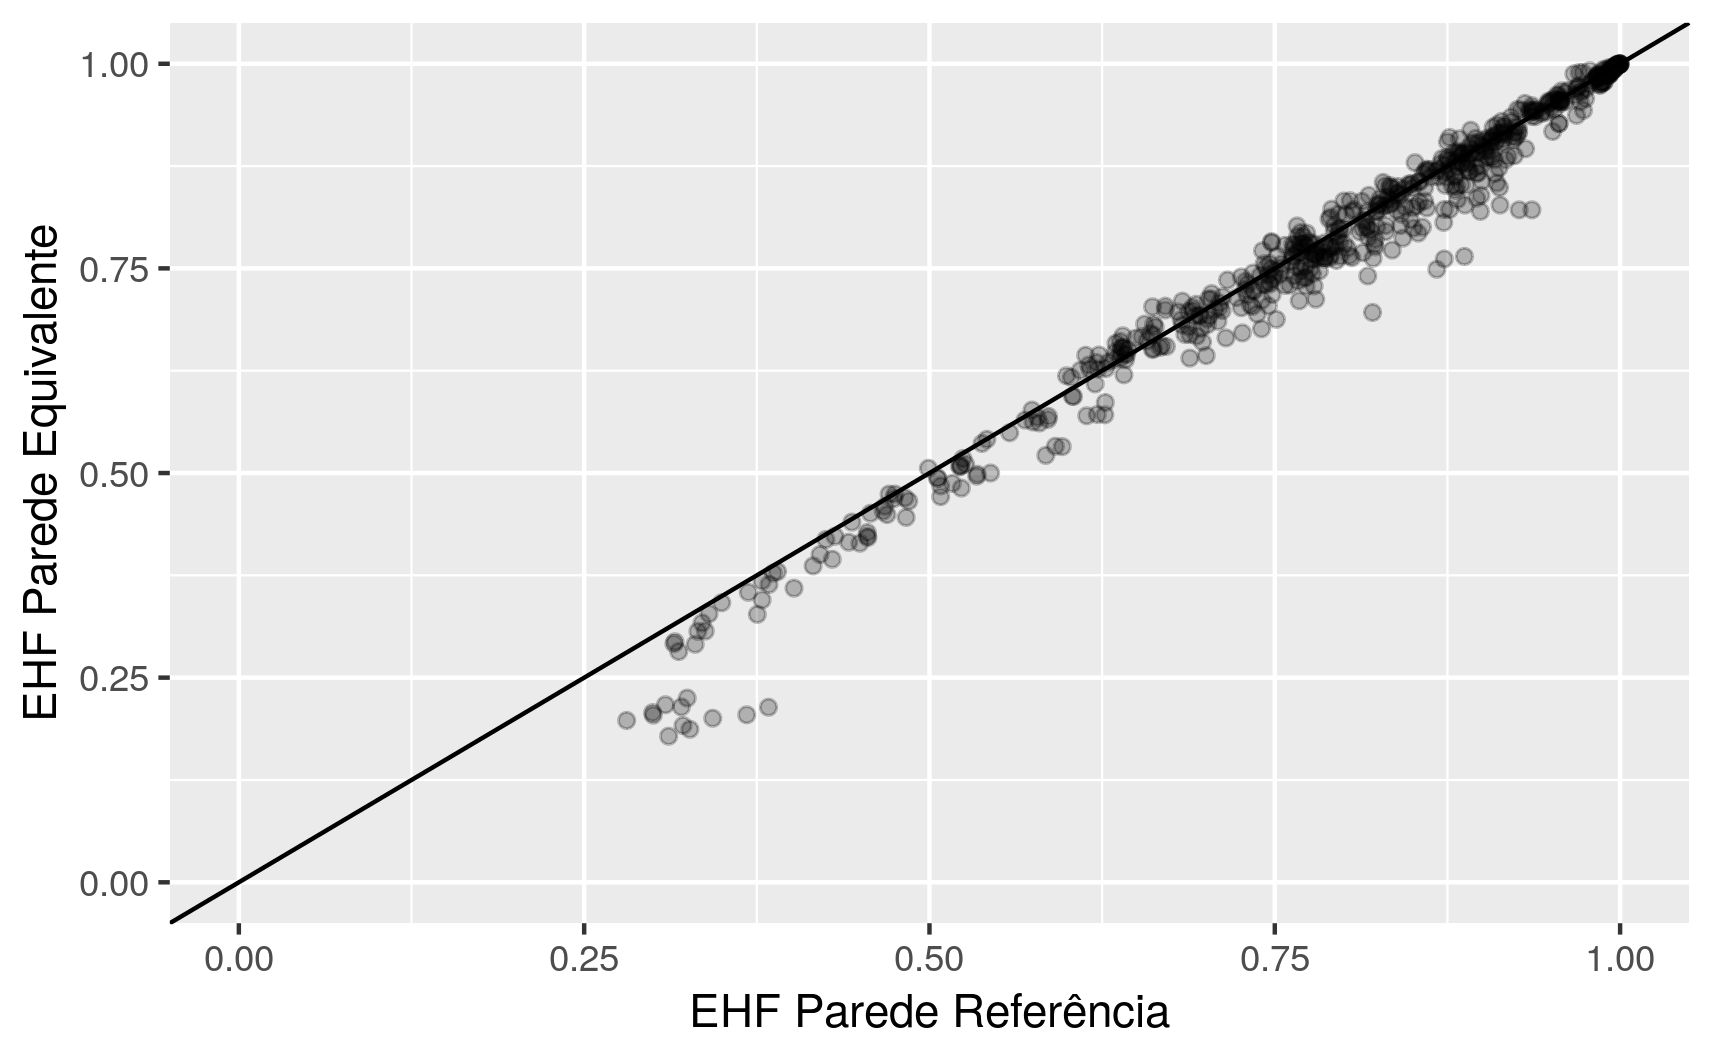
\includegraphics[width=1\linewidth]{img/paredeeq_EHF_par2b_scatter.png}
	\label{fig:par2b_scatter}
	%			\begin{flushleft}
	%				Fonte: o autor.
	%			\end{flushleft}
\end{figure}

O caso com as maiores diferenças no EHF foi para uma edificação em contato com o solo, com cobertura exposta, e um fator de abertura da janela igual a 0,23.
Apesar das diferenças nos resultados, o uso da parede equivalente facilita a parametrização da transmitância térmica e da capacidade térmica. Por esse motivo, considerou-se as diferenças pouco significativas, e a parede equivalente foi adotada para simplificar as simulações.

\subsection{Condição de contorno das paredes adjacentes à edificação}

A simplificação das simulações adotando-se apenas uma zona térmica foi avaliada para duas condições de contorno. Os resultados mostram que a maneira mais adequada de representar as paredes adjacentes à circulação da edificação é considerando-as como adiabáticas. Considerar as paredes adjacentes à circulação como \textit{Outdoors}, faz com que os resultados do EHF sejam subestimados em 0,0868 em média, como AE95 igual a 0,1865 (Figura \ref{fig:szout_EHF}).

\begin{figure}[H]
	\centering
	\caption{Comparação entre os resultados de EHF para parede \textit{Outdoors}}
	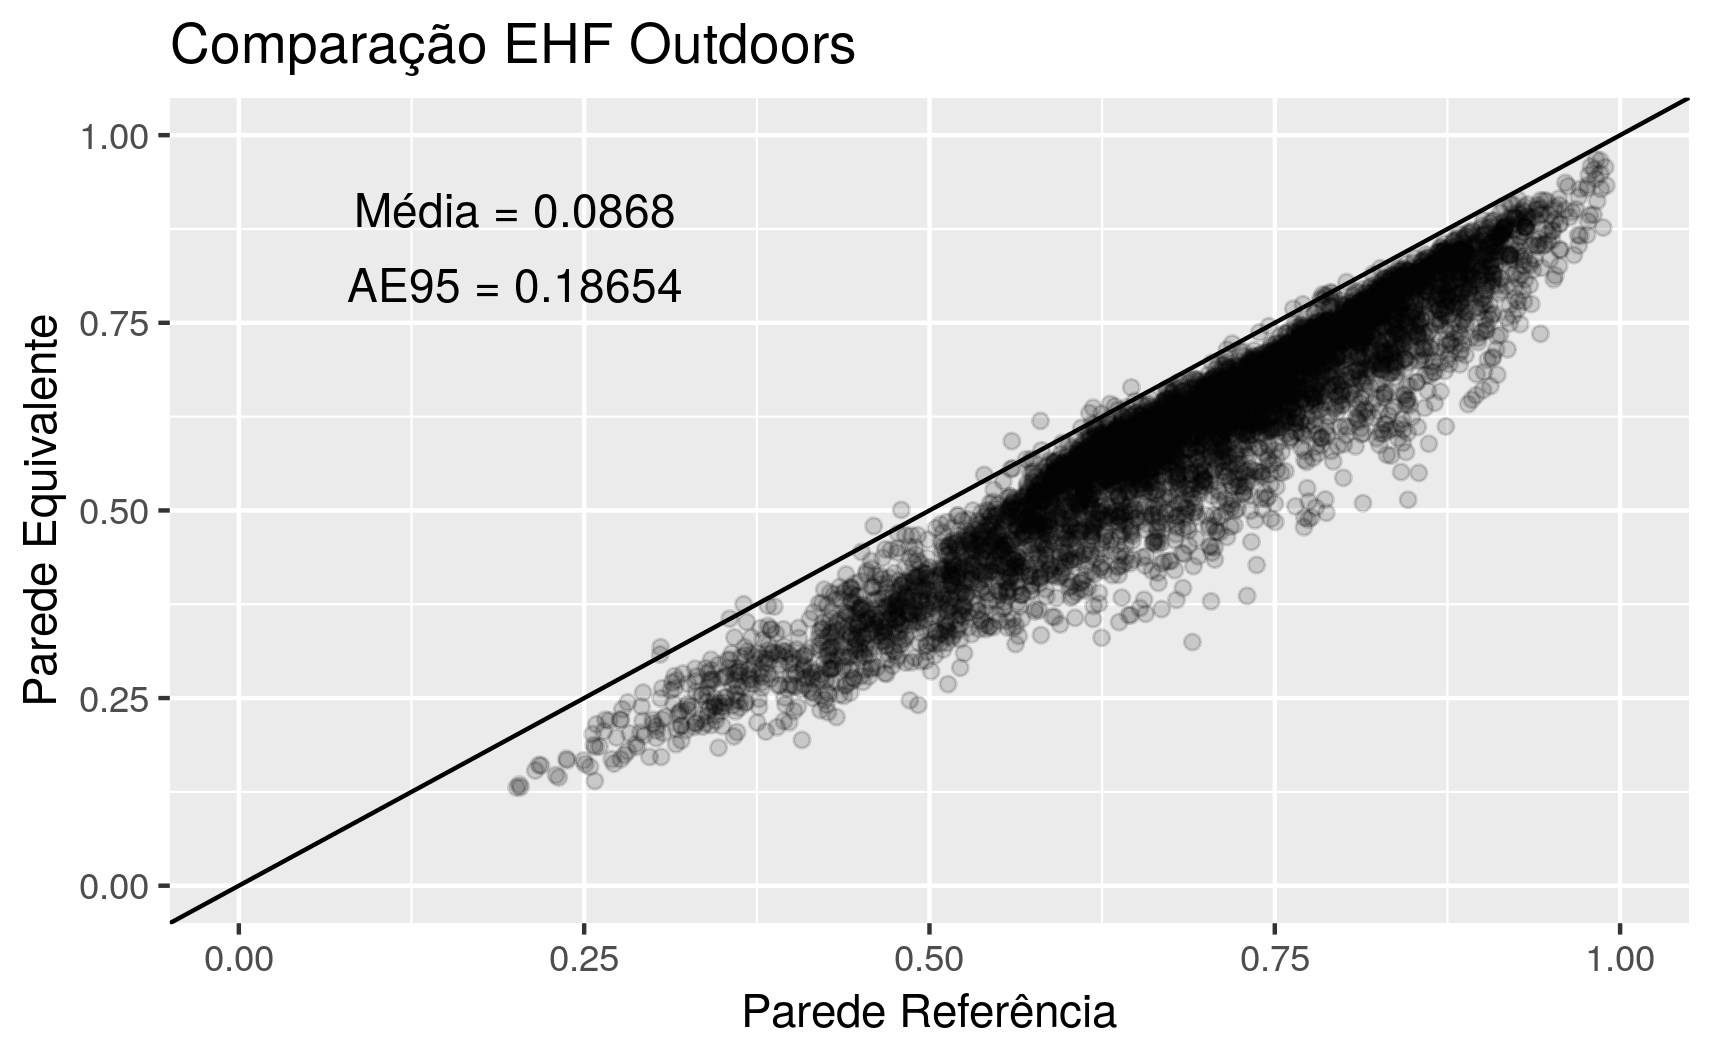
\includegraphics[width=1\linewidth]{img/szout_EHF_scatter.png}
	\label{fig:szout_EHF}
	%			\begin{flushleft}
	%				Fonte: o autor.
	%			\end{flushleft}
\end{figure}

Os resultados das simulações considerando-se as paredes voltadas para o corredor como adiabáticas subestimaram o EHF em 0,0051 na média, como AE95 igual a 0,0804 (Figura \ref{fig:szadi_EHF}).

\begin{figure}[H]
	\centering
	\caption{Comparação entre os resultados de EHF para parede adiabática}
	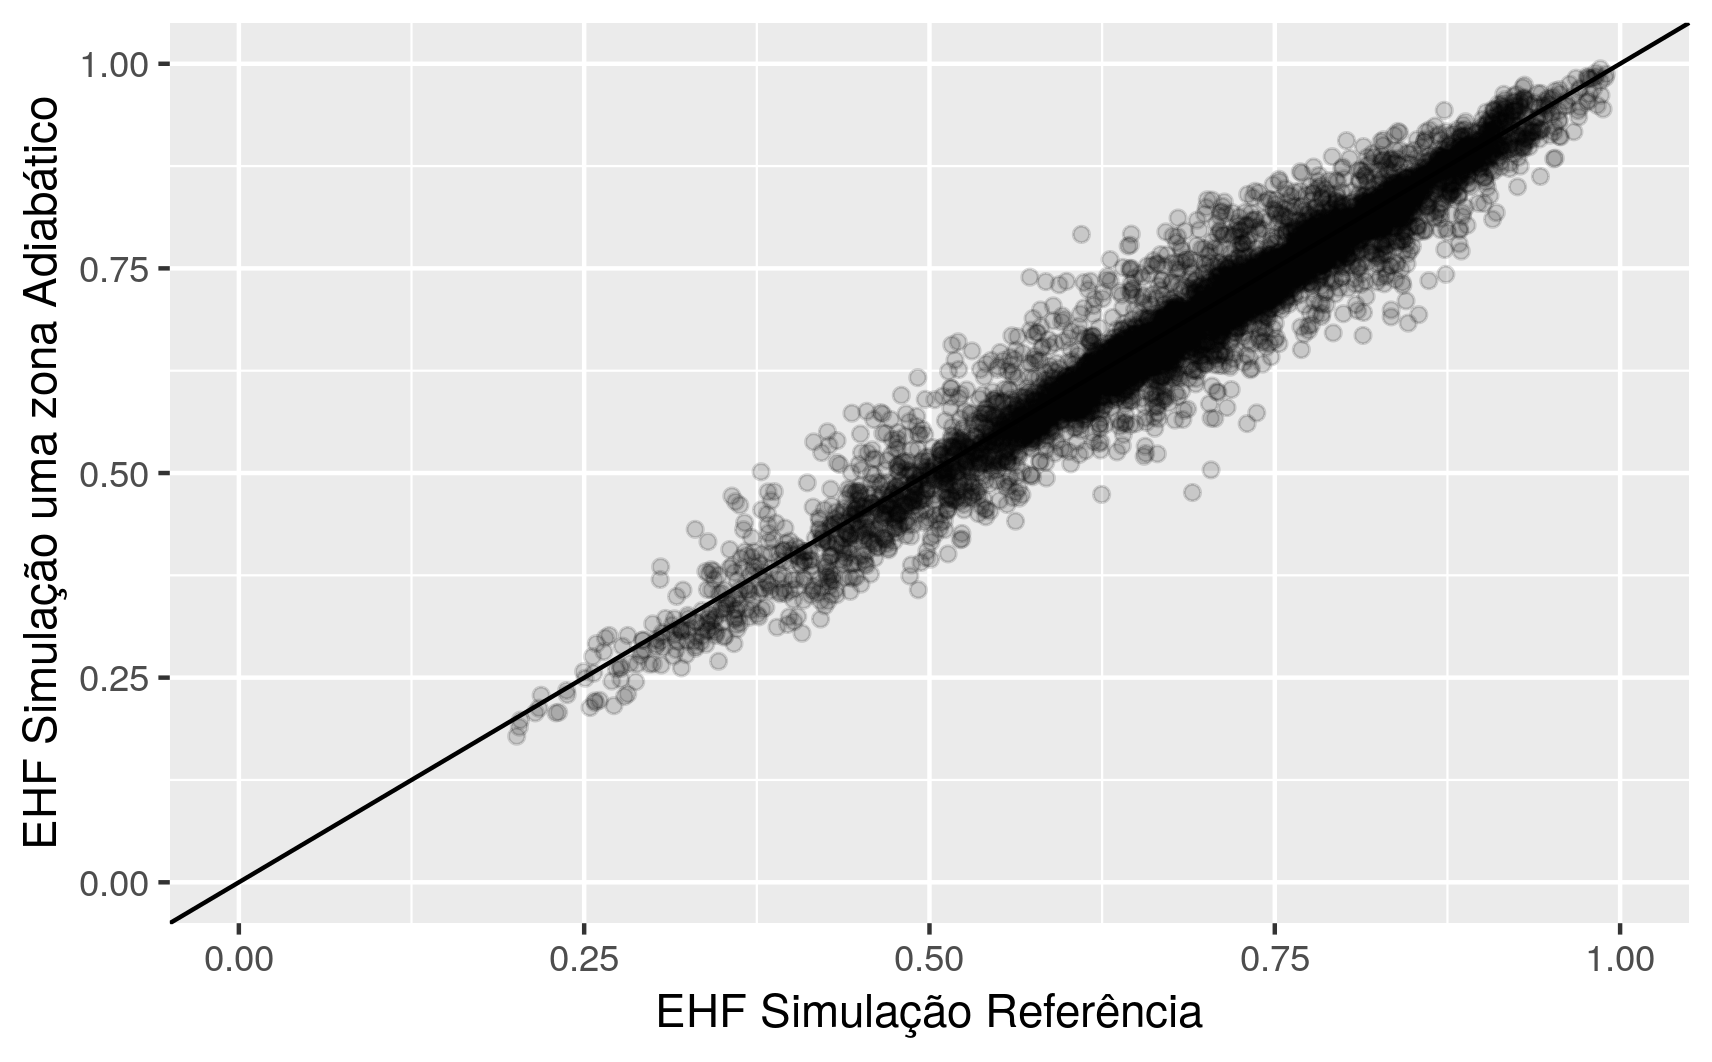
\includegraphics[width=1\linewidth]{img/szadi_EHF_scatter.png}
	\label{fig:szadi_EHF}
	%			\begin{flushleft}
	%				Fonte: o autor.
	%			\end{flushleft}
\end{figure}

A partir dos resultados obtidos, definiu-se as paredes voltadas para a circulação como adiabáticas no desenvolvimento das simulações simplificadas.

\subsection{Modelagem da ventilação natural na simulação simplificada}

Nesta etapa do trabalho as simulações foram conduzidas para se obter duas respostas:
(1) se é adequado o uso do coeficiente de pressão equivalente ($Cp_{eq}$) para ser associado à porta da zona térmica; (2) qual deveria ser o coeficiente de fluxo mássico de ar adotado para o objeto \textit{AirflowNetwork:MultiZone:Surface:Crack}.

Para analisar simultaneamente o desempenho do $Cp_{eq}$ e dos coeficientes de fluxo mássico de ar, o gráfico da Figura \ref{fig:pareto} foi gerado, observando-se as raízes dos erros médios quadráticos (RMSE).
É possível observar que as simulações desenvolvidas utilizando-se o $Cp_{eq}$ obtiveram resultados com RMSE menores do que as simulações desenvolvidas utilizando-se o Cp obtido diretamente pelo MA.
Para a definir o coeficiente de fluxo mássico de ar, levou-se em conta inicialmente os erros relacionados ao ACH.
No entanto, foi identificada uma fronteira de Pareto entre os erros analisados, que mostra como a busca por menores erros de ACH aumenta os erros relacionados ao EHF.
O resultado dessa análise levanta duas suspeitas. A primeira é de que as diferenças maiores nas trocas de ar anulem erros relacionados à definição das paredes adjacentes à edificação como adiabáticas. A segunda hipótese, é de que os maiores erros relacionados ao MACH sejam em casos onde as diferenças nas trocas de ar não sejam relevantes para alterar a temperatura operativa nas zonas térmicas e, consequentemente, o EHF.

\begin{figure}[H]
	\centering
	\caption{Eficiência de Pareto entre EHF e ACH médio}
	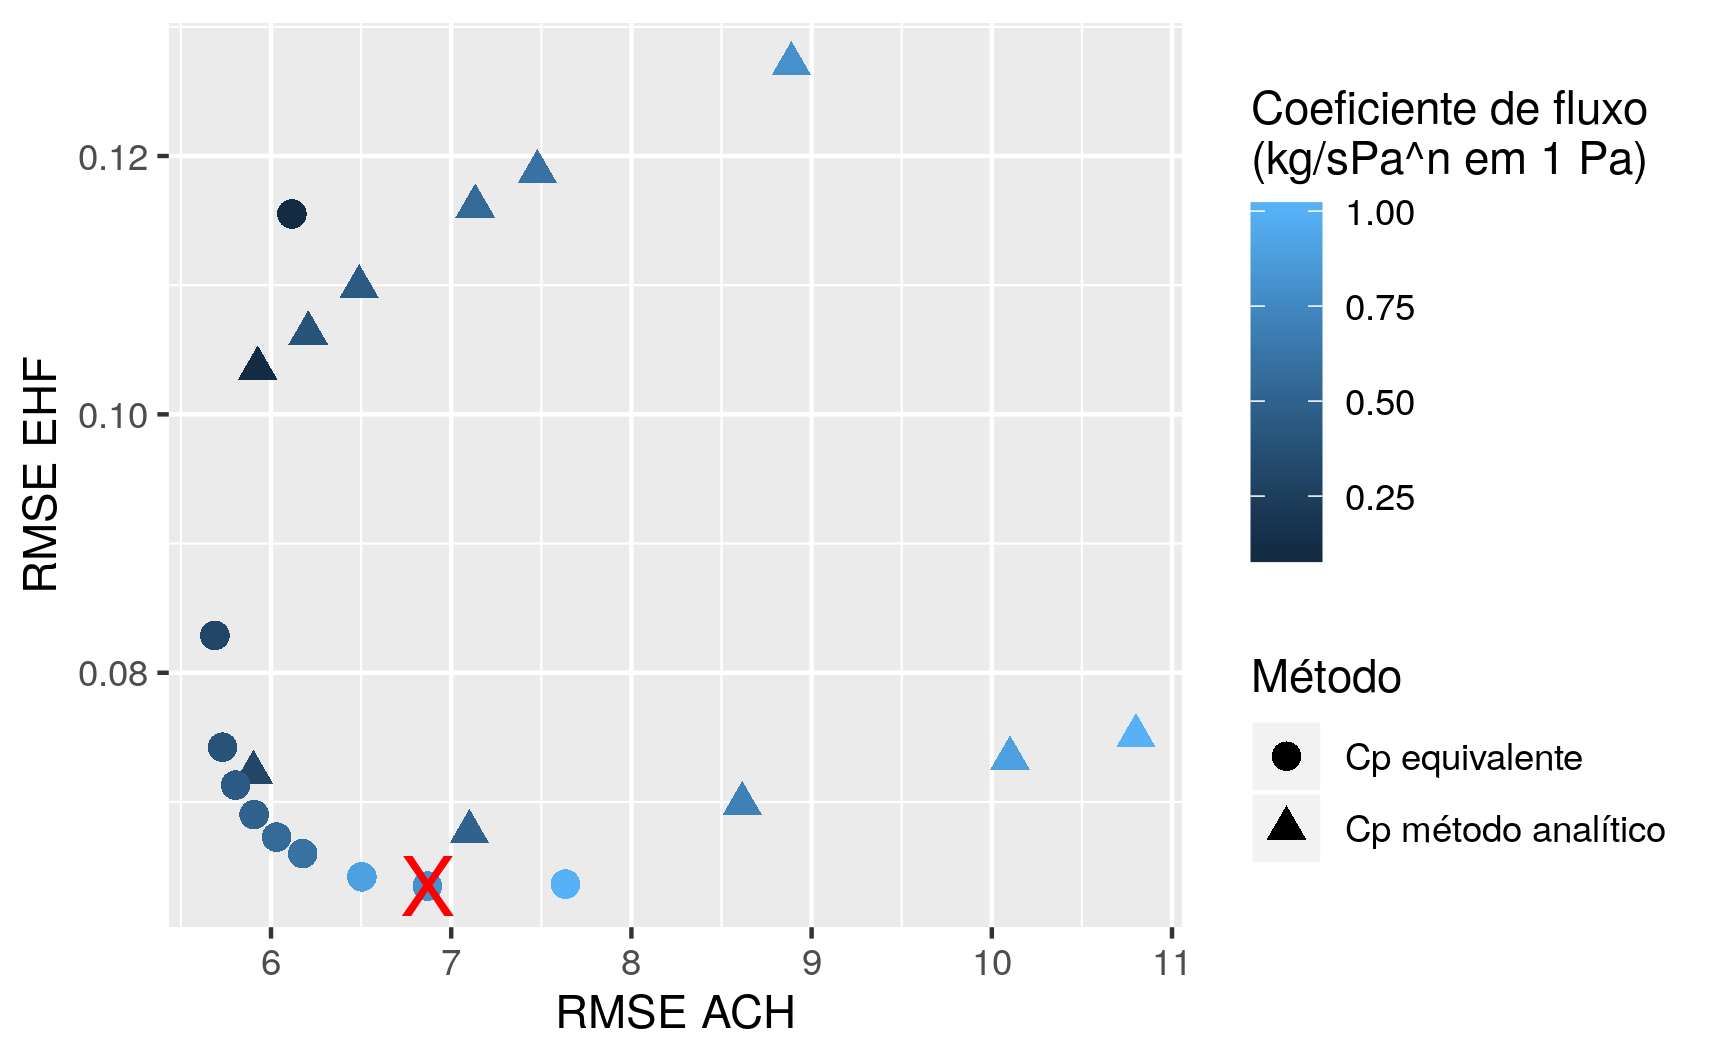
\includegraphics[width=1\linewidth]{img/cpeq_pareto.png}
	\label{fig:pareto}
	%			\begin{flushleft}
	%				Fonte: o autor.
	%			\end{flushleft}
\end{figure}

Como o desenvolvimento das simulações é voltado para obter a maior precisão possível para os resultados de EHF, optou-se por definir o coeficiente de fluxo mássico de ar com valor igual a 0,8, pois as simulações desenvolvidas utilizando-se este valor estão na fronteira de Pareto, e resultaram nos menores erros de EHF.

\subsection{Análise de sensibilidade}

As Figuras \ref{fig:as_ach}, \ref{fig:as_temp} e \ref{fig:as_ehf} apresentam os resultados das análises de sensibilidade (AS) para efeitos de primeira ordem e efeitos totais, relacionados ao ACH, às temperaturas operativas das zonas, e ao EHF. Os índices apresentados são proporcionais às influências entre os dados de entrada e saída.

\begin{figure}[H]
	\centering
	\caption{AS de Sobol dos efeitos de primeira ordem e efeitos totais nas médias anuais de ACH}
	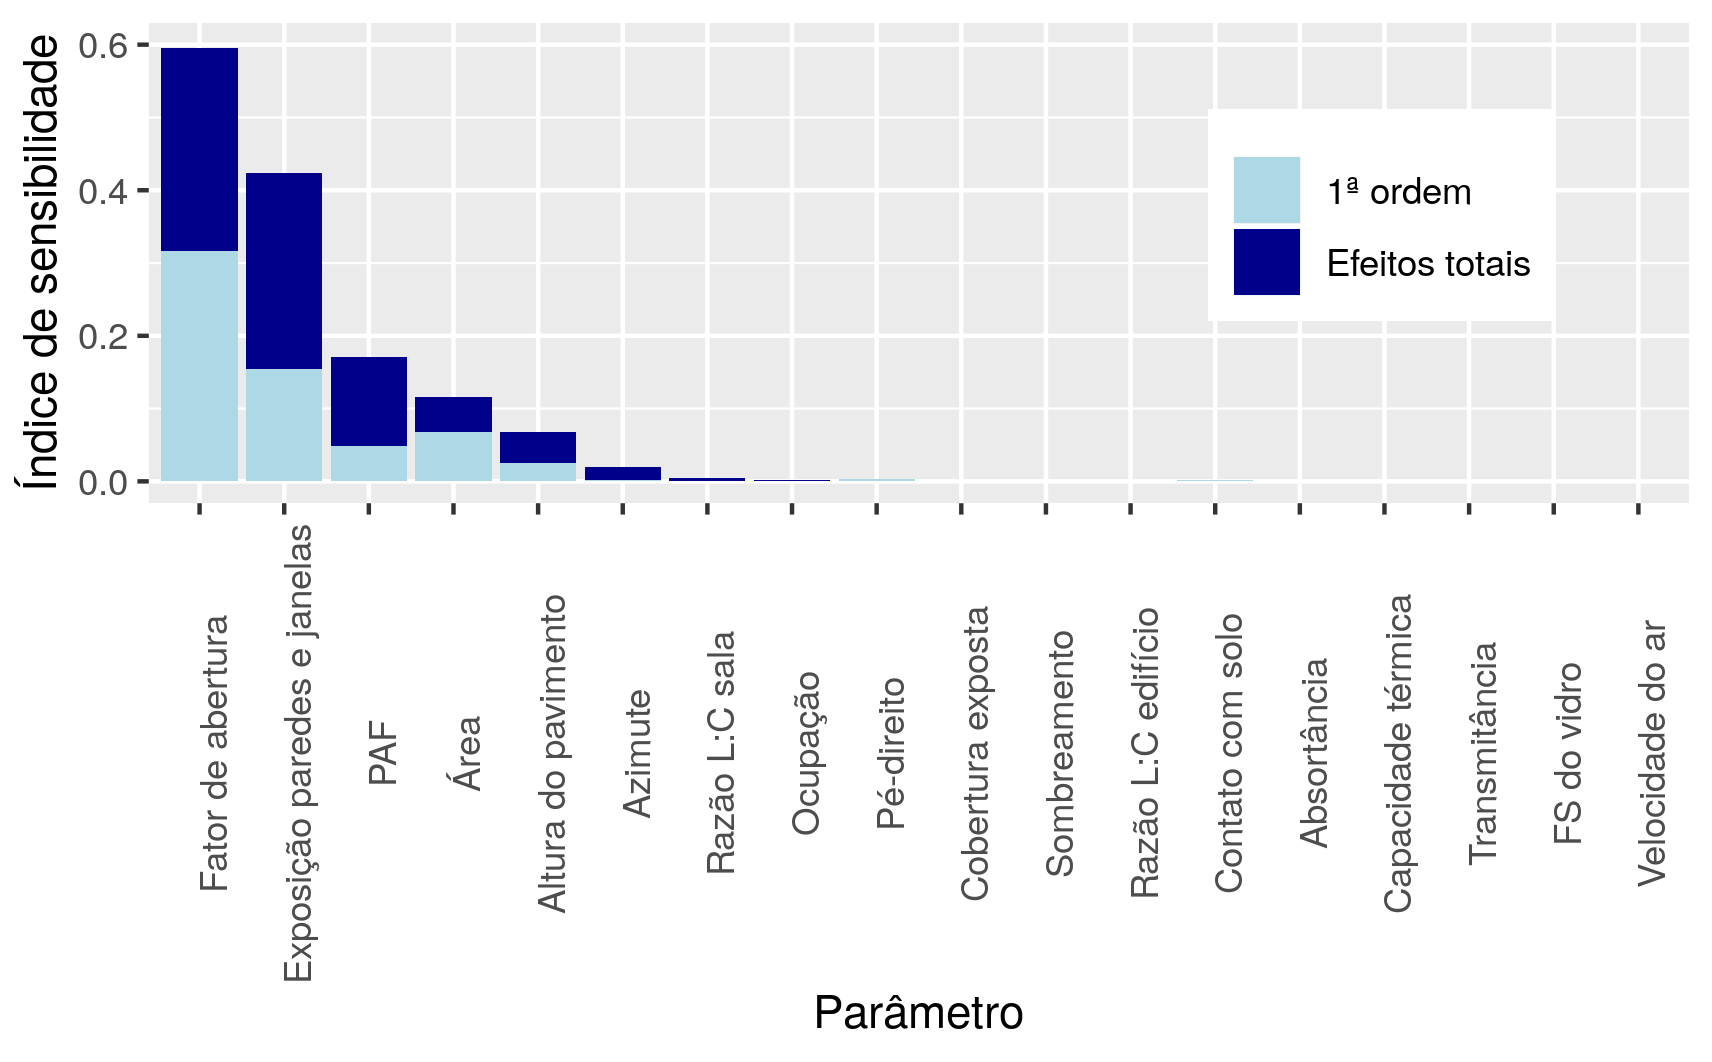
\includegraphics[width=1\linewidth]{img/as_ach.png}
	\label{fig:as_ach}
	%			\begin{flushleft}
	%				Fonte: o autor.
	%			\end{flushleft}
\end{figure}

\begin{figure}[H]
	\centering
	\caption{AS de Sobol dos efeitos de primeira ordem e efeitos totais nas temperaturas operativas}
	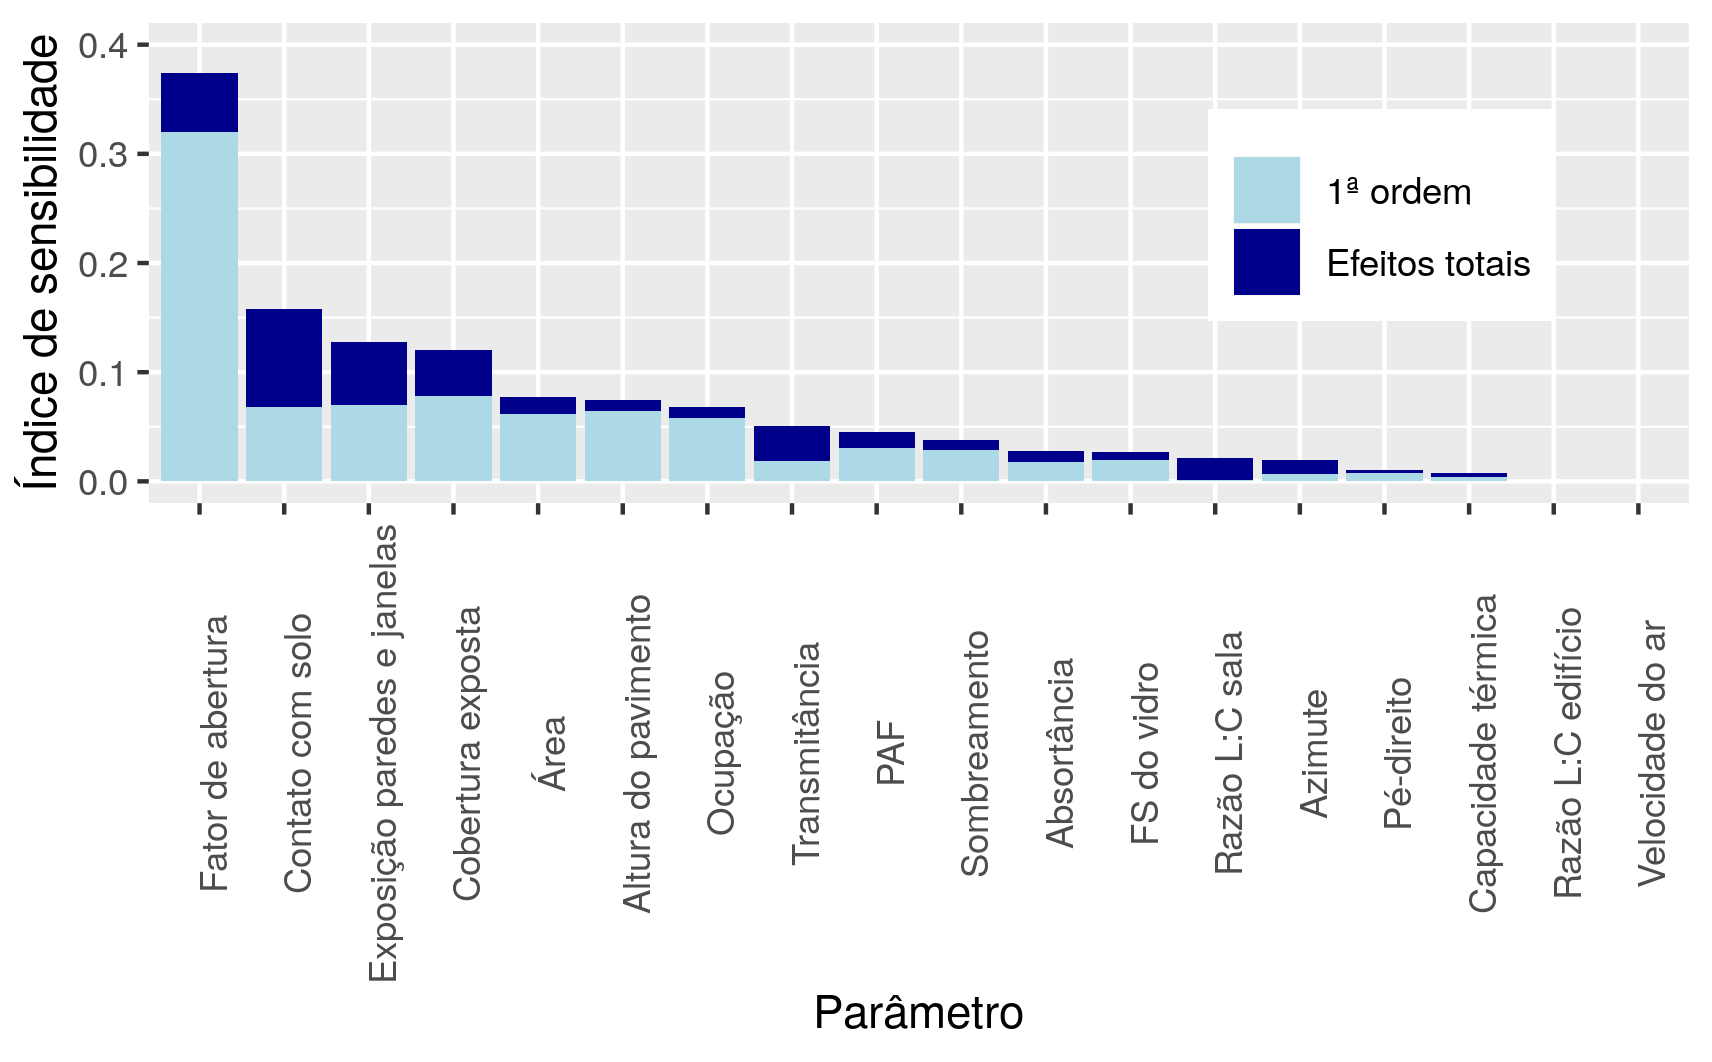
\includegraphics[width=1\linewidth]{img/as_temp.png}
	\label{fig:as_temp}
	%			\begin{flushleft}
	%				Fonte: o autor.
	%			\end{flushleft}
\end{figure}

\begin{figure}[H]
	\centering
	\caption{AS de Sobol dos efeitos de primeira ordem e efeitos totais no EHF}
	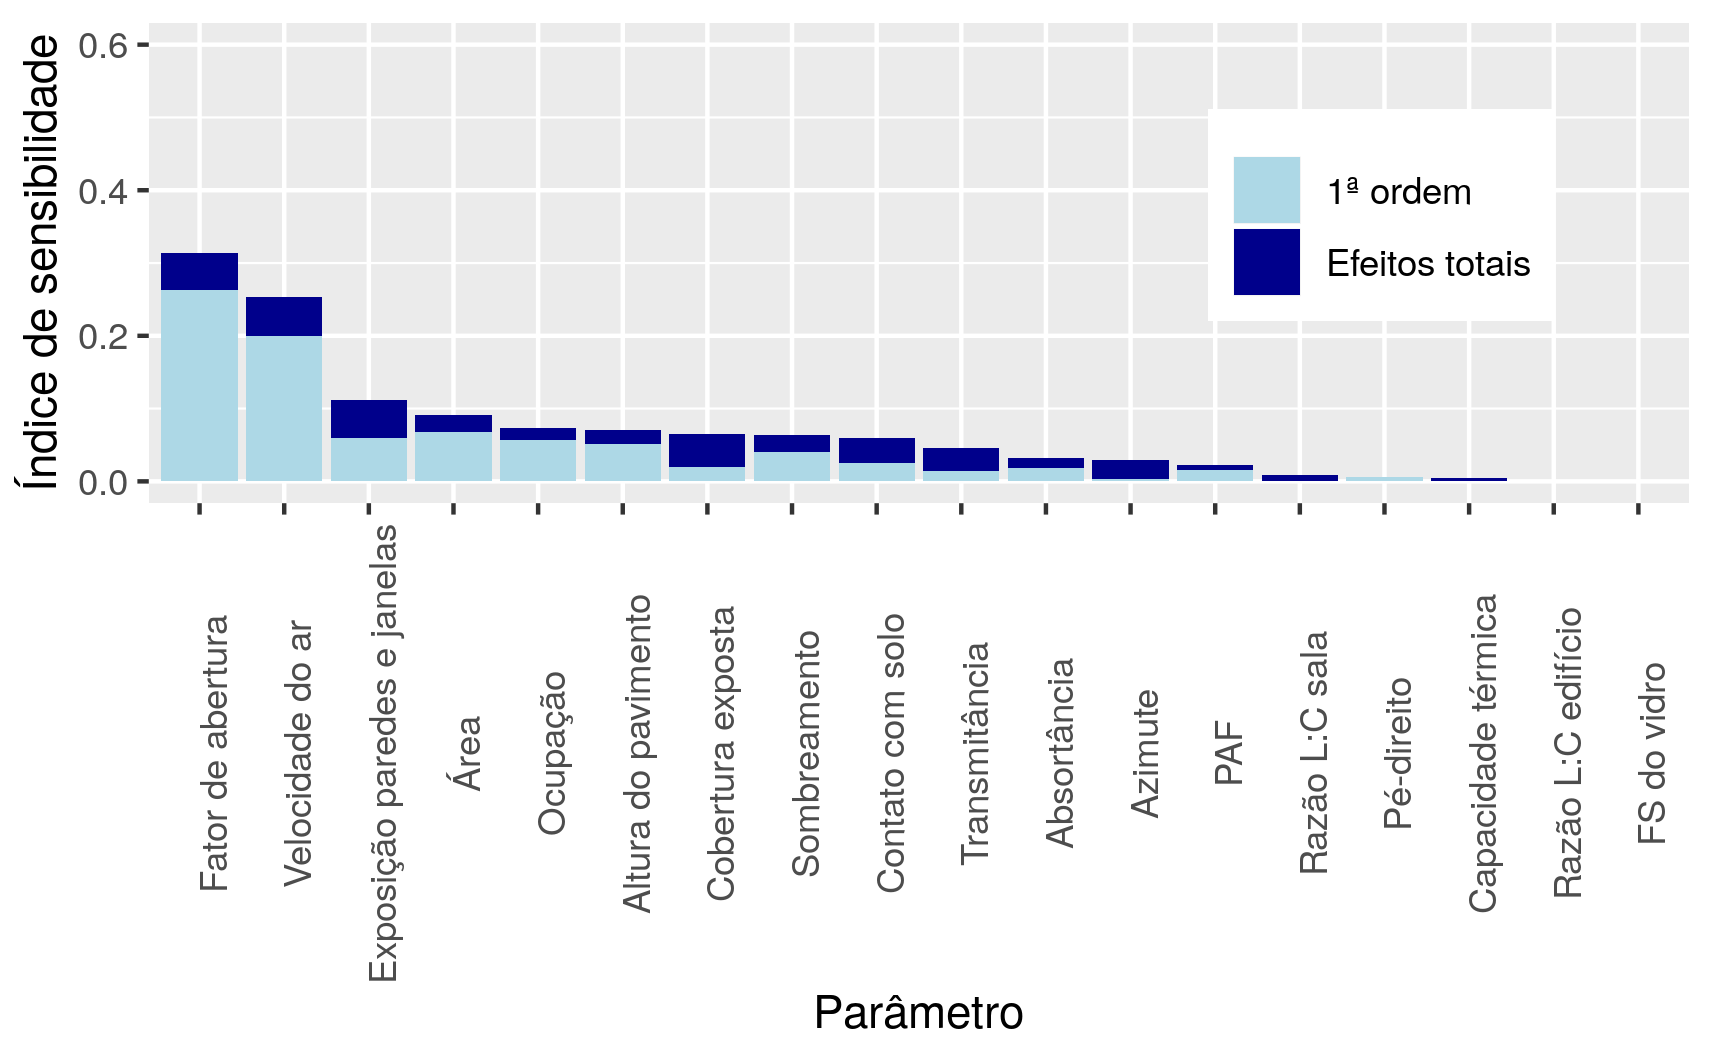
\includegraphics[width=1\linewidth]{img/as_ehf.png}
	\label{fig:as_ehf}
	%			\begin{flushleft}
	%				Fonte: o autor.
	%			\end{flushleft}
\end{figure}

Os parâmetros mais influentes nas ACH, como esperado, são aqueles relacionados às aberturas da zona. 
O primeiro parâmetro de maior influência é o fator de abertura das janelas, seguido do parâmetro relacionado à exposição das paredes e à presença de VN cruzada ou unilateral. A área tem influência significativa, pois o cálculo das trocas de ar leva em conta o volume de ar na zona, que é diretamente relacionado à sua área. 
A altura do pavimento é determinante nos resultados do ACH, pois a velocidade do vento no EnergyPlus é calculada em função da altura da zona.
A orientação da zona (azimute) não tem uma influência significativa de primeira ordem. No entanto, percebe-se uma influência mais significativa considerando-se os efeitos totais. 
O azimute é determinante para a definição dos coeficientes de pressão sobre as fachadas da edificação. Por isso, a influência deste parâmetro nos resultados das simulações depende de outros parâmetros, relacionados ao posicionamento e às áreas das aberturas na zona.
A velocidade do ar não influencia os resultados relacionados ao ACH, pois é considerada apenas após o término das simulações, ao se calcular o EHF.
A AS apresentou interações de segunda ordem significativas entre o fator de abertura das janelas e a presença de VN cruzada ou unilateral, com um índice de sensibilidade igual a 0,121.
Contudo, o parâmetro com maiores interações de segunda ordem relacionados ao ACH foi o PAF, com a soma dos índices de segunda ordem igual a 0,300.

As análises relacionadas à temperatura operativa e ao EHF indicam relevância dos parâmetros relacionados à VN. Para ambas as análises, o parâmetro mais influente foi o fator de abertura da janela, enquanto o parâmetro relacionado à exposição das paredes e à presença de VN cruzada ou unilateral foi o terceiro mais influente. 
O contato com o solo apresentou-se como o segundo parâmetro mais influente nas médias anuais de temperatura operativa, considerando-se os esfeitos totais. No entanto, a influência deste parâmetro não é tão significativa no EHF. Isso indica que a influência do contato com o solo nas temperaturas operativas das zonas é mais significativa em faixas de temperatura que não interferem no cálculo do EHF, ou seja, consideravelmente a cima ou abaixo dos limites superiores de aceitabilidade estabelecidos pelo método de conforto adaptativo.
Observa-se que os efeitos totais entre o segundo (contato com o solo) e o quarto (exposição da cobertura) índice de sensibilidade com valores mais altos na AS relacionada à média anual da temperatura operativa são expressivos.
A transmitância das paredes, o azimute, e a razão entre a largura e o comprimento da sala também apresentam efeitos totais relevantes, apesar dos baixos índices de sensibilidade para primeira ordem. Isso indica que há interações significativas entre esses parâmetros e os demais.

O movimento do ar apresenta-se como o segundo parâmetro mais influente nos resultados de EHF, o que indica um grande potencial de uso de ventiladores na busca por conforto térmico nos ambientes. 
A área da zona e a densidade de ocupação apresentaram-se mais influentes nos resultados de EHF, comparando-se aos resultados relacionados às médias anuais de temperatura operativa.
O azimute, apesar de seu índice de sensibilidade baixo para a análise de primeira ordem, apresentou índices de segunda ordem expressivos. As interações de segunda ordem ocorrem relacionadas a parâmetros referentes à VN e a parâmetros referentes à radiação solar. A soma dos índices de segunda ordem do azimute em relação ao EHF foi igual a 0,177.  %, como sombreamento e absortância

A complexidade dos fenômenos representados junto às interações entre as diferentes variáveis exige um grande número de casos para reduzir incertezas, pois o método de AS utiliza uma base amostral. Por isso, existe uma incerteza associada aos índices de sensibilidade obtidos nas AS conduzidas, e a soma dos valores dos índices ultrapassa o valor 1. Entretanto, a aplicação da análise de sensibilidade global ofereceu resultados relevantes para o trabalho, com índices de sensibilidade condizentes aos comportamentos físicos representados pelas simulações. 

Baseando-se nos resultados das AS, alguns dos parâmetros não foram considerados para o desenvolvimento do metamodelo. A Tabela \ref{table:param_fixed} apresentam os parâmetros que tiveram seus valores fixos. O valor do pé-direito foi determinado considerando-se o valor encontrado com mais frequência na base de dados analisada. A capacidade térmica da parede foi estabelecida de acordo com o valor de uma parede de bloco cerâmico de dimensões 14x19x29 cm, e argamassa de 2,5 cm. Os parâmetros relacionados às proporções entre largura e profundidade das salas e edifícios foram determinados com valor igual a 1. 

\begin{table}[H]		
	\centering
	\caption{Parâmetros com valores constantes.}
	\label{table:param_fixed}
	\begin{tabular}{|l |c |}
		\hline
		\textbf{Parâmetro} & Valor fixo \\
		\hline
		Razão L:C do edifício (-) & 1 \\
		\hline
		Razão L:C da sala (-) & 1 \\
		\hline
		Pé-direito (m) & 2,5 \\
		\hline
		Capacidade térmica (kJ/m$^2$K) & 161 \\
		\hline
		%			Fator solar do vidro (-) & 0,87 \\
		%			\hline
	\end{tabular}
\end{table}

%	Occupant density is the most influential parameter
%	on EHF, since it obtained the highest index value for
%	first order, second order and total effects. From the
%	first order effects indices, it was observed that, after
%	occupant density, the contact with the ground and
%	the window opening factor are the most influential
%	parameters on both EHF and average Operative Tem-
%	perature. The index values for these two outputs are
%	similar overall, since EHF is calculated from the Op-
%	erative Temperature. Therefore, the annual average
%	Operative Temperature results were not plotted. The
%	most influential parameters on the ACH are, as ex-
%	pected, the ones related to the zone’s openings. They
%	are: opening factor of the window; exposure condition
%	of walls and windows; and WWR.
%	Significant colinearities are identified among the pa-
%	rameters. Even though the zone area has a higher
%	first order index, the exposure of the walls and the
%	roof could be more influential on the EHF, when com-
%	bined with certain parameters. Second order effects
%	analysis shows high interaction between the exterior
%	walls exposure and the opening factor of the win-
%	dow. The interaction could be explained due to the
%	the higher influence of either one or two windows on
%	the facade when the window opening factor is higher.
%	The highest second order effect index for EHF was
%	the one relating occupant density and ground expo-
%	sure. These two parameters were also the two most
%	influential for first order and total effects analyses.
%	
%	Thus, this strong relation points out how contact with
%	the ground can help to dissipate internal heat gains
%	at the climate of Sao Paulo.
%	Based on the SA results, some the least influential
%	parameters were not considered as input features for
%	the final model. They are: height of the zone’s floor;
%	SHGC; wall thermal capacity; shading device; build-
%	ing ratio.

\subsection{Desenvolvimento do metamodelo}

A partir das 20.000 simulações geradas para o treinamento da rede neural artificial (RNA). %, obteve-se resultados de EHF variando entre 0,00 e 1,00.
O metamodelo final foi definido com 14 parâmetros:
\begin{itemize}
	\item Fator de abertura das janelas;
	\item Velocidade do ar;
	\item Condição de exposição das paredes e janelas;
	\item Área da sala;
	\item Densidade de ocupação;
	\item Altura do pavimento;
	\item Exposição da cobertura;
	\item Sombreamento horizontal;
	\item Contato com o solo;
	\item Transmitância das paredes;
	\item Absortância das paredes;
	\item Fator solar do vidro;
	\item Azimute da sala;
	\item PAF.
\end{itemize}

Os parâmetros variaram na mesma faixa de valores estabelecida na primeira etapa deste estudo. O ângulo do azimute da sala é determinado considerando-se o eixo entre a parede voltada para a circulação e a parede oposta.

O contato com o solo e a exposição da cobertura foram definidas como variáveis binárias, com o valor zero correspondendo à superfície adiabática, e 1 correspondendo à exposição.
O parâmetro que representa a condição de exposição das paredes e janelas não foi representado com valores numéricos, e sim como uma variável de fatores, com cinco opções de exposição. Além das três opções apresentadas na Figura \ref{fig:exp_sz}, considerou-se as exposições espelhadas. 	
Os demais parâmetros foram normalizados com valores entre -1 e 1.

\begin{figure}[H]
	\centering
	\caption{Condição de exposição das paredes e janelas.}
	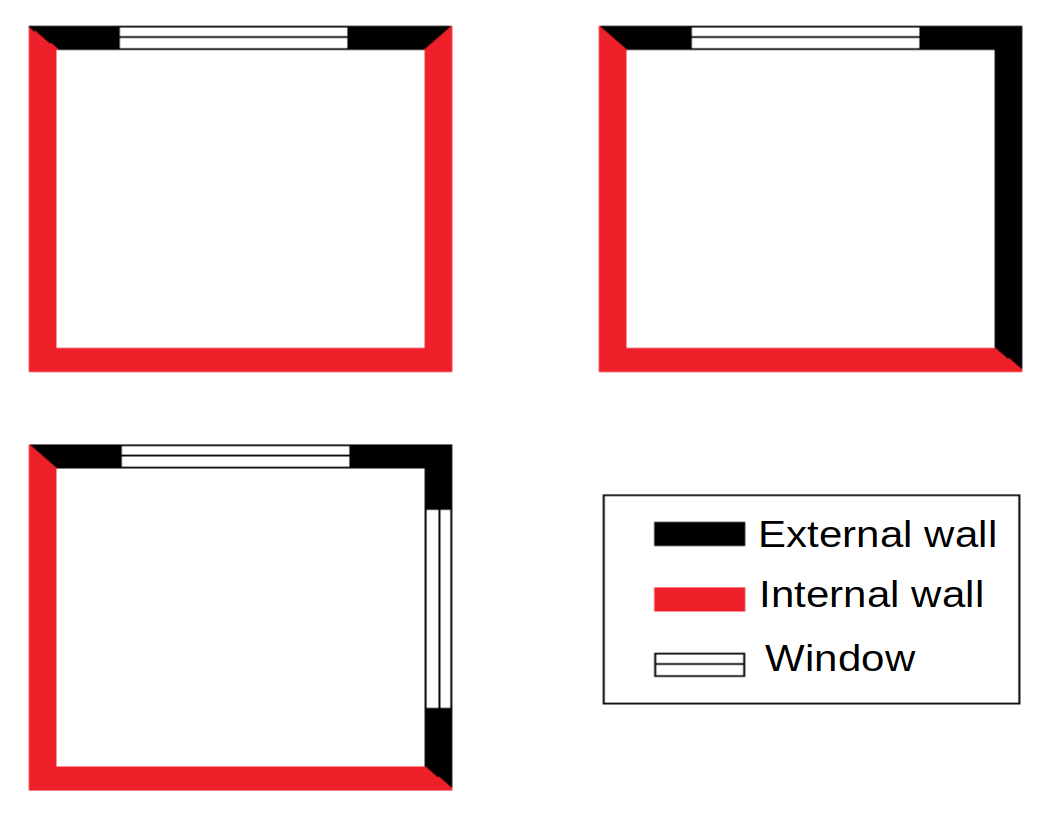
\includegraphics[width=1\linewidth]{img/wallexposition.png}
	\label{fig:exp_sz}
	%			\begin{flushleft}
	%				Fonte: o autor.
	%			\end{flushleft}
\end{figure}

O modelo de RNA final foi definido com duas camadas, umas de 50 nós, e a outra com 20. 
O algorítimo de otimização que obteve o melhor desempenho foi o \textit{Adagrad's Optimizer}, disponibilizado pela biblioteca \textit{TensorFlow}, com uma taxa de aprendizagem igual a 0,05.

A Figura \ref{fig:ann_validation} apresenta um gráfico de pontos comparando os resultados de EHF obtidos para as simulações e para as estimativas da RNA, a partir da base de dados desenvolvida para a validação do metamodelo. A base de dados para a validação teve apenas os parâmetros incluídos no treinamento da RNA variados. 
O erro absoluto médio do EHF para os casos de validação foi 0,0104, com o AE95 igual a 0,0226.

\begin{figure}[H]
	\centering
	\caption{Condição de exposição das paredes e janelas.}
	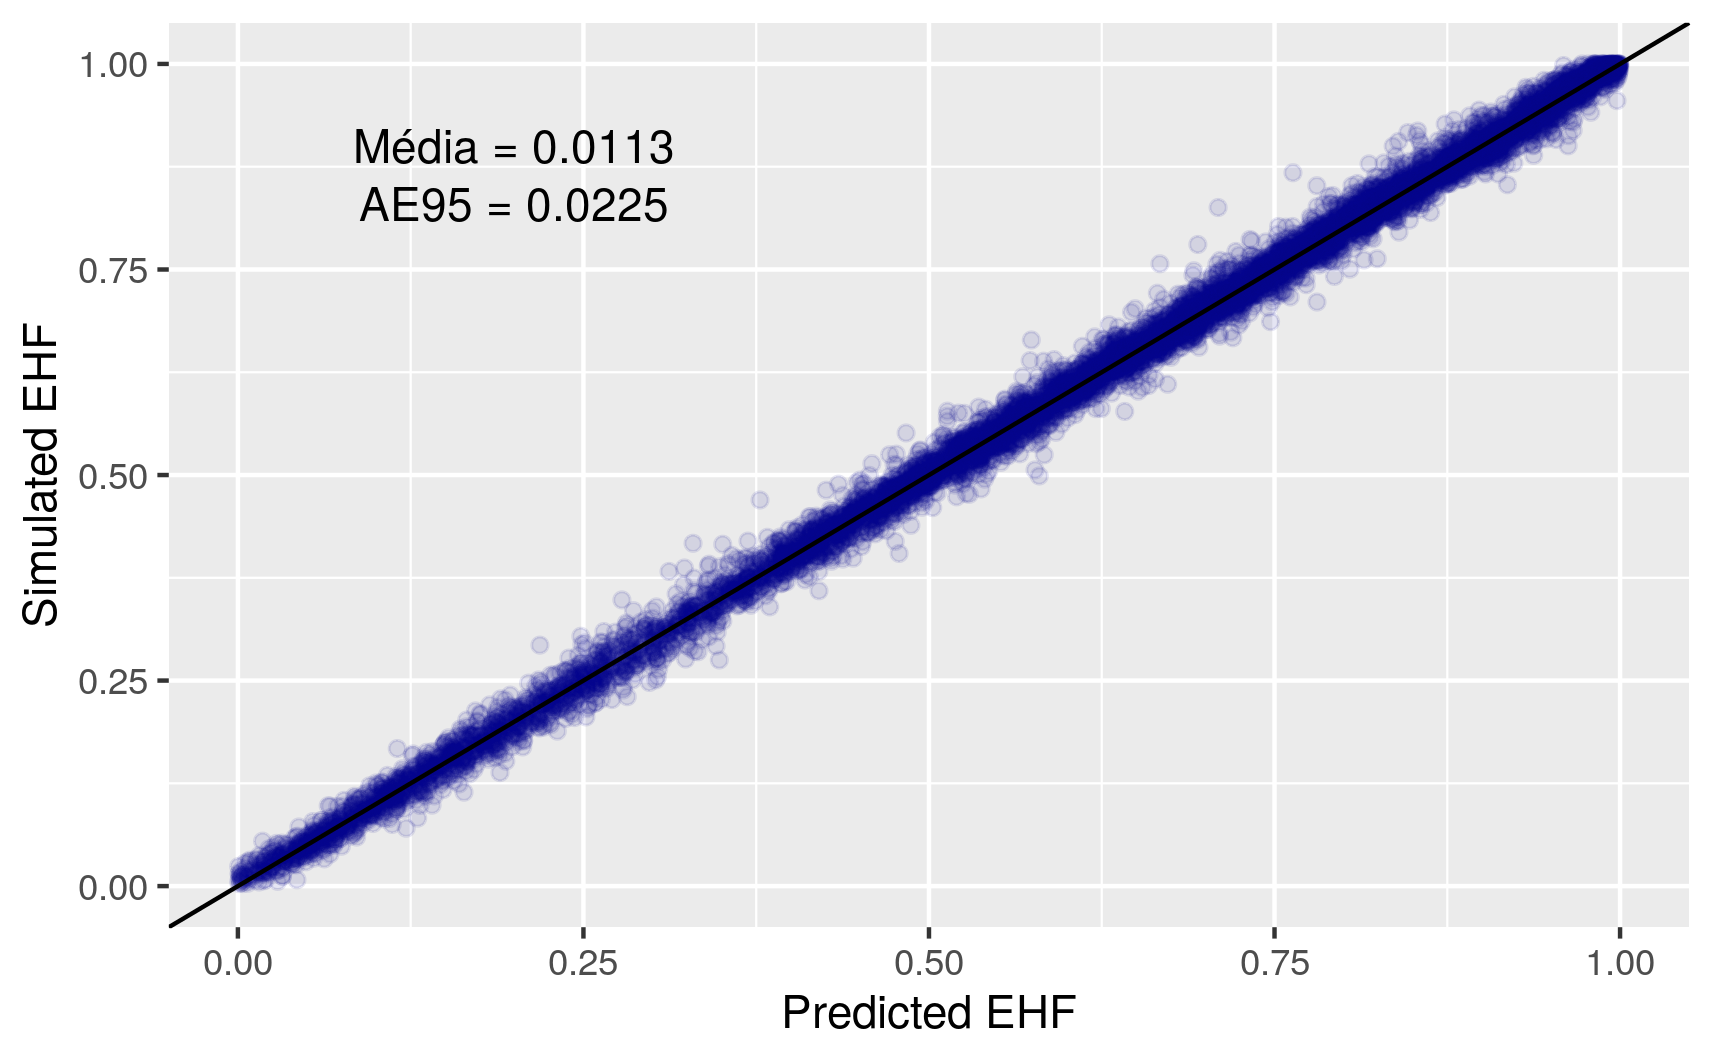
\includegraphics[width=1\linewidth]{img/ann_validation.png}
	\label{fig:ann_validation}
\end{figure}

Outra comparação foi conduzida com a amostragem utilizada para a AS. Essa base de dados estava disponível, e não foi utilizada pra o desenvolvimento da RNA, então ela foi escolhida para testar o desempenho da RNA quando todos os parâmetros avaliados neste estudo variam. A Figura \ref{fig:ann_sobol} apresenta o gráfico de pontos comparando os resultados de EHF obtidos para as simulações e para as estimativas da RNA, a partir da base de dados da AS de sobol. O erro absoluto médio do EHF para os casos de validação foi 0,0104, com o AE95 igual a 0,0226.

\begin{figure}[H]
	\centering
	\caption{Condição de exposição das paredes e janelas.}
	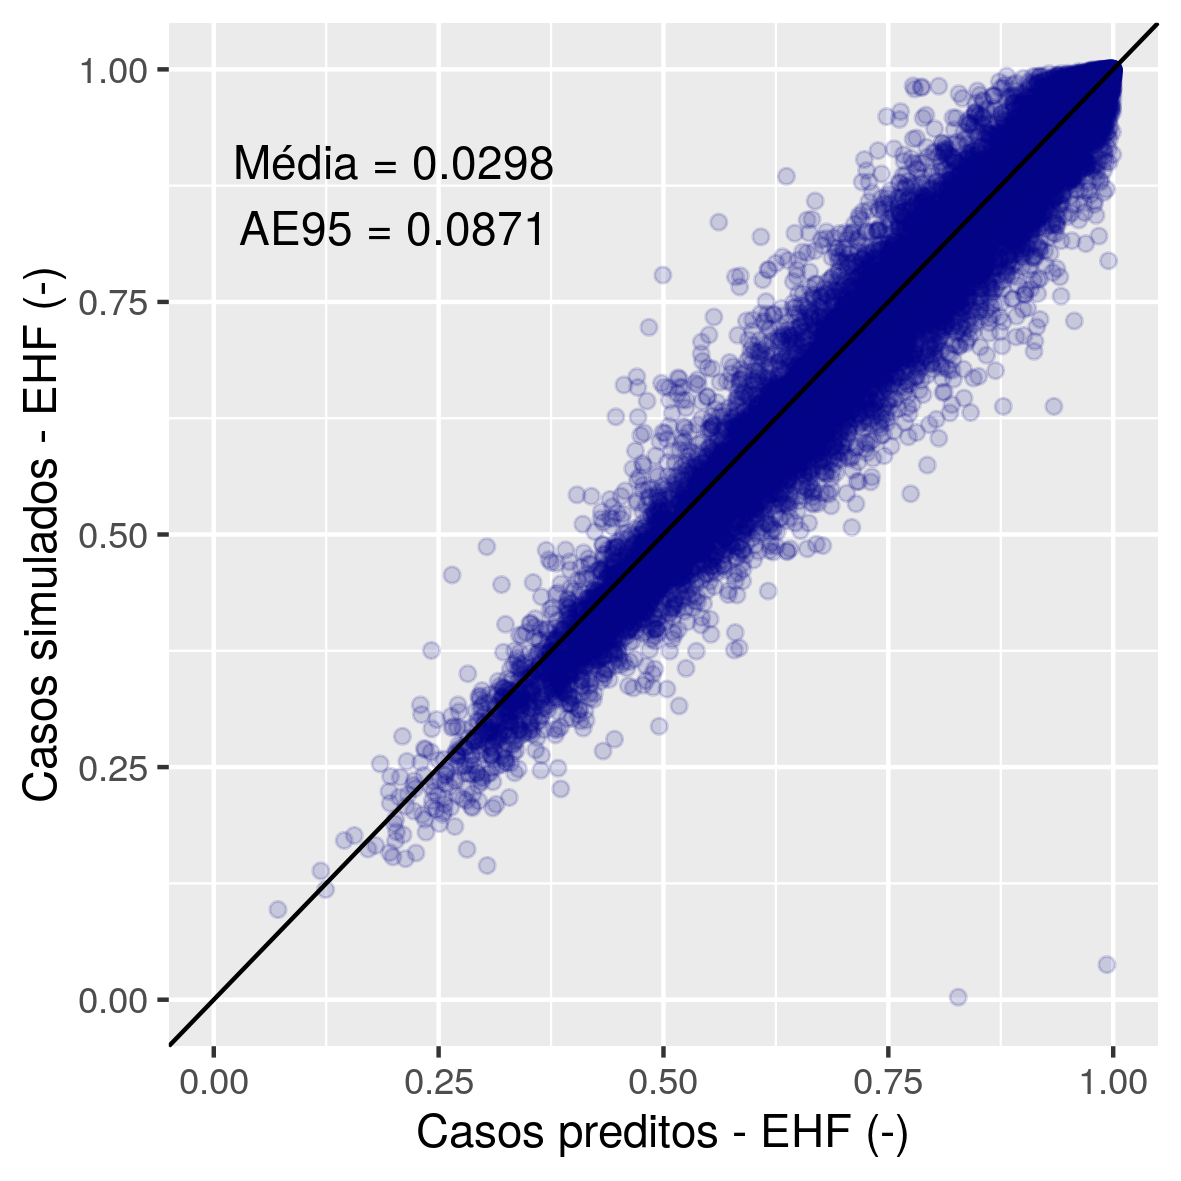
\includegraphics[width=1\linewidth]{img/ann_test.png}
	\label{fig:ann_sobol}
\end{figure}

\chapter{Conclusões}
\label{chapter:conclusoes}
	

\section{Limitações e justificativas}

%As limitações desse estudo são indicadas em conformidade com a ordem de execução das etapas de desenvolvimento:
%
%\begin{itemize}
%	\item Lorem ipsum dolor sit amet, consectetur adipiscing elit. Nulla commodo, augue non consectetur vehicula, felis velit commodo eros, nec bibendum augue purus quis mi. Donec dapibus id magna eget euismod;
%	
%	\item Lorem ipsum dolor sit amet, consectetur adipiscing elit. Nulla commodo, augue non consectetur vehicula, felis velit commodo eros, nec bibendum augue purus quis mi. Donec dapibus id magna eget euismod;
%	
%	\item Lorem ipsum dolor sit amet, consectetur adipiscing elit. Nulla commodo, augue non consectetur vehicula, felis velit commodo eros, nec bibendum augue purus quis mi. Donec dapibus id magna eget euismod.
%	
%\end{itemize}

\section{Sugestões para trabalhos futuros}

%As sugestões para trabalhos futuros são indicadas em conformidade com as potencialidades expressas nesse estudo, sendo:
%
%\begin{itemize}
%	\item Lorem ipsum dolor sit amet, consectetur adipiscing elit. Nulla commodo, augue non consectetur vehicula, felis velit commodo eros, nec bibendum augue purus quis mi. Donec dapibus id magna eget euismod;
%
%	\item Lorem ipsum dolor sit amet, consectetur adipiscing elit. Nulla commodo, augue non consectetur vehicula, felis velit commodo eros, nec bibendum augue purus quis mi. Donec dapibus id magna eget euismod;
%
%	\item Lorem ipsum dolor sit amet, consectetur adipiscing elit. Nulla commodo, augue non consectetur vehicula, felis velit commodo eros, nec bibendum augue purus quis mi. Donec dapibus id magna eget euismod.
%	
%\end{itemize}

%\begin{appendices}
%	\chapter{Classificação climática de Köppen-Geiger}
%	\begin{figure}[!h]
%		\centering
%		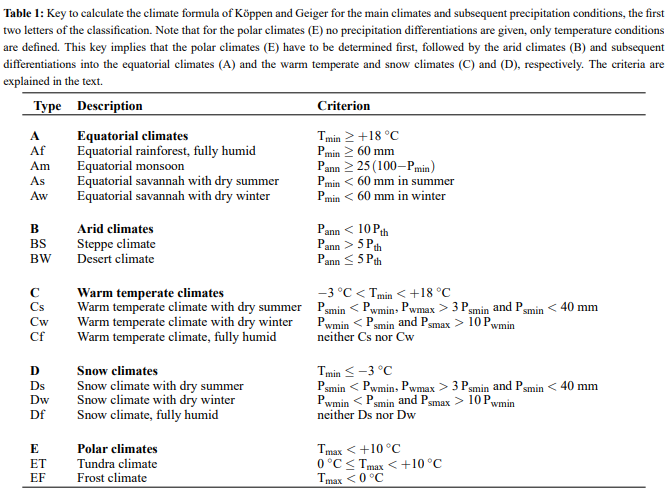
\includegraphics[width=1\linewidth]{img/tablekoppengeiger1.png}
%		\label{fig:tablekoppengeiger1}
%	\end{figure}
%\end{appendices}
%
%\begin{appendices}
%	\chapter{Código...}
%	\lstset{language=c++}
%	\lstset{label={lst:code_direct}}
%	\lstset{basicstyle=\tiny}	
%	\lstinputlisting{code/code.cc}
%\end{appendices}

%\bibliographystyle{lib/abntex2-num}
%\bibliographystyle{lib/abntex2-alf}
%\bibliography{citacoes}
\bibliography{library}
	
\end{document}